\documentclass{article}
\usepackage{graphicx}
\usepackage{amsmath}
\usepackage{amssymb}
\usepackage{listings}
\usepackage{xcolor}
\usepackage{tocloft}
\usepackage[utf8]{inputenc}
\usepackage[T1]{fontenc}
\usepackage{tgbonum}
\usepackage{titlesec}
\usepackage{fancyhdr}
\usepackage{lipsum}
\usepackage{hyperref}

\titleformat{\section}[hang]{\normalfont\Large\bfseries}{\thesection}{1em}{}[\titlerule]
\newcommand{\authorname}{Alper Karaca}

\fancyhf{}
\fancyhead[R]{\authorname}
\renewcommand{\headrulewidth}{0pt}

\fancyfoot[R]{\thepage}

\pagestyle{fancy}

\cftsetindents{section}{0em}{3em}
\cftsetindents{subsection}{0em}{4em}

\renewcommand\cfttoctitlefont{\hfill\Large\bfseries}
\renewcommand\cftaftertoctitle{\hfill\mbox{}}

\setcounter{tocdepth}{2}

\title{Veri Yapilari Notlar (www.cyberdatascience.com.tr)}
\author{Alper Karaca}
\date{January 2024}

\definecolor{dkgreen}{rgb}{0,0.6,0}
\definecolor{gray}{rgb}{0.5,0.5,0.5}
\definecolor{mauve}{rgb}{0.58,0,0.82}

\lstset{frame=tb,
	language=Python,
	aboveskip=3mm,
	belowskip=3mm,
	showstringspaces=false,
	columns=flexible,
	basicstyle={\small\ttfamily},
	numbers=none,
	numberstyle=\tiny\color{gray},
	keywordstyle=\color{blue},
	commentstyle=\color{dkgreen},
	stringstyle=\color{mauve},
	breaklines=true,
	breakatwhitespace=true,
	tabsize=3
}

\begin{document}

\maketitle

\newpage
\tableofcontents
\newpage

\section{Big-O Notation}

Big-O Notation, algoritmaların verimliliğini ve performansını değerlendirmek için kullanılan matematiksel bir gösterimdir. Bir algoritmanın giriş boyutu (b) büyüdükçe nasıl davrandığını gösterir. Bu gösterim, algoritmanın en kötü senaryoda nasıl bir performans sergileyeceğini anlatır. Asıl odak, algoritmanın performansının giriş boyutu büyüdükçe ne kadar arttığıdır. Big-O değeri, algoritmanın giirş boyutuna göre ne kadar hızlı arttığını belirler. Hesaplama yapılırken şu faktörler dikkate alınır:

\begin{itemize}
    \item \textbf{Döngüler (Loops)}: Her döngü, giriş boyutuna bağımlı olarak çalışır.
    \item \textbf{Yinelemeli (Recursive) Fonksiyonlar}: Fonksiyonlar kendilerini çağırdıklarında, üstel veya logaritmik bir büyüme sergilerler.
    \item \textbf{Operasyonlar (Operations)}: Veri yapılarında yapılan listeleme, ekleme, silme gibi işlemler, yapının tipine göre farklı Big-O değerine sahiptir.
\end{itemize}

\subsection{Space Complexity (Bellek Karmaşıklığı)}

Space Complexity, algoritma çalışırken kullandığı ekstra bellek miktarını temsil eder. Bir algoritmanın çalışırken ihtiyaç duyduğu toplam bellek miktarını ifade eder. Space Complexity, sadece programın çalışması için gereken ekstra bellek miktarını ölçer. Girdinin zaten kendisinin kapladığı bellek dikkate alınmaz. Amacı, bir algoritmanın ne kadar verimli bir şekilde bellek kullandığını belirlemektir.

\subsection{Time Complexity (Zaman Karmaşıklığı)}

Time Complexity, bir algoritmanın çalışması için gereken süreyi, girdi boyutu (n) büyüdükçe ifade eder. Algoritmanın gerçekleştirdiği işlem sayısını ve bu işlemlerin zaman maliyetlerini analiz eder. Girdi boyutu büyüdükçe, algoritmanın ne kadar hızlı çalışacağını tahmin eder. Amacı, bir algoritmanın zaman verimliliğini ölçmek ve büyük veri setleriyle nasıl ölçeklendiğini anlamaktır.

\subsection{Big-O Notation Türleri}

\begin{enumerate}
    \item \textbf{O(1) - Sabit Zaman}:
    \begin{itemize}
        \item Algoritma, giriş boyutundan bağımsız olarak her zamana aynı sürede çalışır.
        \item Örneğin; dizideki bir elemana doğrudan erişim (indexleme).
    \end{itemize}
    \item \textbf{O(logn) - Logaritmik Zaman}:
    \begin{itemize}
        \item Giriş boyutu arttıkça çalışma zamanı logaritmik olarak artar.
        \item Örneğin; ikili arama algoritması.
    \end{itemize}
    \item \textbf{O(n) - Doğrusal Zaman}:
    \begin{itemize}
        \item Giriş boyutuyla doğrusal olarak artar. Girdi ne kadar büyükse, algoritma o kadar uzun sürede çalışır.
        \item Örneğin; bir listeyi döngüyle baştan sona taramak.
    \end{itemize}
    \item \textbf{O(nlogn) - Doğrusal Logaritmik Zaman}:
    \begin{itemize}
        \item Verimli sıralama algoritmalarında görülür.
        \item Örneğin; hızlı sıralama (quick sort), birleştirme sıralaması (merge sort).
    \end{itemize}
    \item \textbf{O($n^2$) - Karesel Zaman}:
    \begin{itemize}
        \item Giriş boyutu büyüdükçe çalışma zamanı karesel olarak artar.
        \item Örneğin; çift döngüyle çalışan sıralama algoritmaları (bubble sort).
    \end{itemize}
    \item \textbf{O($2^n$) - Üstel Zaman}:
    \begin{itemize}
        \item Giriş boyutu arttıkça çalışma süresi üstel olarak artar.
        \item Örneğin; bazı yinelemeli çözümler (fibonacci serisi).
    \end{itemize}
    \item \textbf{O(n!) - Faktöriyel Zaman}:
    \begin{itemize}
        \item Çok büyük veri kümeleri için inanılmaz derecede yavaş çalışan algoritmalar.
        \item Örneğin; tüm olası permütasyonları hesaplamak.
    \end{itemize}
\end{enumerate}

\subsection{Sadeleştirme - Drop Constants (Sabitleri Atma)}

Sabitleri atma yöntemi, Big-O notasyonunda yer alan sabit katsayıların büyümeyi etkilemediğini varsayarak, bunları Big-O ifadesinden çıkarma işlemidir. Sabit bir katsayı, büyüme oranını etkilemediği için sadeleştirilir. Giriş boyutu (n) büyüdükçe sabit faktörlerin etkisi giderek küçülür ve böylece ihmal edilebilir hale gelir. Örneğin;

\begin{lstlisting}[language=Python]
def print_elements_twice(arr):
    for i in arr:
        print(i)

    for i in arr:
        print(i)
\end{lstlisting}

Bu fonksiyon, girdi içerisindeki her bir elemanı iki kere yazdırır. İki ayrı döngü ile elemanları iki kez dolaştığı için çalışma süresi;

\begin{itemize}
    \item \textbf{Birinci döngü}: $O(n)$
    \item \textbf{İkinci döngü}: $O(n)$
    \item \textbf{Toplam}: $O(n) + O(n) = O(2n)$
\end{itemize}

Çalışma süresi $O(2n)$'dir fakat Big-O sadeleştirilerek $O(n)$ olarak yazılır çünkü "2" ihmal edilir.

Bir başka örnekte ise;

\begin{lstlisting}[language=Python]
def example_func(arr):
    for i in arr:
        for j in arr:
            print(i, j)

    print("Done")
\end{lstlisting}

Bu fonksiyon iki döngü çalıştırır ve her bir elemanı diğeriyle birlikte yazdırır:

\begin{itemize}
    \item İç içe iki döngü: $O(n^2)$
    \item Sabit bir çıktı: $O(1)$
\end{itemize}

Toplamda bu algoritmanın karmaşıklığı $O(n^2 + 1)$ olur. Ancak sabit terim $O(1)$, giriş boyutu büyüdükçe önemini kaybedeceği için ihmal edilir. Böylece sonuç $O(n^2)$ olur.

\subsection{Sadeleştirme - Drop Non-Dominant Terms (Baskın Olmayan Terimleri Atma)}

Büyük giriş boyutlarında baskın olmayan, daha küçük büyüme hızına sahip terimler ihmal edilir. En büyük büyüme hızına sahip olan terim, giriş boyutu arttıkça algoritmanın performansını en çok etkileyen terimdir. Bu yüzden baskın olmayan terimleri atarak sadeleştirme yapılır.

\begin{lstlisting}[language=Python]
def example_func(arr):
    for i in arr:
        for j in arr:
            print(i, j)
    for i in arr:
        print(i)
\end{lstlisting}

Bu fonksiyon iki bölümden oluşur:

\begin{itemize}
    \item İç içe iki döngü: $O(n^2)$
    \item Tek bir döngü: $O(n)$
\end{itemize}

Toplamda algoritmanın karmaşıklığı $O(n^2 + n)$ olur. Ancak giriş boyutu büyüdükçe $O(n^2)$ terimi baskın hale gelir, çünkü $n^2$, $n$'den daha hızlı büyür. Bu yüzden $O(n^2 + n)$ ifadesinden baskın olmayan $O(n)$ terimi atılır ve sonuç $O(n^2)$ olur.

\newpage
\section{Theta Notation}

Bir algoritmanın çalışma süresinin veya bellek kullanımının en iyi ve en kötü durumlarını birleştirerek bir üst ve alt sınır sağlar. Theta notasyonu, bir algoritmanın belirli bir giriş boyutu için zaman veya alan karmaşıklığını kesin bir şekilde belirtir. Bir algoritmanın asimptotik davranışını daha iyi anlamak için, karmaşıklık analizi yaparken diğer notasyonlarla (Omage notasyonu, O notasyonu) birlikte kullanır.

\[ c_1 \cdot f(n) \leq T(n) \leq c_2 \cdot f(n) \]

Burada:

\begin{itemize}
    \item $c_1$ ve $c_2$: Pozitif sabitlerdir.
    \item $n$: Giriş boyutunu temsil eder.
    \item $T(n)$: Algoritmanın karmaşıklığıdır.
    \item $f(n)$: Algoritmanın karmaşıklığını temsil eden fonksiyondur.
\end{itemize}

\begin{lstlisting}[language=Python]
def bubble_sort(arr):
    n = len(arr)
    for i in range(n):
        for j in range(0, n - i  -1):
            if arr[j] > arr[j + 1]:
                arr[j], arr[j + 1] = arr[j + 1], arr[j]
    return arr
\end{lstlisting}

Bu kod, Bubble Sort algoritmasını temsil eder. Algoritma, dzinin her elemanını karşılaştırarak sıralar. İçteki döngü, dıştaki döngü ile çarpılarak toplamda $\frac{n(n-1)}{2}$ karşılaştırma yapar. Bu, $\frac{n^2}{2} - \frac{n}{2}$ kadar karşılaştırma eder. İç içe iki for olduğu için Big-O notasyonu $O(n^2)$'dir. Dış döngü için toplam $n$ adet iterasyon yapılır. İç döngü içn toplam $\frac{n(n-1)}{2}$ adet iterasyon yapılır. Bu nedenle toplam karmaşıklık:

\[ T(n) = O(n^2) \]

Bubble algoritması hem en iyi durumda hem de en kötü durumda benzer bir performans sergiler;

\begin{itemize}
    \item \textbf{En İyi Durum}: Dizi zaten sıralıysa, yine tüm karşılaştırmalar yapılır, $\Theta(n^2)$.
    \item \textbf{En Kötü Durum}: Dizi tamamen ters sıralıysa, yine tüm karşılaştırmalar yapılır, $\Theta(n^2)$.
\end{itemize}

\newpage
\section{Omega Notation}

Omega notasyonu, algoritmaların zaman karmaşıklığını ifade etmek için kullanılan bir notasyondur. En iyi durum analizini yapmak için kullanılır ve algoritmanın en az ne kadar süre alacağını belirtir. Bu, algoritmanın çalışma süresinin alt sırasını tanımlar.

\[ T(n) = \Omega(f(n)) \]

Burada:

\begin{itemize}
    \item $T(n)$: Algoritmanın çalışma süresi (giriş boyutu n için).
    \item $f(n)$: Algoritmanın en iyi durum karmaşıklığını temsil eden fonksiyon.
\end{itemize}

Bir algoritmanın $\Omega$ notasyonu ile tanımlanabilmesi için, aşağıdaki koşulların sağlanması gerekir:

\begin{enumerate}
    \item Pozitif bir $c$ sayısı ve $n_0$ sayısı bulunmalıdır.
    \item Tüm $n \geq n_0$ için $T(n) \geq c \cdot f(n)$ olmalıdır.
\end{enumerate}

Örneğin bir algoritmanın çalışma süresi $T(n) = 3n^2 + 2n + 1$ olsun. Bu durumda, $T(n)$ için $\Omega$ notasyonunu hesaplamak istersek:

\begin{enumerate}
    \item En baskın terimi belirleriz.
    \item Bu durumda $f(n) = n^2$ olacaktır.
    \item $T(n) = \Omega(n^2)$ olarak ifade edilebilir.
\end{enumerate}

Sonuç olarak, bu algoritmanın en iyi durumu en az $c \cdot n^2$ kadar süre alır.

\newpage
\section{Array (Dizi)}

Array, belirli bir veri tipinde sabit boyutta, ardışık bellek konumlarında depolanan öğelerin koleksiyonudur. Array, aynı türden verileri saklamak için kullanılır. Array oluşturulurken boyutu belirlenir ve bu boyut programın çalışma süresi boyunca değişmez. Array, homojen veri tipine sahiptir yani array içerisindeki tüm elemanlar aynı veri tipine sahip olmalıdır. Array'in elemanlarına index numarası kullanılarak doğrudan erişilebilir. Bu $O(1)$ zaman karmaşıklığı ile gerçekleştirilir. Array elemanları bellekte ardışık olarak saklanır, bu da bellekteki bellek adresleri arasında kesintisiz bir yapı sağlar. Bu, bellek yönetimi açısından avantajlıdır.

Array, bellekte ardışık bellek alanları üzerinde depolandığı için bellekte başlangıç adresi ve bu adres üzerinden yapılan indeksleme ile erişim sağlanır. Bellekte bir array oluşturulduğunda, belleğin bir kısmı ayrılır ve elemanlar bu alana yerleştirilir.

Array'ler iki tiptedir:

\begin{itemize}
    \item \textbf{Tek Boyutlu Array (One-Dimensional Array)}: Elemanların tek bir sıra halinde sıralandığı array türüdür. Elemanlara yalnızca bir index ile erişilir. Bellekte ardışık olarak saklanır.
    \item \textbf{Çok Boyutlu Array (Multi-Dimensional Array)}: Birden fazla boyutta elemanlar içeren array türüdür. Elemanlara birden fazla index kullanılarak erişilir. Bellekte ardışık olarak saklanır.
\end{itemize}

\subsection{Erişim (Access)}

Array'deki bir elemana erişmek, elemanın index numarasını kullanarak doğrudan yapılır. Erişim süresi, dizi boyutuna bağlı değildir, çünkü dizi elemanları bellekte ardışık olarak depolanaır. Bu yüzden zaman karmaşıklığı $O(1)$'dir.

\subsubsection{Python - Indexing}

\begin{lstlisting}[language=Python]
import array
arr = array.array('i', [1, 2, 3])
arr[2]
\end{lstlisting}

\subsection{Arama (Search)}

Doğrusal arama, array'deki her elemanı sırayla kontrol eder. En kötü durumda, aranan eleman dizinin sonunda yer alır. Zaman karmaşıklığı $O(n)$'dir.

\subsubsection{Python - Linear Search}

\begin{lstlisting}[language=Python]
def linear_search(arr, target):
    for i in range(len(arr)):
        if arr[i] == target:
            return i
    return -1
\end{lstlisting}

\subsection{Ekleme (Insertion)}

Array'e yeni bir eleman eklemek, mevcut boyutunu aşmıyorsa array'ın sonuna eklenebilir. Ancak, belirli bir pozisyona eklemek isteniyorsa, o pozisyondan itibaren tüm elemanlar bir pozisyon kaydırılmalıdır. Sonuna ekleme işleminde; eğer dizinin boyutu yeterliyse, yeni eleman dizinin sonuna eklenir. Dizinin sonuna eleman eklemek hızlıdır. Zaman karmaşıklığı $O(1)$'dir. Belirli bir pozisyona ekleme işleminde; eleman eklemek istenilen pozisyondan itibaren tüm elemanların kaydırılması gerekir. En kötü durumda, elemanın eklenmesi gereken pozisyon dizinin başıysa tüm elemanlar kaydırılmak zorundadır. Zaman karmaşıklığı $O(n)$'dir.

\subsubsection{Python - Append}

\begin{lstlisting}[language=Python]
import array
arr = array.array('i', [1, 2, 3])
arr.append(4)
\end{lstlisting}

\subsubsection{Python - Insert}

\begin{lstlisting}[language=Python]
import array
arr = array.array('i', [1, 2, 3])
new_element = 25
position = 1
arr = arr[:position] + [new_element] + arr[position:]
\end{lstlisting}

\subsection{Silme (Deletion)}

Array'den bir elemanı silmek için silinecek elemanın yeri bilinmelidir. Silenen elemanın yerine null veya başka bir değer koyulur. Silme işleminden sonra, elemanın ardından gelen tüm elemanlar bir pozisyon kaydırılmalıdır. Eğer sondeki eleman silinecekse; sadece o eleman kaldırılmalıdır. Dizi sonundaki elemanı silmek hızlıdır. Zaman karmaşıklığı $O(1)$'dir. Eğer belirli bir eleman silinecekse; diğer elemanlar kaydırılmalıdır. En kötü durumda, silinmesi gereken eleman dizinin başındaysa tüm elemanlar kaydırılmak zorundadır. Zaman karmaşıklığı $O(n)$'dir.

\subsubsection{Python - Pop}

\begin{lstlisting}[language=Python]
import array
arr = array.array('i', [1, 2, 3])
arr.pop()
\end{lstlisting}

\subsubsection{Python - Remove}

\begin{lstlisting}[language=Python]
import array
arr = array.array('i', [1, 2, 3])
arr.remove(0)
\end{lstlisting}

\subsection{Python "array" Kütüphanesi}

\begin{itemize}
    \item \textbf{append()}: Sonuna ekleme.
    \item \textbf{insert()}: Belirtilen nesneyi belirtilen indekse ekleme.
    \item \textbf{extend()}: Bir arrayi başka bir arrayin sonuna ekleyerek birleştirme.
    \item \textbf{fromlist()}: List tipindeki bir nesneyi array nesnesinin sonuna ekler.
    \item \textbf{pop()}: Sondan eleman silme.
    \item \textbf{index()}: Belirtilen indeksteki elemanı döndürür.
    \item \textbf{reverse()}: Array'i ters çevirme.
    \item \textbf{buffer\_info()}: Bellekteki alanı ve array'in uzunluğu.
    \item \textbf{count()}: Belirtilen elemanın array içindeki kaç kere geçtiği.
    \item \textbf{tolist()}: Array tipindeki bir nesneden List nesnesi türetme.
\end{itemize}

\begin{lstlisting}[language=Python]
import array

### create an array
arr = array.array('i', [1, 2, 3, 4, 5, 6, 7, 8, 9, 10])
arr
# array('i', [1, 2, 3, 4, 5, 6, 7, 8, 9, 10])

### indexing
arr[1]
# 2
arr[1:5]
# array('i', [2, 3, 4, 5])
arr[::-1]
# array('i', [10, 9, 8, 7, 6, 5, 4, 3, 2, 1])
arr[:-1]
# array('i', [1, 2, 3, 4, 5, 6, 7, 8, 9])
arr[-1]
# 10

### append() method
arr.append(11)
arr
# array('i', [1, 2, 3, 4, 5, 6, 7, 8, 9, 10, 11])

### insert() method
arr.insert(0, 0)
arr
# array('i', [0, 1, 2, 3, 4, 5, 6, 7, 8, 9, 10, 11])

### extend() method
arr.extend(
    array.array('i', [12, 13, 14, 15])
)
arr
# array('i', [0, 1, 2, 3, 4, 5, 6, 7, 8, 9, 10, 11, 12, 13, 14, 15])

### fromlist() method
temp = [16, 17]
arr.fromlist(temp)
arr
# array('i', [0, 1, 2, 3, 4, 5, 6, 7, 8, 9, 10, 11, 12, 13, 14, 15, 16, 17])

### remove() method
arr.remove(0)
arr
# array('i', [1, 2, 3, 4, 5, 6, 7, 8, 9, 10, 11, 12, 13, 14, 15, 16, 17])

### pop() method
arr.pop()
arr
# array('i', [1, 2, 3, 4, 5, 6, 7, 8, 9, 10, 11, 12, 13, 14, 15, 16])

### index() method
arr.index(4)
# 3

### reverse() method
arr.reverse()
arr
# array('i', [16, 15, 14, 13, 12, 11, 10, 9, 8, 7, 6, 5, 4, 3, 2, 1])

### buffer_info() method
arr.buffer_info()
# (140445740545920, 16)

### count() method
arr.count(10)
# 1

### tolist() method
temp = arr.tolist()
temp
# [16, 15, 14, 13, 12, 11, 10, 9, 8, 7, 6, 5, 4, 3, 2, 1]
\end{lstlisting}

\newpage
\section{List (Liste)}

List, birden fazla öğeyi tek bir değişken altında saklayabilen veri yapısıdır. Elemanlar, belirli bir sıraya göre saklanır ve her elemanın bir indeksi vardır. Bu indeksleme sayesinde elemanlara kolayca erişilebilir. Listeler eklenme sırasına göre sıralıdır. Yani, ilk eklenen eleman sıfırıncı indekse, ikinci eklenen eleman birinci indekse yerleşir. Listelerdeki elemanlar, liste oluşturulduktan sonra değiştirilebilir yani mutable. Yeni elemanlar eklenebilir veya mevcut elemanlar silinebilir. Listeler, farklı veri türlerinden elemanlar içerebilir. Listelerin boyutu, eleman ekleme veya çıkarma işlemlerine göre dinamik olarak değişebilir. Bellek yönetimi, bu ekleme ve silme işlemleri sırasında otomatik olarak yapılır. Listeler, diğer listeleri veya karmaşık nesneleri içerebilir. Bu, iç içe listelerin oluşturulmasına olanak tanır.

Listeler, bellekte bitişik alanlar (contiguous memory locations) olarak saklanır. Her eleman, bir bellek adresinde depolanır ve listenin başlangıç adresi ile birlikte bir gösterici kullanılarak elemanlara erişim sağlanır. Bellek yönetimi, liste boyutu değiştiğinde dinamik olarak ayarlanır:

\begin{itemize}
    \item \textbf{Ekleme}: Eleman eklendiğinde, mevcut bellek alanı yeterli değilse, daha büyük bir bellek bloğu tahsis edilir, elemanlar bu yeni alanın içine kopyalanır ve eski bellek alanı serbest bırakılır.
    \item \textbf{Silme}: Eleman silindiğinde, bellek alanı serbest bırakılır ve ihtiyaç duyulduğunda bu alan yeniden kullanılabilir.
\end{itemize}

\subsection{Erişim (Access)}

List'deki bir elemana erişmek, elemanın index numarasını kullanarak doğrudan yapılır. Erişim süresi, liste boyutuna bağlı değildir, çünkü liste elemanları bellekte ardışık olarak depolanaır. Bu yüzden zaman karmaşıklığı $O(1)$'dir.

\subsubsection{Python - Indexing}

\begin{lstlisting}[language=Python]
arr = [1, 2, 3]
arr[2]
\end{lstlisting}

\subsection{Arama (Search)}

Doğrusal arama, List'deki her elemanı sırayla kontrol eder. En kötü durumda, aranan eleman listenin sonunda yer alır. Zaman karmaşıklığı $O(n)$'dir.

\subsubsection{Python - Linear Search}

\begin{lstlisting}[language=Python]
def linear_search(arr, target):
    for i in range(len(arr)):
        if arr[i] == target:
            return i
    return -1
\end{lstlisting}

\subsection{Ekleme (Insertion)}

List'e yeni bir eleman eklemek, mevcut boyutunu aşmıyorsa List'ın sonuna eklenebilir. Ancak, belirli bir pozisyona eklemek isteniyorsa, o pozisyondan itibaren tüm elemanlar bir pozisyon kaydırılmalıdır. Sonuna ekleme işleminde; eğer listenin boyutu yeterliyse, yeni eleman listenin sonuna eklenir. listenin sonuna eleman eklemek hızlıdır. Zaman karmaşıklığı $O(1)$'dir. Belirli bir pozisyona ekleme işleminde; eleman eklemek istenilen pozisyondan itibaren tüm elemanların kaydırılması gerekir. En kötü durumda, elemanın eklenmesi gereken pozisyon listenin başıysa tüm elemanlar kaydırılmak zorundadır. Zaman karmaşıklığı $O(n)$'dir.

\subsubsection{Python - Append}

\begin{lstlisting}[language=Python]
arr = [1, 2, 3]
arr.append(4)
\end{lstlisting}

\subsubsection{Python - Insert}

\begin{lstlisting}[language=Python]
arr = [1, 2, 3]
new_element = 25
position = 1
arr = arr[:position] + [new_element] + arr[position:]
\end{lstlisting}

\subsection{Silme (Deletion)}

List'den bir elemanı silmek için silinecek elemanın yeri bilinmelidir. Silenen elemanın yerine null veya başka bir değer koyulur. Silme işleminden sonra, elemanın ardından gelen tüm elemanlar bir pozisyon kaydırılmalıdır. Eğer sondeki eleman silinecekse; sadece o eleman kaldırılmalıdır. liste sonundaki elemanı silmek hızlıdır. Zaman karmaşıklığı $O(1)$'dir. Eğer belirli bir eleman silinecekse; diğer elemanlar kaydırılmalıdır. En kötü durumda, silinmesi gereken eleman listenin başındaysa tüm elemanlar kaydırılmak zorundadır. Zaman karmaşıklığı $O(n)$'dir.

\subsubsection{Python - Pop}

\begin{lstlisting}[language=Python]
arr = [1, 2, 3]
arr.pop()
\end{lstlisting}

\subsubsection{Python - Remove}

\begin{lstlisting}[language=Python]
arr = [1, 2, 3]
arr.remove(0)
\end{lstlisting}

\subsection{Python "List" Kütüphanesi}

\begin{itemize}
    \item \textbf{append()}: Sonuna ekleme.
    \item \textbf{insert()}: Belirtilen nesneyi belirtilen indekse ekleme.
    \item \textbf{extend()}: Bir Listi başka bir Listin sonuna ekleyerek birleştirme.
    \item \textbf{pop()}: Sondan eleman silme.
    \item \textbf{index()}: Belirtilen indeksteki elemanı döndürür.
    \item \textbf{reverse()}: List'i ters çevirme.
    \item \textbf{count()}: Belirtilen elemanın List içindeki kaç kere geçtiği.
    \item \textbf{copy()}: Liste nesnesini başka bir değişkene kopyalar.
\end{itemize}

\begin{lstlisting}[language=Python]
### create an list
arr = [1, 2, 3, 4, 5, 6, 7, 8, 9, 10]
arr
# [1, 2, 3, 4, 5, 6, 7, 8, 9, 10]

### indexing
arr[1]
# 2
arr[1:5]
# [2, 3, 4, 5]
arr[::-1]
# [10, 9, 8, 7, 6, 5, 4, 3, 2, 1]
arr[:-1]
# [1, 2, 3, 4, 5, 6, 7, 8, 9]
arr[-1]
# 10

### append() method
arr.append(11)
arr
# [1, 2, 3, 4, 5, 6, 7, 8, 9, 10, 11]

### insert() method
arr.insert(0, 0)
arr
# [0, 1, 2, 3, 4, 5, 6, 7, 8, 9, 10, 11]

### extend() method
arr.extend([12, 13, 14, 15])
arr
# [0, 1, 2, 3, 4, 5, 6, 7, 8, 9, 10, 11, 12, 13, 14, 15]

### remove() method
arr.remove(0)
arr
# [1, 2, 3, 4, 5, 6, 7, 8, 9, 10, 11, 12, 13, 14, 15, 16, 17]

### pop() method
arr.pop()
arr
# [1, 2, 3, 4, 5, 6, 7, 8, 9, 10, 11, 12, 13, 14, 15, 16]

### index() method
arr.index(4)
# 3

### reverse() method
arr.reverse()
arr
# [16, 15, 14, 13, 12, 11, 10, 9, 8, 7, 6, 5, 4, 3, 2, 1]

### buffer_info() method
arr.buffer_info()
# (140445740545920, 16)

### count() method
arr.count(10)
# 1

### copy() method
arr2 = arr.copy()
arr2
# [14, 13, 12, 11, 10, 9, 8, 7, 6, 5, 4, 3, 2, 1]
\end{lstlisting}

\newpage
\section{Tuple (Demet)}

Tuple sıralı, değiştirilemez (immutable) bir koleksiyon oluşturur. Tuple, birden fazla veri öğesini bir arada saklamak için kullanılır. Tuple, elemanların sırasını korur. Yani, öğelere indeks numaraları ile erişilebilir. Tuple oluşturulduktan sonra, içindeki öğeler değiştirilemez, eklenemez veya silinemez.Tuple, birden fazla veri türünü bir arada saklayabilir. Tuple'lar içinde başka tuple'lar saklanabilir. Tuple'lar, listelere göre daha az bellek alanı kaplar. Çünkü değiştirilemez olmaları dolayısıyla bellekte daha az yönetim gerektirir.

Tuple'lar, değiştirilemez bir yapıda oldukları için bellekte daha az yer kaplarlar ve daha hızlı çalışırlar. Bellekte sabit bir konumda tutulurlar ve bu da erişim sürelerini kısaltır. Tuple oluşturulurken, bellekte bir dizi sürekli alan (contiguous memory) tahsis edilir. Bu sayede tuple, veri okuma ve yazma işlemlerinde daha hızlıdır.

\subsection{Erişim (Access)}

Tuple içindeki öğelere erişim, indeks numarası kullanılarak yapılır. Tuple'daki öğeler 0'dan başlayarak indekslenir. Zaman karmaşıklığı $O(1)$ çünkü belirli bir indeksteki öğeye doğrudan erişilebilir.

\subsubsection{Python - Indexing}

\begin{lstlisting}[language=Python]
my_tuple[1]
\end{lstlisting}

\subsection{Arama (Search)}

Tuple içinde belirli bir öğenin var olup olmadığını kontrol etmek için tüm elemanlar kontrol edilir. En kötü durumda tüm öğeleri kontrol etmek gerekebilir. Zaman karmaşıklığı $O(n)$'dir.

\subsubsection{Python - Search}

\begin{lstlisting}[language=Python]
for i in my_tuple:
    if i == search:
        return my_tuple.index(i)
\end{lstlisting}

\subsection{Ekleme (Insertion)}

Tuple'lar değiştirilemez olduğu için doğrudan ekleme işlemi yapılamaz. Bununla birlikte, mevcut bir tuple ile yeni bir tuple birleştirerek yeni bir tuple oluşturulabilir. Bu, temelde yeni bir tuple yaratmak anlamına gelir. Yeni bir tuple oluşturulurken mevcut tuple'daki tüm öğelerin kopyalanması gerekir. Zaman karmaşıklığı $O(n)$'dir.

\subsubsection{Python - Add}

\begin{lstlisting}[language=Python]
new_tuple = my_tuple + (40, 50)
\end{lstlisting}

\subsection{Silme (Deletion)}

Tuple'lar da değiştirilemez olduğu için doğrudan silme işlemi yapılamaz. Ancak, bir tuple'dan belirli öğeleri çıkarmak için yine yeni bir tuple oluşturulabilir. Yeni bir tuple oluşturulurken mevcut tuple'daki tüm öğelerin gözden geçirilmesi gerekir. Zaman karmaşıklığı $O(n)$'dir.

\subsubsection{Python - Deletion}

\begin{lstlisting}[language=Python]
new_tuple = tuple(x for x in my_tuple if x != 20)
\end{lstlisting}

\newpage
\section{Dictionary (Sözlük)}

Dictionary (sözlük), veri yapıları arasında yer alan ve anahtar-değer (key-value) çiftlerini depolamak için kullanılan bir veri tipidir.  Anahtarlar, benzersiz olmalıdır; her anahtar, yalnızca bir kez kullanılabilir. Değerler ise tekrarlanabilir. Dictionary, anahtarlar üzerinden değerlerine $O(1)$ zaman karmaşıklığı ile erişim sağlar. Bu, arka planda kullanılan hash tabloları sayesinde mümkündür. Dictionary'ler değiştirilebilir; yani öğeleri ekleyebilir, silebilir veya güncellenebilir. Dictionary'ler başka dictionary'ler veya diğer veri yapılarını içerebilir.

Dictionary'ler, genellikle bir hash tablosu kullanarak çalışır. Bu, her anahtarın bir hash değeri ile eşleştirilmesi anlamına gelir. Bu hash değeri, anahtarın bellekteki bir indeksini belirler ve bu sayede hızlı erişim sağlanır.

\begin{itemize}
    \item \textbf{Anahtar Hashleme}: Anahtarlar bir hash fonksiyonu aracılığıyla bir hash değeri oluşturur. Bu değer, belirli bir bellek konumunu gösterir.
    \item \textbf{Çarpışma Yönetimi}: İki farklı anahtar aynı hash değerine sahipse (çarpışma), bu durumda çarpışma yönetim teknikleri kullanılarak her iki anahtar da saklanabilir.
    \item \textbf{Dinamik Boyutlandırma}: Bellek kullanımı arttıkça, dictionary'ler dinamik olarak boyutlanabilir. Yani, öğe sayısı belli bir eşiği geçtiğinde, dictionary'nin boyutu artırılır ve mevcut öğeler yeni bir bellek alanına kopyalanır.
\end{itemize}

\subsection{Erişim (Access)}

Belirli bir anahtarın değerine erişmek için anahtar kullanılır. Erişim işlemi, doğrudan bir anahtar üzerinden gerçekleştirilir. Dictionary, hash tabloları kullanarak anahtarlara doğrudan erişim sağlar, bu da zaman karmaşıklığını sabit $O(1)$ hale getirir.

\subsubsection{Python - Indexing}

\begin{lstlisting}[language=Python]
my_dict['key']
\end{lstlisting}

\subsection{Arama (Search)}

Belirli bir anahtarın dictionary içinde var olup olmadığını kontrol etmek için anahtar kullanılır. Anahtarın hash değeri kullanılarak direkt olarak kontrol edilmesi sayesinde arama işlemi sabit zaman $O(1)$ alır.

\subsubsection{Python - Search}

\begin{lstlisting}[language=Python]
if item in my_dict:
    return True
else:
    return False
\end{lstlisting}

\subsection{Ekleme (Insertion)}

Yeni bir anahtar-değer çifti eklemek için anahtar ve değer belirlenir. Eğer anahtar daha önce eklenmemişse yeni bir giriş oluşturulur, mevcutsa değeri güncellenir. Yeni bir anahtar eklemek veya mevcut bir anahtarın değerini güncellemek için yine hash tablosu kullanıldığından, bu işlem genellikle sabit zamanda $O(1)$ gerçekleştirilir.

\subsubsection{Python - Add}

\begin{lstlisting}[language=Python]
my_dict['key2'] = 2
\end{lstlisting}

\subsection{Silme (Deletion)}

Anahtar silme işlemi, yine hash tablosu aracılığıyla gerçekleştiği için genellikle sabit zamanda $O(1)$ yapılır.

\subsubsection{Python - Deletion}

\begin{lstlisting}[language=Python]
del my_dict['key']
my_dict.pop('key')
\end{lstlisting}

\newpage
\section{Class (Sınıf)}

Class, nesnelerin oluşturulması ve yönetilmesi için bir şablon veya modeldir. Bir nesnenin veri alanlarını ve metodlarını tanımlayan bir yapıdır. Sınıflar, nesneleri oluşturmak için bir şablon görevi görür. Her sınıf, bir nesne oluşturulduğunda kullanılacak olan veri yapısını ve o veri yapısına uygulanacak olan fonksiyonları tanımlar. 

Bir sınıf tanımlandığında, o sınıfın bir örneği (instance) oluşturulmadığı sürece bellekte herhangi bir yer kaplamaz. Bir nesne oluşturulduğunda, bellek alanı tahsis edilir. Bu alan, sınıfın veri alanlarını saklamak için kullanılır. Sınıfın bir nesnesi oluşturulduğunda, sınıfın constructor (yapıcı) metodu çağrılır. Bu metod, nesne oluşturulurken başlatılması gereken değişkenleri ayarlamak için kullanılır. Nesne oluşturulduktan sonra, o nesne üzerinden sınıfın metodlarına erişilir ve veri alanları üzerinde işlemler yapılabilir.

\subsection{Metodlar}

\begin{itemize}
    \item \textbf{Yapıcı (Constructor)}: Sınıfın bir örneği oluşturulurken çağrılan özel bir metoddur. Nesnenin başlangıç durumunu ayarlamak için kullanılır.
    \item \textbf{Yıkıcı (Destructor)}: Sınıfın bir nesnesi yok edilirken çağrılan özel bir metoddur. Bellek temizleme veya kaynak yönetimi işlemleri için kullanılır.
    \item \textbf{Özellik Metodları (Accessor)}: Sınıfın veri alanlarına erişim sağlamak için kullanılan metodlardır. Genellikle 'get' prefix'i ile başlar.
    \item \textbf{Değiştirici Metodlar (Mutator)}: Sınıfın veri alanlarını değiştirmek için kullanılan metodlardır. Genellikle 'set' prefix'i ile başlar.
    \item \textbf{Diğer Metodlar}: Sınıfa özgü işlevsellik sunan metodlar, uygulamanın gereksinimlerine bağlı olarak tanımlanabilir.
\end{itemize}

\subsection{Python Kodu - Class}

\begin{lstlisting}[language=Python]
class Car:
    def __init__(self, name, model, year):
        self.name = name
        self.model = model
        self.year = year
    def info(self):
        return f"{self.name} - {self.model} - {self.year}"
car1 = Car("Toyota", "Corolla", 2020)
print(car1.info())
\end{lstlisting}

\newpage
\section{Object Oriented Programming (OOP) Concepts}

\subsection{Encapsulation (Kapsülleme)}

Nesnelerin iç yapısını gizleyerek yalnızca belirli bir arayüz aracılığıyla etkileşim kurmasına izin verir. Kapsülleme, verinin korunması, güzelliğin artırılması ve bakımın kolaylaştırılması gibi avantajlar sağlar. Nesne içindeki verilere doğrudan erişim sınırlanır. Dışarıdan yalnızca belirli metodlar aracılığıyla verilere ulaşılabilir. Bu, nesne içinde tutulan bilgilerin yanlış kullanımdan korunmasına yardımcı olur. Kapsülleme ile veriye erişim ve değişim işlemleri için özel metodlar (getter ve setter) tanımlanabilir. Bu metodlar, verinin okunmasını ve değiştirilmesini kontrol ederek ek işlevsellik ekleyebilir. Kapsülleme, nesnelerin belirli bir sorumluluğa sahip olmasını sağlar. Her nesne, kendi verilerini ve işlevselliğini içerecek şekilde tasarlanır, bu da kodun daha anlaşılır ve düzenli olmasını sağlar. Kapsülleme, nesnelerin bağımsız olarak yeniden kullanılmasına olanak tanır. Bir nesne, başka bir projede veya uygulamada kolayca kullanılabilir. Kapsülleme ile karmaşık sistemlerin basitleştirilmesi mümkün olur. Kullanıcılar, nesnelerin iç yapısını bilmeden yalnızca arayüzleri üzerinden etkileşimde bulunabilir. 

\subsubsection{Python - Encapsulation}

\begin{lstlisting}[language=Python]
class BankAccount:
    def __init__(self, balance):
        self.__balance = balance # Private
    def deposit(self, amount):
        if amount > 0:
            self.__balance += amount
            print(f"{amount} TL yatirildi.")
        else:
            print("Gecersiz tutar.")
    def withdraw(self, amount):
        if 0 < amount <= self.__balance:
            self.__balance -= amount
            print(f"{amount} TL cekildi.")
        else:
            print("Yetersiz bakiye veya gecersiz tutar.")
    def get_balance(self):
        return self.__balance

account = BankAccount(5000)
account.deposit(500) # 500 TL yatirildi.
account.withdraw(200) # 200 TL cekildi.
print(f"Mevcut bakiye: {account.get_balance()} TL") # 5300 TL
\end{lstlisting}

\newpage

\subsection{Inheritance (Kalıtım)}

Kalıtım, bir sınıfın özelliklerini ve metodlarını başka bir sınıfa aktarmasına olanak tanır. Kalıtım, kodun yeniden kullanılabilirliğini artırır. Kalıtım, sınıflar arasında bir hiyerarşi oluşturur. Üst sınıf (superclass veya base class) genel özellikleri tanımlarken, alt sınıf (subclass veya derived class) daha özel özellikleri tanımlar. Kalıtım, polimorfizmi (çok biçimlilik) destekler. Alt sınıflar, üst sınıfların metodlarını geçersiz kılabilir (override) ve böylece farklı davranışlar sergileyebilir. Kalıtımda, sınıfların erişim belirleyicileri (public, protected, private) belirli kurallar dahilinde miras alınabilir. Örneğin, protected olan bir özellik alt sınıflar tarafından erişilebilirken, private olan bir özellik sadece üst sınıf içinde kullanılabilir. Kalıtım, sınıfların tek bir sorumluluğa sahip olmasını teşvik eder. Üst sınıf genel bir işlevsellik sağlarken, alt sınıflar bu işlevselliği özelleştirebilir.

\subsubsection{Python - Inheritance}

\begin{lstlisting}[language=Python]
class Animal:
    def speak(self):
        return "Hi!."

class Cat(Animal):
    def speak(self):
        return "Meow!"

class Dog(Animal):
    def speak(self):
        return "Woof!"

animal = Animal()
cat = Cat()
dog = Dog()

print(animal.speak()) # Hi!
print(cat.speak()) # Meow!
print(dog.speak()) # Woof!
\end{lstlisting}

\newpage

\subsection{Polymorphism (Çok Biçimlilik)}

Polymorphism, nesne yönelimli programlamada (OOP) bir nesnenin farklı biçimlerde davranabilmesini sağlayan bir konsepttir. Temel olarak, aynı arayüzü paylaşan farklı sınıflar tarafından uygulanan metotların farklı davranışlar sergilemesine olanak tanır. Polymorphism, iki ana türde karşımıza çıkar:

\begin{itemize}
    \item \textbf{Compile-time Polymorphism (Derleme Zamanı Çok Biçimliliği)}: Metot aşırı yükleme (method overloading) ve operatör aşırı yüklemesi (operator overloading) ile sağlanır. Derleme sırasında hangi metot veya operatörün çağrılacağı belirlenir.
    \item \textbf{Runtime Polymorphism (Çalışma Zamanı Çok Biçimliliği)}: Alt sınıflar arasında yöntem geçersiz kılma (method overriding) ile sağlanır. Çalışma zamanında, hangi alt sınıfın metotunun çağrılacağı belirlenir.
\end{itemize}

\subsubsection{Python - Polymorphism}

\begin{lstlisting}[language=Python]
class Animal:
    def speak(self):
        raise NotImplementedError("Subclasses must implement this method.")

class Cat(Animal):
    def speak(self):
        return "Meow!"

class Dog(Animal):
    def speak(self):
        return "Woof!"

def animal_sound(animal):
    print(animal.speak())

dog = Dog()
cat = Cat()

animal_sound(dog) # Woof!
animal_sound(cat) # Meow!
\end{lstlisting}

\newpage

\subsection{Abstraction (Soyutlama)}

Abstraction (Soyutlama), nesne yönelimli programlamada (OOP) karmaşık sistemlerin daha basit ve yönetilebilir hale getirilmesi için kullanılan temel bir konsepttir. Soyutlama, bir nesnenin dışarıdan görünen özelliklerini ve işlevlerini vurgularken, iç detayları gizler. Bu, programcıların ve kullanıcıların sadece önemli bilgilere odaklanmasını sağlar ve karmaşık sistemlerin daha anlaşılır hale gelmesine yardımcı olur. Soyutlama, nesnelerin iç işleyişini gizler. Kullanıcı, nesnenin nasıl çalıştığını bilmeden sadece sunduğu arayüzle etkileşimde bulunur. Soyutlama, bir nesnenin genel bir formunu oluşturarak, bu formu diğer nesnelerde yeniden kullanabilme imkanı sunar. Bu, kodun tekrarlanmasını azaltır ve bakımını kolaylaştırır. Abstraction, kodu modüler hale getirir. Bu sayede, farklı modüller arasında daha az bağımlılık olur ve değişiklikler daha kolay yapılabilir. Soyutlama, polimorfizm ile birlikte çalışarak, aynı arayüzü paylaşan farklı nesnelerin farklı şekillerde davranmasını sağlar.

\subsubsection{Python - Abstraction}

\begin{lstlisting}[language=Python]
from abc import ABC, abstractmethod

class Vehicle(ABC):
    @abstractmethod
    def start_engine(self):
        pass

class Car(Vehicle):
    def start_engine(self):
        print("The car engine is started.")

class Motorcycle(Vehicle):
    def start_engine(self):
        print("The motorcycle engine is started.")

def start_vehicle(vehicle: Vehicle):
    vehicle.start_engine()

car = Car()
motorcycle = Motorcycle()

start_vehicle(car) # "The car engine is started."
start_vehicle(motorcycle) # "The motorcycle engine is started."
\end{lstlisting}

\newpage

\subsection{Association (Birlik)}

Association, nesne yönelimli programlama (OOP) kavramlarından biridir ve nesneler arasında kurulan bir ilişkiyi ifade eder. Bu ilişki, bir nesnenin diğer bir nesneyle olan bağlantısını gösterir. Örneğin, bir "Öğrenci" nesnesi ile bir "Kurs" nesnesi arasındaki ilişki bir association örneğidir. Burada bir öğrenci bir veya birden fazla kursta bulunabilir, aynı zamanda bir kurs bir veya daha fazla öğrenciyi içerebilir. Association, nesneler arasında zayıf bir bağlantı oluşturur. Yani, bir nesne diğerine bağlıdır ama bağlı olduğu nesne olmadan da varlığını sürdürebilir. Association, yönlendirilmiş (bir nesne diğerine bağlı) veya yönsüz (her iki nesne arasında eşit bir ilişki) olabilir. Örneğin, bir "Yazar" ve "Kitap" arasında, bir yazar birden fazla kitap yazabilir; ancak her kitap bir yazarla ilişkilendirilmiş olabilir.  Association, bir nesnenin diğer bir nesne ile birden fazla kez ilişkisi olabilmektedir. Bu nedenle, bir "Müşteri" nesnesi birden fazla "Sipariş" nesnesi ile ilişkilendirilebilir. Association, "bir" (one-to-one), "birçok" (one-to-many), "birden fazla" (many-to-many) gibi çeşitli ilişki türlerini kapsar.

\subsubsection{Python - Association}

\begin{lstlisting}[language=Python]
class Student:
    def __init__(self, name):
        self.name = name
        self.courses = []
    def enroll(self, course):
        self.courses.append(course)

class Course:
    def __init__(self, title):
        self.title = title
        self.students = []
    def register_student(self, student):
        self.students.append(student)

math = Course("Math")
john = Student("John")
mark = Student("Mark")
john.enroll(math)
mark.enroll(math)
math.register_student(john)
math.register_student(mark)
print(f"{john.name} enrolled in {john.courses[0].title}")
# John enrolled in Math
print(f"{math.title} has {len(math.students)} student(s)")
# Math has 2 student(s)
\end{lstlisting}

\newpage

\subsection{Composition (Bileşim)}

Bileşim, nesne yönelimli programlamada (OOP) bir sınıfın, diğer sınıfların nesnelerini içermesi yoluyla karmaşık nesneler oluşturma tekniğidir. Yani, bir nesne başka nesneleri içerebilir. Bileşim, bir nesnenin, başka bir nesneyle olan ilişkisini tanımlamak için kullanılır ve genellikle "bir" ilişkisi (has-a relationship) olarak adlandırılır. Bileşim, bir nesnenin başka bir nesneye sahip olduğu durumu ifade eder. Bileşim ile oluşturulan nesnelerin yaşam döngüsü, bileşen nesnelerin yaşam döngüsüne bağlıdır. Ana nesne yok olduğunda, bileşen nesneler de yok olur. Bileşim, esneklik sağlar çünkü bir nesne, farklı nesnelerle bir araya getirilerek değiştirilebilir. Bileşim, nesnelerin yeniden kullanılabilirliğini artırır. Bileşen nesneleri, başka sınıflar içinde de kullanılabilir.

\subsubsection{Python - Association}

\begin{lstlisting}[language=Python]
class Engine:
    def __init__(self, hp):
        self.hp = hp

    def start(self):
        print("Engine is running.")

class Car:
    def __init__(self, engine):
        self.engine = engine

    def start(self):
        print("Car is running.")
        self.engine.start()

engine = Engine(150)
car = Car(engine)
car.start()
\end{lstlisting}

\newpage

\subsection{Aggregation}

Aggregation, bir nesnenin (veya sınıfın) diğer nesneleri (veya sınıfları) bir koleksiyon olarak içermesi durumudur. Bu ilişkide, iç nesneler (bileşenler) bağımsızdır ve ana nesne yok olsa bile varlıklarını sürdürebilirler. Yani, aggregation ilişkisinde bir nesne diğerine sahip değildir, sadece onunla ilişkilidir. Aggregation'da, ana nesne ile iç nesneler arasında zayıf bir bağlantı vardır. İç nesneler bağımsız olarak varlıklarını sürdürebilir. Aggregation, bir nesnenin diğer bir nesne ile "içinde" değil, "birlikte" olduğu anlamına gelir. Bu da, ilişkili nesnelerin yaşam döngülerinin birbirinden bağımsız olduğu anlamına gelir. Aggregation ilişkisi, bir nesnenin birden fazla iç nesne ile ilişkili olabileceği durumları destekler. Aggregation ilişkisi, iç nesnelerin dışarıdan yönetilmesine olanak tanır. Örneğin, iç nesneler başka nesneler tarafından oluşturulabilir veya silinebilir.

\subsubsection{Python - Association}

\begin{lstlisting}[language=Python]
class Student:
    def __init__(self, name):
        self.name = name

class School:
    def __init__(self, name):
        self.name = name
        self.students = []

    def add_student(self, student):
        self.students.append(student)

school = School("Greenwood High")
student1 = Student("John")
student2 = Student("Bob")
student3 = Student("Amy")

school.add_student(student1)
school.add_student(student2)
school.add_student(student3)

print(f"{school.name} has the following students:")
for student in school.students:
    print(student.name)
\end{lstlisting}

\newpage
\section{Linked List (Bağlı Liste)}

Linked list (bağlantılı liste), dinamik bir veri yapısıdır ve verilerin bir dizi eleman olarak saklanmasını sağlar. Her bir eleman (düğüm) bir veri alanı ve bir veya daha fazla gösterici (pointer) içerir. Bu göstericiler, listedeki bir sonraki (veya önceki) düğümü işaret eder. Bu yapılar, sabit boyutlu dizilere göre daha esneklik sunar çünkü elemanlar eklenirken veya silinirken bellek yeniden tahsis edilmez. Linked list, eleman eklemek veya çıkarmak için bellekte yeniden boyutlandırma gerektirmez. Bu, sabit boyutlu dizilere göre daha esneklik sağlar. Her düğüm, veriyi ve bir veya daha fazla gösterici içerir. Tek yönlü linked list'lerde her düğüm yalnızca bir sonraki düğümü gösterirken, iki yönlü linked list'lerde her düğüm hem bir sonraki hem de bir önceki düğümü gösterir. Linked list’lerde, düğümleri eklemek veya silmek $O(1)$ zaman karmaşıklığı ile yapılabilir. Düğüm başına daha fazla bellek kullanır çünkü veri yanı sıra göstericiler için ek bellek alanı ayrılır. Linked list, elemanları sıralı bir şekilde saklar, ancak elemanların dizideki indeksine doğrudan erişim yoktur. Bir linked list’in başını tutmak için genellikle bir baş (head) göstericisi kullanılır. Bu baş gösterici, listenin ilk düğümüne işaret eder. Eğer liste boşsa, baş gösterici null değerini alır.

Linked list, düğümlerin bellekte bağımsız olarak saklanmasıyla çalışır. Her düğüm, aşağıdaki gibi iki bileşenden oluşur:

\begin{itemize}
    \item \textbf{Veri Alanı}: Düğümde saklanan veri.
    \item \textbf{Gösterici (Pointer)}: Bir sonraki düğümün bellekteki adresini tutar. İki yönlü linked list’lerde ayrıca bir önceki düğümün adresini de içerir.
\end{itemize}

\newpage

\subsection{Singly Linked List (Tek Yönlü Bağlı Liste)}

\begin{itemize}
    \item Her düğüm, bir veri alanı ve bir sonraki düğümün adresini (gösterici) içerir.
    \item Düğümlere yalnızca ileri yönde erişim sağlanabilir.
    \item Eklemek ve silmek kolaydır, ancak bir düğümden önceki düğüme erişmek zordur.
\end{itemize}

\subsubsection{Python - Singly Linked List}

\begin{lstlisting}[language=Python]
class Node:
    def __init__(self, data):
        self.data = data
        self.next = None

class SinglyLinkedList:
    def __init__(self):
        self.head = None

    def append(self, data):
        new_node = Node(data)
        if not self.head:
            self.head = new_node
            return

        last_node = self.head
        while last_node.next:
            last_node = last_node.next

        last_node.next = new_node

    def prepend(self, data):
        new_node = Node(data)
        new_node.next = self.head
        self.head = new_node

    def pop_first(self):
        if not self.head:
            return None

        popped_data = self.head.data
        self.head = self.head.next

    def pop_last(self):
        if not self.head:
            return

        previous_node = None
        current_node = self.head

        while current_node.next:
            previous_node = current_node
            current_node = current_node.next

        if previous_node:
            previous_node.next = None
        else:
            self.head = None

    def search(self, data):
        current_node = self.head
        while current_node:
            if current_node.data == data:
                return True

            current_node = current_node.next

        return False

    def get(self, index):
        current_node = self.head
        count = 0
        while current_node:
            if count == index:
                return current_node.data

            count += 1
            current_node = current_node.next

        return None

    def update(self, index, data):
        current_node = self.head
        count = 0
        while current_node:
            if count == index:
                current_node.data = data

            count += 1
            current_node = current_node.next

    def insert(self, index, data):
        new_node = Node(data)

        if index == 0:
            self.prepend(data)
            return

        current_node = self.head
        count = 0

        while current_node:
            if count == index - 1:
                new_node.next = current_node.next
                current_node.next = new_node
                return

            count += 1
            current_node = current_node.next

    def remove(self, index):
        if not self.head:
            return

        if index == 0:
            self.pop_first()
            return

        current_node = self.head
        count = 0

        while current_node:
            if count == index - 1:
                if current_node.next:
                    current_node.next = current_node.next.next

            count += 1
            current_node = current_node.next
        

    def traverse(self):
        elements = []
        current_node = self.head
        
        while current_node:
            elements.append(current_node.data)
            current_node = current_node.next

        return elements
        
    def display(self):
        current_node = self.head
        
        while current_node:
            print(current_node.data, end=" -> ")
            current_node = current_node.next

        print("None")

sll = SinglyLinkedList()
sll.append(1)
sll.append(2)
sll.append(3)
sll.display()
# 1 -> 2 -> 3 -> None

sll.prepend(data=0)
sll.display()
# 0 -> 1 -> 2 -> 3 -> None

sll.pop_first()
sll.display()
# 1 -> 2 -> 3 -> None

sll.search(3)
# True

sll.get(2)
# 3

sll.insert(index=1, data=5)
sll.display()
# 1 -> 5 -> 2 -> 3 -> None

sll.update(index=2, data=4)
sll.display()
# 1 -> 5 -> 4 -> 3 -> None

sll.remove(index=1)
sll.display()
# 1 -> 4 -> 3 -> None

sll.pop_last()
sll.display()
# 1 -> 4 -> None

sll.traverse()
# [1, 5, 4, 3]
\end{lstlisting}

\newpage

\subsection{Doubly Linked List (Çift Yönlü Bağlı Liste)}

\begin{itemize}
    \item Her düğüm, bir veri alanı, bir sonraki düğümün adresini ve bir önceki düğümün adresini içerir.
    \item Düğümler arasında ileri ve geri yönde gezinme imkanı sağlar.
    \item Ekleme ve silme işlemleri daha esneklik sunar, ancak daha fazla bellek kullanır.
\end{itemize}

\subsubsection{Python - Doubly Linked List}

\begin{lstlisting}[language=Python]
class Node:
    def __init__(self, data):
        self.data = data
        self.prev = None
        self.next = None

class DoublyLinkedList:
    def __init__(self):
        self.head = None

    def append(self, data):
        new_node = Node(data)
        if not self.head:
            self.head = new_node
            return

        last_node = self.head
        while last_node.next:
            last_node = last_node.next

        last_node.next = new_node
        new_node.prev = last_node

    def prepend(self, data):
        new_node = Node(data)
        if not self.head:
            self.head = new_node
            return

        new_node.next = self.head
        self.head.prev = new_node
        self.head = new_node

    def pop_first(self):
        if not self.head:
            return

        self.head = self.head.next
        if self.head:
            self.head.prev = None

    def pop_last(self):
        if not self.head:
            return

        current_node = self.head
        while current_node.next:
            current_node = current_node.next

        if current_node.prev:
            current_node.prev.next = None
        else:
            self.head = None

    def remove(self, index):
        if not self.head:
            return

        current_node = self.head
        count = 0

        while current_node and count < index:
            current_node = current_node.next
            count += 1

        if not current_node:
            return

        if current_node.prev:
            current_node.prev.next = current_node.next
        else:
            self.head = current_node.next

        if current_node.next:
            current_node.next.prev = current_node.prev

    def search(self, data):
        current_node = self.head
        while current_node:
            if current_node.data == data:
                return True

            current_node = current_node.next

        return False

    def get(self, index):
        current_node = self.head
        count = 0
        while current_node:
            if count == index:
                return current_node.data

            count += 1
            current_node = current_node.next

        return None

    def update(self, index, data):
        current_node = self.head
        count = 0

        while current_node:
            if count == index:
                current_node.data = data

            count += 1
            current_node = current_node.next

    def insert(self, index, data):
        new_node = Node(data)

        if index == 0:
            self.prepend(data)
            return

        current_node = self.head
        count = 0

        while current_node:
            if count == index - 1:
                new_node.next = current_node.next
                new_node.prev = current_node
                current_node.next.prev = new_node
                current_node.next = new_node
                return

            count += 1
            current_node = current_node.next

    def traverse(self):
        elements = []
        current_node = self.head
        
        while current_node:
            elements.append(current_node.data)
            current_node = current_node.next

        return elements

    def reverse_traverse(self):
        elements = []
        current_node = self.head

        while current_node.next:
            current_node = current_node.next

        while current_node:
            elements.append(current_node.data)
            current_node = current_node.prev

        return elements

    def display(self):
        current_node = self.head
        
        while current_node:
            print(current_node.data, end=" <-> ")
            current_node = current_node.next

        print("None")

dll = DoublyLinkedList()
dll.append(1)
dll.append(2)
dll.append(3)
dll.display()
# 1 <-> 2 <-> 3 <-> None

dll.prepend(data=0)
dll.display()
# 0 <-> 1 <-> 2 <-> 3 <-> None

dll.pop_first()
dll.display()
# 1 <-> 2 <-> 3 <-> None

dll.search(3)
# True

dll.get(2)
# 3

dll.insert(index=1, data=5)
dll.display()
# 1 <-> 5 <-> 2 <-> 3 <-> None

dll.update(index=2, data=4)
dll.display()
# 1 <-> 5 <-> 4 <-> 3 <-> None

dll.remove(index=1)
dll.display()
# 1 <-> 4 <-> 3 <-> None

dll.pop_last()
dll.display()
# 1 <-> 4 <-> None

dll.traverse()
# [1, 4]

dll.reverse_traverse()
# [4, 1]
\end{lstlisting}

\newpage

\subsection{Circular Linked List (Dairesel Bağlı Liste)}

\begin{itemize}
    \item Son düğüm, bir sonraki düğüm olarak ilk düğümü işaret eder, bu nedenle liste dairesel bir yapı oluşturur.
    \item Tek yönlü veya çift yönlü olabilir.
    \item Herhangi bir düğümden başlayarak tüm listeyi gezmek mümkündür.
\end{itemize}

\subsubsection{Python - Circular Linked List}

\begin{lstlisting}[language=Python]
class Node:
    def __init__(self, data):
        self.data = data
        self.next = None

class CircularLinkedList:
    def __init__(self):
        self.head = None

    def append(self, data):
        new_node = Node(data)
        if not self.head:
            self.head = new_node
            new_node.next = self.head
            return

        last_node = self.head
        
        while last_node.next != self.head:
            last_node = last_node.next

        last_node.next = new_node
        new_node.next = self.head

    def prepend(self, data):
        new_node = Node(data)
        if not self.head:
            self.head = new_node
            new_node.next = self.head
            return

        last_node = self.head
        
        while last_node.next != self.head:
            last_node = last_node.next

        new_node.next = self.head
        self.head = new_node
        last_node.next = self.head

    def pop_first(self):
        if not self.head:
            return

        if self.head.next == self.head:
            self.head = None
            return

        last_node = self.head
        
        while last_node.next != self.head:
            last_node = last_node.next

        last_node.next = self.head.next
        self.head = self.head.next

    def pop_last(self):
        if not self.head:
            return

        if self.head.next == self.head:
            self.head = None
            return

        last_node = self.head
        prev_node = None

        while last_node.next != self.head:
            prev_node = last_node
            last_node = last_node.next

        prev_node.next = self.head

    def search(self, data):
        if not self.head:
            return

        current_node = self.head

        while True:
            if current_node.data == data:
                return True

            current_node = current_node.next
            if current_node == self.head:
                break

        return False

    def get(self, index):
        if not self.head:
            return

        current_node = self.head
        count = 0

        while True:
            if count == index:
                return current_node.data

            count += 1
            current_node = current_node.next
            if current_node == self.head:
                break

    def insert(self, index, data):
        new_node = Node(data)
        
        if index == 0:
            self.prepend(data)
            return

        current_node = self.head
        count = 0

        while True:
            if count == index - 1:
                new_node.next = current_node.next
                current_node.next = new_node
                return

            count += 1
            current_node = current_node.next
            if current_node == self.head:
                break

    def update(self, index, data):
        if not self.head:
            return

        current_node = self.head
        count = 0

        while True:
            if count == index:
                current_node.data = data
                return

            count += 1
            current_node = current_node.next

            if current_node == self.head:
                break

    def remove(self, index):
        if not self.head:
            return

        if index == 0:
            self.pop_first()
            return

        current_node = self.head
        prev_node = None
        count = 0

        while True:
            if count == index:
                prev_node.next = current_node.next
                if current_node == self.head:
                    self.head = prev_node.next

                return

            prev_node = current_node
            current_node = current_node.next
            count += 1
            
            if current_node == self.head:
                break

    def traverse(self):
        if not self.head:
            return

        elements = []
        current_node = self.head
        
        while True:
            elements.append(current_node.data)
            current_node = current_node.next
            if current_node == self.head:
                break

        return elements

    def display(self):
        current_node = self.head
        
        while True:
            print(current_node.data, end=" -> ")
            current_node = current_node.next
            if current_node == self.head:
                break

        print("(head)")

cll = CircularLinkedList()
cll.append(1)
cll.append(2)
cll.append(3)
cll.display()
# 1 -> 2 -> 3 -> (head)

cll.pop_first()
cll.display()
# 1 -> 2 -> 3 -> (head)

cll.search(3)
# True

cll.get(2)
# 3

cll.insert(index=1, data=5)
cll.display()
# 1 -> 5 -> 2 -> 3 -> (head)

cll.update(index=2, data=4)
cll.display()
# 1 -> 5 -> 4 -> 3 -> (head)

cll.remove(index=1)
cll.display()
# 1 -> 4 -> 3 -> (head)

cll.pop_last()
cll.display()
# 1 -> 4 -> (head)

cll.traverse()
# [1, 4]
\end{lstlisting}

\newpage

\subsection{Circular Doubly Linked List (Dairesel Çift Yönlü Bağlı Liste)}

\begin{itemize}
    \item Her düğüm, hem önceki hem de sonraki düğümlerin adreslerini içerir ve son düğüm, ilk düğümü işaret eder.
    \item İleri ve geri yönde gezinme imkanı sunar ve dairesel yapı ile her yerden erişim sağlar.
\end{itemize}

\subsubsection{Python - Circular Doubly Linked List}

\begin{lstlisting}[language=Python]
class Node:
    def __init__(self, data):
        self.data = data
        self.prev = None
        self.next = None

class CircularDoublyLinkedList:
    def __init__(self):
        self.head = None

    def append(self, data):
        new_node = Node(data)
        if not self.head:
            self.head = new_node
            new_node.next = new_node
            new_node.prev = new_node
            return

        last_node = self.head.prev
        last_node.next = new_node
        new_node.prev = last_node
        new_node.next = self.head
        self.head.prev = new_node

    def prepend(self, data):
        new_node = Node(data)
        if not self.head:
            self.head = new_node
            new_node.next = new_node
            new_node.prev = new_node
            return

        last_node = self.head.prev
        new_node.next = self.head
        self.head.prev = new_node
        new_node.prev = last_node
        last_node.next = new_node
        self.head = new_node

    def pop_first(self):
        if not self.head:
            return

        if self.head.next == self.head:
            self.head = None

        else:
            last_node = self.head.prev
            self.head = self.head.next
            self.head.prev = last_node
            last_node.next = self.head

    def pop_last(self):
        if not self.head:
            return

        if self.head.next == self.head:
            self.head = None

        else:
            last_node = self.head.prev
            second_last_node = last_node.prev
            second_last_node.next = self.head
            self.head.prev = second_last_node

    def search(self, value):
        if not self.head:
            return False

        current_node = self.head
        while True:
            if current_node.data == value:
                return True

            current_node = current_node.next
            if current_node == self.head:
                break

        return False

    def get(self, index):
        if not self.head:
            return

        current_node = self.head
        count = 0

        while True:
            if count == index:
                return current_node.data

            current_node = current_node.next
            count += 1

            if current_node == self.head:
                break

    def insert(self, index, data):
        if index == 0:
            self.prepend(data)
            return

        new_node = Node(data)
        current_node = self.head
        count = 0

        while count < index - 1 and current_node.next != self.head:
            current_node = current_node.next
            count += 1

        new_node.next = current_node.next
        new_node.prev = current_node
        current_node.next.prev = new_node
        current_node.next = new_node

    def update(self, index, data):
        if not self.head:
            return

        current_node = self.head
        count = 0

        while True:
            if count == index:
                current_node.data = data
                return

            current_node = current_node.next
            count += 1

            if current_node == self.head:
                break

    def remove(self, index):
        if not self.head:
            return

        if index == 0:
            self.pop_first()
            return

        current_node = self.head
        count = 0

        while count < index and current_node.next != self.head:
            current_node = current_node.next
            count += 1

        if current_node == self.head:
            return

        current_node.prev.next = current_node.next
        current_node.next.prev = current_node.prev

    def traverse(self):
        if not self.head:
            return

        elements = []
        current_node = self.head

        while True:
            elements.append(current_node.data)
            current_node = current_node.next
            if current_node == self.head:
                break

        return elements

    def reverse_traverse(self):
        if not self.head:
            return

        elements = []
        current_node = self.head.prev

        while True:
            elements.append(current_node.data)
            current_node = current_node.prev
            if current_node == self.head.prev:
                break

        return elements

    def display(self):
        if not self.head:
            print("List is empty.")
            return

        current_node = self.head
        while True:
            print(current_node.data, end=" <-> ")
            current_node = current_node.next
            if current_node == self.head:
                break

        print("(head)")

cdll = CircularDoublyLinkedList()
cdll.append(1)
cdll.append(2)
cdll.append(3)
cdll.display()
# 1 <-> 2 <-> 3 <-> (head)

cdll.prepend(data=0)
cdll.display()
# 0 <-> 1 <-> 2 <-> 3 <-> (head)

cdll.pop_first()
cdll.display()
# 1 <-> 2 <-> 3 <-> (head)

cdll.search(3)
# True

cdll.get(2)
# 3

cdll.insert(index=1, data=5)
cdll.display()
# 1 <-> 5 <-> 2 <-> 3 <-> (head)

cdll.update(index=2, data=4)
cdll.display()
# 1 <-> 5 <-> 4 <-> 3 <-> (head)

cdll.remove(index=1)
cdll.display()
# 1 <-> 4 <-> 3 <-> (head)

cdll.pop_last()
cdll.display()
# 1 <-> 4 <-> (head)

cdll.traverse()
# [1, 4]

cdll.reverse_traverse()
# [4, 1]
\end{lstlisting}

\newpage
\section{Stack (Yığın)}

Stack, LIFO (Last In First Out) mantığı ile çalışır. Bu yapı, bir son giren öğenin önce işleme alındığı durumlar için idealdir. Yani, yığına en son eklenen eleman en önce çıkar. Yığında iki temel işlem yapılır:

\begin{itemize}
    \item \textbf{Push (Ekleme)}: Yığına bir eleman ekleme işlemidir. Eleman, yığının en üstüne eklenir.
    \item \textbf{Pop (Çıkarma)}: Yığından en üstteki elemanı çıkarma işlemidir. En üstteki eleman çıkarılır ve yığın bir eleman azalır.
\end{itemize}

Peek, yığının en üstünde bulunan elemanı çıkarmaz ama görüntüler. Stack veri yapısının kapasitesi sınırlı olabilir ya da belleğin izin verdiği kadar büyüyebilir. Bir diziyi kullanarak uygulanırsa kapasite sınırlıdır, ancak dinamik bir veri yapısı ile uygulanırsa kapasite genişleyebilir.

Stack veri yapısı array (dizi) ya da linked list (bağlı liste) yapılarıyla implemente edilir. İki farklı implementasyon şekli vardır:

\begin{itemize}
    \item \textbf{Array (Dizi)}: Yığın, bir dizinin sonuna ekleme ve çıkarmalar yapılarak kullanılır. Dizi ile uygulandığında, sabit bir boyuta sahiptir. Eğer dizi dolarsa, eleman eklenemez. Bu durumda stack overflow hatası oluşur. Bellekte sürekli ve ardışık bir alan tahsis edilir.
    \item \textbf{Linked List (Bağlı Liste)}: Her bir eleman, bir sonraki elemanı işaret eden bir pointer (işaretçi) içerir. Dinamik olarak büyüyebilir, dolayısıyla bellekte daha esnek bir kullanım sağlar. Her yeni eleman için dinamik bellek alanı tahsis edilir. Yığın dolmayacağı için stack overflow hatası oluşmaz.
\end{itemize}

Programlama dillerinde, bir fonksiyon çağrıldığında fonksiyon durumu bir yığında tutulur (call stack). Fonksiyon tamamlandığında bu bilgiler yığından çıkarılır. Derleyiciler, açma ve kapama parantezlerinin doğru sırada olup olmadığını kontrol etmek için yığın kullanır. Grafik ve ağaç yapılarında arama işlemlerinde (depth first search) kullanılır. Geri alma (undo) işlemlerinde, yığındaki son yapılan işlem geri alınarak önceki duruma dönülür.

\subsection{İşlemler}

\subsubsection{Access (Erişim)}

Erişim, yığının en üstteki (son eklenen) elemanının erişilmesidir. Zaman karmaşıklığı $O(1)$'dir. Yalnızca en üstteki elemanın referansı döndürüldüğü için işlem süresi sabittir.

\subsubsection{Search (Arama)}

Yığındaki belirli bir elemanın varlığını kontrol etme işlemidir. Yığın, sıradışı erişim yapısına sahip olduğu için arama işlemi en üstten başlayarak yapılır. Yığın üzerinde döngü ile her bir eleman kontrol edilerek arama yapılır. Zaman karmaşıklığı $O(n)$'dir. En kötü durumda tüm elemanlar kontrol edilmek zorunda kalınabilir.

\subsubsection{Insertion (Ekleme)}

Yığına yeni bir elemanın eklenmesidir. Yeni eleman, yığının en üstüne eklenir. Eğer yığın bir dizi ile temsil ediliyorsa, en son indekse ekleme yapılır. Zaman karmaşıklığı $O(1)$'dir. Yığının sonuna ekleme işlemi yapıldığı için süre sabittir. 

\subsubsection{Deletion (Silme)}

Yığından en üstteki elemanın çıkarılmasıdır. Yığının en üstündeki eleman çıkarılır ve geri döndürülür. Eğer yığın bir dizi ile temsil ediliyorsa, en son indeksten silme işlemi yapılır. Zaman karmaşıklığı $O(1)$'dir. Yığının en üst elemanını çıkarma işlemi sabit sürede gerçekleşir.

\newpage

\subsection{Static Stack (Statik Stack)}

Static stack, önceden belirlenmiş bir kapasiteye sahip olan yığın türüdür. dizi (array) tabanlı olarak uygulanır ve kapasitesi sabittir. Kapasitesi dolduğunda yeni eleman eklenemez ve bir stack overflow hatası meydana gelir. Statik yapı olduğundan, bellekte ayrılan alan sabittir ve ek performans kayıpları yaşanmaz. Boyutu sabit olduğundan kapasitesi dolduğunda yığın büyütülemez. Yığının bellekten fazla yer kaplaması, bellekte gereksiz alan kullanımı oluşturabilir.

\subsubsection{Python - Static Stack}

\begin{lstlisting}[language=Python]
class Stack:
    def __init__(self):
        self.stack = []

    def push(self, item):
        self.stack.append(item)

    def pop(self):
        if not self.is_empty():
            self.stack.pop()

    def peek(self):
        if not self.is_empty():
            return self.stack[-1]
        else:
            return

    def is_empty(self):
        return len(self.stack) == 0

    def display(self):
        values = self.stack.reverse()
        values = [str(x) for x in self.stack]
        print('\n'.join(values))
\end{lstlisting}

\newpage

\subsection{Dynamic Stack (Dinamik Stack)}

Dinamik stack, büyüklüğünün çalışma zamanında dinamik olarak değişebileceği bir yığın türüdür. Bu stack türünde, yığın dolduğu zaman yeni bellek alanı tahsis edilerek kapasite artırılabilir. Yığının kapasitesi sınırsızdır (bellek izin verdiği sürece). Gerektiğinde büyütülebilir. Her yeni eleman ekleme işleminde bellek yönetimi maliyeti artabilir. Dinamik bellek tahsisi nedeniyle sabit stack’e göre daha yavaştır.

\subsubsection{Python - Dynamic Stack}

\begin{lstlisting}[language=Python]
class Node:
    def __init__(self, data):
        self.data = data
        self.next = None

class DynamicStack:
    def __init__(self):
        self.top = None

    def push(self, data):
        new_node = Node(data)
        new_node.next = self.top
        self.top = new_node

    def pop(self):
        if self.is_empty():
            return
        self.top = self.top.next

    def peek(self):
        if self.is_empty():
            return
        return self.top.data

    def is_empty(self):
        return self.top is None

    def display(self):
        if self.is_empty():
            return
        values = []
        current_node = self.top
        while current_node:
            values.append(str(current_node.data))
            current_node = current_node.next
        print('\n'.join(values))
\end{lstlisting}

\newpage

\subsection{Double Stack (Tampon Stack)}

Tampon stack, tek bir dizinin iki farklı stack’i içerecek şekilde kullanılmasını sağlar. Bu durumda bir dizi hem baştan hem de sondan kullanılabilir. Bir stack dizinin başından eleman eklerken, diğeri dizinin sonundan eleman ekleyip çıkarır. İki stack’in birleştiği noktada kapasite dolmuş olur. Belleğin daha verimli kullanımı sağlanır. İki yığın aynı bellek alanını paylaşır. Yığınlar arasında boşluk yönetimi zor olabilir. Her iki yığın aynı anda hızla dolarsa bellek taşması meydana gelebilir.

\subsubsection{Python - Double Stack}

\begin{lstlisting}[language=Python]
class DoubleStack:
    def __init__(self, capacity=10):
        self.capacity = capacity
        self.stack = [None] * capacity
        self.top1 = -1
        self.top2 = capacity

    def push1(self, data):
        if self.top1 < self.top2 - 1:
            self.top1 += 1
            self.stack[self.top1] = data

    def push2(self, data):
        if self.top1 < self.top2 - 1:
            self.top2 -= 1
            self.stack[self.top2] = data

    def pop1(self):
        if self.top1 >= 0:
            self.stack[self.top1] = None
            self.top1 -= 1

    def pop2(self):
        if self.top2 < self.capacity:
            self.stack[self.top2] = None
            self.top2 += 1

    def display(self):
        if self.top1 >= 0:
            print("Stack 1:", self.stack[:self.top1 + 1])

        if self.top2 < self.capacity:
            print("Stack 2:", self.stack[self.top2:])

        print("Stack:", self.stack)
\end{lstlisting}

\newpage

\subsection{Deque - Double Ended Stack (Çift Sonlu Stack)}

Çift sonlu stack, bir yığın yapısının hem başından hem de sonundan eleman ekleyip çıkarılmasına olanak sağlar. Hem LIFO hem de FIFO prensiplerini birleştiren bu yapı, yığının daha esnek kullanılmasını sağlar. Eleman ekleme ve çıkarma hem baştan hem de sondan yapılabilir, bu da kullanım esnekliği sağlar. Çift uçlu olduğu için, tek uçlu stack’lere kıyasla implementasyonu daha karmaşık olabilir.

\subsubsection{Python - Double Ended Stack}

\begin{lstlisting}[language=Python]
class Node:
    def __init__(self, data):
        self.data = data
        self.next = None
        self.prev = None

class DoubleEndedStack:
    def __init__(self):
        self.front = None
        self.rear = None

    def add_front(self, data):
        new_node = Node(data)
        if self.is_empty():
            self.front = new_node
            self.rear = new_node
        else:
            new_node.next = self.front
            self.front.prev = new_node
            self.front = new_node

    def add_rear(self, data):
        new_node = Node(data)
        if self.is_empty():
            self.front = new_node
            self.rear = new_node
        else:
            new_node.prev = self.rear
            self.rear.next = new_node
            self.rear = new_node

    def remove_front(self):
        if self.is_empty():
            return

        self.front = self.front.next

        if self.front:
            self.front.prev = None
        else:
            self.rear = None

    def remove_rear(self):
        if self.is_empty():
            return

        self.rear = self.rear.prev

        if self.rear:
            self.rear.next = None
        else:
            self.front = None

    def peek_front(self):
        if self.is_empty():
            return

        return self.front.data

    def peek_rear(self):
        if self.is_empty():
            return

        return self.rear.data
    
    def is_empty(self):
        return self.front is None

    def display(self):
        if self.is_empty():
            return

        current_node = self.front
        while current_node:
            print(current_node.data, end=" <-> ")
            current_node = current_node.next

        print("(None)")
\end{lstlisting}

\newpage

\subsection{Circular Stack (Dairesel Stack)}

Dairesel stack, sıradan bir stack’in dairesel olarak eleman ekleme ve çıkarma yaptığı bir versiyonudur. Dizi üzerinde çalışan bir yapıdır ve stack’in sonuna ulaşıldığında en başa dönülerek işlem yapılmaya devam edilir. Belleğin verimli kullanılması sağlanır. Sabit boyutlu bir diziye rağmen sürekli ekleme ve çıkarma yapılabilir. Uygulaması daha karmaşık olabilir. Belirli bir kapasiteden sonra elemanların üzerine yazılması gerekebilir.

\subsubsection{Python - Circular Stack}

\begin{lstlisting}[language=Python]
class CircularStack:
    def __init__(self, capacity=10):
        self.capacity = capacity
        self.stack = [None] * capacity
        self.top = -1
        self.size = 0

    def push(self, data):
        if self.is_full():
            return

        self.top = (self.top + 1) % self.capacity
        self.stack[self.top] = data
        self.size += 1

    def pop(self):
        if self.is_empty():
            return

        self.stack[self.top] = None
        self.top = (self.top - 1 + self.capacity) % self.capacity
        self.size -= 1

    def is_full(self):
        return self.size == self.capacity

    def is_empty(self):
        return self.size == 0

    def peek(self):
        if self.is_empty():
            return

        return self.stack[self.top]

    def display(self):
        if self.is_empty():
            return

        index = self.top
        elements = []

        for _ in range(self.size):
            elements.append(self.stack[index])
            index = (index - 1 + self.capacity) % self.capacity

        print(elements)
\end{lstlisting}

\newpage

\subsection{Parenthesis Stack (Parantez Yığını)}

Bu stack türü, parantez dengesini kontrol eden algoritmalar için kullanılır. Açma ve kapama parantezlerinin sırasını kontrol etmek için her açma parantezi stack’e eklenir ve her kapama parantezi stack’ten çıkarılır. Doğru bir denge varsa stack sonunda boş kalmalıdır. Basit ve hızlıdır, özellikle ifade doğrulama gibi işlemler için idealdir. Sadece belirli bir tür uygulamalar için kullanışlıdır.

\subsubsection{Python - Parenthesis Stack}

\begin{lstlisting}[language=Python]
class ParenthesisStack:
    def __init__(self):
        self.stack = []

    def push(self, data):
        self.stack.append(data)

    def pop(self):
        if self.is_empty():
            return

        self.stack.pop()

    def is_empty(self):
        return len(self.stack) == 0

    def peek(self):
        if self.is_empty():
            return

        return self.stack[-1]

    def check(self, expression):
        opening_brackets = "({["
        closing_brackets = ")}]"
        matches = {")": "(", "}": "{", "]": "["}
        for char in expression:
            if char in opening_brackets:
                self.push(char)
            elif char in closing_brackets:
                if self.is_empty() or self.peek() != matches[char]:
                    return False
                self.pop()
        return self.is_empty()
\end{lstlisting}

\newpage

\subsection{Ordered Stack (Sıralı Stack)}

Sıralı stack, eklenen elemanların sıralı bir şekilde yerleştirildiği bir yığındır. Bu stack’te, elemanlar eklendikçe otomatik olarak sıralanır ve çıkarılmak istendiğinde sıralı bir şekilde işlem yapılır. Elemanlar her zaman sıralı bir şekilde tutulur. Sıralama işlemi gerektiren durumlarda oldukça kullanışlıdır. Her yeni eleman eklendiğinde sıralama işlemi yapılması gerektiğinden ek maliyetler ve karmaşıklık oluşur.

\subsubsection{Python - Ordered Stack}

\begin{lstlisting}[language=Python]
class OrderedStack:
    def __init__(self):
        self.stack = []

    def push(self, data):
        if self.is_empty() or data >= self.stack[-1]:
            self.stack.append(data)

        else:
            temp_stack = []
            while not self.is_empty() and self.stack[-1] > data:
                temp_stack.append(self.pop())

            self.stack.append(data)
            while temp_stack:
                self.stack.append(temp_stack.pop())

    def pop(self):
        if self.is_empty():
            return

        return self.stack.pop()

    def is_empty(self):
        return len(self.stack) == 0

    def peek(self):
        if self.is_empty():
            return

        return self.stack[-1]

    def display(self):
        values = [str(x) for x in self.stack]
        print('\n'.join(values))
\end{lstlisting}

\newpage

\subsection{Pseudo Stack (Sahte Stack)}

Bu stack türü, queue (kuyruk) yapısı kullanılarak stack işlevselliği sağlanır. Queue yapısı, stack’e benzer şekilde eleman ekleme ve çıkarma işlemlerini gerçekleştirebilir, ancak çalışma mantığı biraz daha farklıdır. Bu tip sahte yapılar farklı veri yapılarını entegre etmek için kullanılır. Kuyruk ve stack yapılarını birleştirerek esneklik sağlar. Stack'in doğrudan kullanımı yerine daha karmaşık bir yapı kullanıldığı için performans kaybı olabilir.

\newpage
\section{Queue (Kuyruk)}

Queue (kuyruk), FIFO (First In First Out) prensibine dayanır. Yani, bir kuyruğa eklenen ilk eleman, kuyruktan çıkarılan ilk elemandır. Bu özellik, kuyrukları birçok uygulamada, özellikle işlem sıralama ve görev yönetimi gibi alanlarda çok kullanışlı hale getirir. Bir yazıcıda kuyruk oluşturarak, ilk gönderilen belge ilk önce yazdırılır. İşletim sistemleri, işlemleri sıraya koymak için kuyrukları kullanır. İlk gelen işlem, ilk olarak işlenir. Elemanlar, kuyrukta sıralı bir şekilde yer alır; ilk eklenen eleman ilk olarak çıkar. İki temel işlem yapılır:

\begin{itemize}
    \item \textbf{Enqueue}: Kuyruğa bir eleman eklemek için kullanılan işlemdir.
    \item \textbf{Dequeue}: Kuyruktan bir elemanı çıkarmak için kullanılan işlemdir.
\end{itemize}

Kuyruktaki elemanlara sadece baştan (ön) erişilebilir, sonuna (arka) ekleme yapılabilir. Orta elemanlara doğrudan erişim yoktur.

Kuyruk veri yapısı, genellikle iki temel yöntemle bellekte oluşturulabilir:

\begin{itemize}
    \item \textbf{Array (Dizi)}: Kuyruk, bir dizi (array) üzerinde tutulur. Enqueue işlemi dizi sonuna eleman eklerken, dequeue işlemi dizinin başından eleman çıkarır. Ancak, bu yöntemde dizi dolduğunda (overflow) yeni eleman eklemek mümkün olmaz.
    \item \textbf{Linked List (Bağlı Liste)}: Bir kuyruk, bağlı liste (linked list) yapısı ile de oluşturulabilir. Bu yöntemde, her eleman (düğüm), bir sonraki düğümün adresini saklar. Enqueue işlemi listenin sonuna eleman eklerken, dequeue işlemi listenin başından elemanı çıkarır. Bu yaklaşım, kuyruk boyutunun dinamik olarak değişebilmesine olanak sağlar.
\end{itemize}

\subsection{İşlemler}

\subsubsection{Insertion (Ekleme)}

Ekleme, kuyruğun arkasına yeni bir eleman eklemek için kullanılır. Dizi kullanılıyorsa, eleman dizi sonuna eklenir ve arka indeks güncellenir. Bağlı liste kullanılıyorsa, yeni bir düğüm oluşturulur ve listenin sonuna eklenir. Zaman karmaşıklığı $O(1)$'dir. 

\subsubsection{Deletion (Silme)}

Silme, kuyruğun önünden bir eleman çıkarmak için kullanılır. Eleman dizinin başından çıkarılır ve ön indeks güncellenir. Ancak, bu işlem sırasında dizinin tüm elemanlarını kaydırmak gerekebilir. Bağlı liste kullanılıyorsa, baştaki düğüm silinir ve baş referansı bir sonraki düğüme güncellenir. Zaman karmaşıklığı $O(n)$'dir. Eleman silindikten sonra kalan tüm elemanlar kaydırılmalıdır.

\subsubsection{Access (Erişim)}

Kuyruktaki ilk elemanı görmek için kullanılan işlemdir. Dizi kullanılıyorsa, ilk eleman dizi indeksinden erişilir. Bağlı liste kullanılıyorsa, basicstyleaş düğümdeki eleman doğrudan erişilir. Zaman karmaşıklığı $O(1)$'dir. 

\subsubsection{Insertion (Ekleme)}

Kuyruktaki belirli bir elemanı bulmak için kullanılır. Bu işlem, sıranın tamamını kontrol etmeyi gerektirir. Zaman karmaşıklığı $O(n)$'dir. Eleman, kuyruğun tamamı boyunca arandığı için her bir eleman kontrol edilmelidir.

\newpage

\subsection{Simple Queue (Basit Kuyruk)}

Temel FIFO (ilk giren, ilk çıkar) prensibi ile çalışan sıradan bir kuyruktur. Elemanlar, kuyruk sonuna eklenir ve kuyruk önünden çıkarılır.

\begin{lstlisting}[language=Python]
class Queue:
    def __init__(self):
        self.queue = []

    def is_empty(self):
        return len(self.queue) == 0

    def enqueue(self, data):
        self.queue.append(data)

    def dequeue(self):
        if self.is_empty():
            return

        self.queue.pop(0)

    def peek(self):
        if self.is_empty():
            return

        return self.queue[0]

    def size(self):
        return len(self.queue)

    def display(self):
        print("Queue:", self.queue)
\end{lstlisting}

\newpage

\subsection{Circular Queue (Döngüsel Kuyruk)}

Dizi kullanılarak oluşturulan bir kuyruktur, ancak elemanların silinmesi ve eklenmesi sırasında dizinin başını ve sonunu döngüsel olarak kullanır. Bu, dizi belleğinin daha verimli kullanılmasını sağlar.

\begin{lstlisting}[language=Python]
class CircularQueue:
    def __init__(self, size=10):
        self.size = size
        self.queue = [None] * size
        self.front = -1
        self.rear = -1

    def is_empty(self):
        return self.front == -1

    def is_full(self):
        return (self.rear + 1) % self.size == self.front

    def enqueue(self, data):
        if self.is_full():
            return

        if self.front == -1:
            self.front = 0

        self.rear = (self.rear + 1) % self.size
        self.queue[self.rear] = data

    def dequeue(self):
        if self.is_empty():
            return

        if self.front == self.rear:
            self.front = -1
            self.rear = -1
        else:
            self.front = (self.front + 1) % self.size

    def peek(self):
        if self.is_empty():
            return

        return self.queue[self.front]

    def display(self):
        if self.is_empty():
            return

        i = self.front
        elements = []
        while i != self.rear:
            elements.append(self.queue[i])
            i = (i + 1) % self.size

        elements.append(self.queue[self.rear])
        print("Queue:", elements)
\end{lstlisting}

\newpage

\subsection{Double Ended Queue (Çift Yönlü Kuyruk)}

Hem ön hem de arka uçtan eleman ekleyip çıkarılabilen bir kuyruktur. Bu, bir kuyruk ile bir yığın (stack) arasında bir yapı sağlar. Deque olarak da adlandırılır.

\begin{lstlisting}[language=Python]
class DoubleEndedQueue:
    def __init__(self, size=10):
        self.size = size
        self.deque = [None] * size
        self.front = -1
        self.rear = -1

    def is_empty(self):
        return self.front == -1

    def is_full(self):
        return (self.rear + 1) % self.size == self.front

    def insert_front(self, data):
        if self.is_full():
            return

        if self.is_empty():
            self.front = 0
            self.rear = 0
        else:
            self.front = (self.front - 1 + self.size) % self.size

        self.deque[self.front] = data

    def insert_rear(self, data):
        if self.is_full():
            return

        if self.is_empty():
            self.front = 0
            self.rear = 0
        else:
            self.rear = (self.rear + 1) % self.size

        self.deque[self.rear] = data

    def delete_front(self):
        if self.is_empty():
            return

        if self.front == self.rear:
            self.front = -1
            self.rear = -1
        else:
            self.front = (self.front + 1) % self.size

    def delete_rear(self):
        if self.is_empty():
            return

        if self.front == self.rear:
            self.front = -1
            self.rear = -1
        else:
            self.rear = (self.rear - 1 + self.size) % self.size

    def get_front(self):
        if self.is_empty():
            return

        return self.deque[self.front]

    def get_rear(self):
        if self.is_empty():
            return

        return self.deque[self.rear]

    def display(self):
        if self.is_empty():
            return

        i = self.front
        elements = []
        while i != self.rear:
            elements.append(self.deque[i])
            i = (i + 1) % self.size

        elements.append(self.deque[self.rear])
        print("Queue:", elements)
\end{lstlisting}

\newpage

\subsection{Priority Queue (Öncelik Kuyruğu)}

Her elemanın bir öncelik değeri vardır ve elemanlar, önceliklerine göre çıkarılır. Yüksek öncelikli elemanlar, daha düşük öncelikli elemanlardan önce çıkarılır.

\begin{lstlisting}[language=Python]
class PriorityQueue:
    def __init__(self):
        self.queue = []

    def is_empty(self):
        return len(self.queue) == 0

    def insert(self, data, priority):
        self.queue.append((data, priority))

    def delete(self):
        if self.is_empty():
            return

        max_priority_index = 0
        for i in range(len(self.queue)):
            if self.queue[i][1] > self.queue[max_priority_index][1]:
                max_priority_index = i

        self.queue.pop(max_priority_index)

    def display(self):
        if self.is_empty():
            return

        for data, priority in self.queue:
            print(f"{data}, Priority: {priority}")
\end{lstlisting}

\newpage

\subsection{Binary Queue (İkili Kuyruk)}

Özel bir tür öncelik kuyruğudur. Elemanlar, bir ikili ağaç yapısı kullanılarak düzenlenir. Her eleman, ikili ağaçta belirli bir öncelik sırasına göre yerleştirilir.

\newpage

\subsection{Multilevel Queue (Çok Seviyeli Kuyruk)}

Farklı öncelik seviyelerine sahip birden fazla kuyruktan oluşur. Her kuyruk kendi kurallarına göre işlenir, bu da sistemde farklı türde görevleri yönetmeyi sağlar.

\begin{lstlisting}[language=Python]
class Queue:
    def __init__(self):
        self.queue = []

    def is_empty(self):
        return len(self.queue) == 0

    def enqueue(self, data):
        self.queue.append(data)

    def dequeue(self):
        if self.is_empty():
            return

        self.queue.pop(0)
        
    def display(self):
        print("Queue:", self.queue)

class MultilevelQueue:
    def __init__(self, levels=5):
        self.levels = [Queue() for _ in range(levels)]

    def enqueue(self, data, priority_level):
        if 0 <= priority_level < len(self.levels):
            self.levels[priority_level].enqueue(data)
    
    def dequeue(self):
        for i, queue in enumerate(self.levels):
            if not queue.is_empty():
                queue.dequeue()

    def display(self):
        for i, queue in enumerate(self.levels):
            print(f"Level {i}:", queue.queue)
\end{lstlisting}

\newpage

\subsection{Multilevel Feedback Queue (Çok Seviyeli Öncelik Kuyruğu)}

Çok seviyeli kuyruk yapısının bir uzantısıdır. Elemanlar, önceliklerine göre kuyruklar arasında geçiş yapabilir, bu da esnek bir işlem yönetimi sağlar.

\newpage

\subsection{Asynchronous Queue (Asenkron Kuyruk)}

Üretici-tüketici modeline dayanan bir kuyruktur. Üreticiler verileri kuyruga eklerken, tüketiciler verileri kuyruktan alır. Genellikle çoklu iş parçacıkları ile çalışır.

\newpage
\section{Tree Traversal}

\subsection{Binary Search Tree (BST)}

BST, düğümlerden oluşan bir ikili ağaç (binary tree) veri yapısıdır. Amacı, verilerin verimli bir şekilde aranmasını, eklenmesini ve silinmesini sağlamaktır. Her düğüm için solunda düğümler ondan (root node) küçük, sağındaki düğümler ondan büyük olmalıdır. Arama, ekleme ve silme işlemlerinin ortalama zaman karmaşıklığı $O(logn)$'dir. BST'nin performansı ağacın dengeli olup olmamasına bağlıdır. Dengeli ağaçlarda, (AVL Tree, Red-Black Tree) tüm işlemler optimal çalışır. Arama işleminde, belirli bir anahtarı (key) bulmak için kökten başlayarak, anahtar kök ile karşılaştırılır. Eğer aranan anahtar kökten küçükse sol alt ağaçta, büyükse sağ alt ağaçta, arama devam eder. Yeni bir düğüm eklenirken, düğüm doğru konuma yerleştirilene kadar kökten başlayarak karşılaştırmalar yapılır. Silme işlemi, silinecek düğümün yerinde bir yapı düzenlenmesi yapılmasını gerektirebilir. Üç olası durum vardır:

\begin{itemize}
    \item Yaprak düğüm (child'ı yok) silinir.
    \item Tek child'ı olan düğüm silinir (child düğümü onun yerine geçer).
    \item İki child'ı olan düğüm silinir (inorder predecessor veya inorder successor bulunur ve bu düğüm onun yerine geçer.)
\end{itemize}

Bir BST'nin düğümleri aşağıdaki kurallara göre yerleştirilir:

\begin{itemize}
    \item Sol alt ağaçtaki (left subtree) düğümler, kök düğümden küçük olmalıdır.
    \item Sağ alt ağaçtaki (right subtree) düğümler, kök düğümden büyük olmalıdır.
    \item Her alt ağaç, yine bir BST'dir, yani aynı kurallar alt ağaçlar için de geçerlidir.
\end{itemize}

Inorder Predecessor (Sıralı Önceki Düğüm), bir düğümün inorder traversal sırasına göre kendisinden hemen önce gelen düğümdür. Bu düğüm, bir düğümün sol alt ağacındaki en sağdaki düğümdür. Eğer düğümün sol alt ağacı varsa, predecessor bu sol alt ağaçtaki en büyük düğümdür (sol alt ağacın en sağdaki düğümü). Eğer düğümün sol alt ağacı yoksa, yukarı çıkarılarak bu düğümden daha küçük olan en yakın ebeveyn düğüm bulunur.

\begin{lstlisting}[language=Python]
#      20
#     /  \
#   10    30
#  /  \
# 5   15
#      \
#      17
# 20'nin predecesorru'u 17'dir.
\end{lstlisting}

Inorder Successor (Sıralı Sonraki Düğüm), bir düğümün inorder traversal sırasına göre kendisinden hemen sonra gelen düğümdür. Bu düğüm, bir düğümün sağ alt ağacındaki en soldaki düğümdür. Eğer düğümün sağ alt ağacı varsa, successor bu sağ alt ağaçtaki en küçük düğümdür (sağ alt ağacın en soldaki düğümü). Eğer düğümün sağ alt ağacı yoksa, yukarı çıkarak bu düğümden daha büyük olan en yakın ebeveyn düğüm bulunur.

\begin{lstlisting}[language=Python]
#      20
#     /  \
#   10    30
#  /  \
# 5   15
#      \
#      17
# 20'nin successor'u 30'dur.
\end{lstlisting}

\newpage

\subsection{Binary Tree (İkili Ağaç)}

Binary Tree, her bir düğümün en fazla iki alt düğüme sahip olduğu bir ağaç yapısıdır. Bu alt düğümler sol ve sağ olarak adlandırılır. Binary Tree, veriyi hiyerarşik bir düzende organize eder. Kök (root) düğüm, ağaç yapısındaki en üstteki düğümdür. Diğer tüm düğümler bu kök düğümden dallanır. Yaprak düğümler (leaf nodes) alt düğümleri olmayan düğümlerdir. Yani, hem sol hem de sağ alt düğümleri boştur. Alt ağaçlar, her bir düğüm kendi alt düğümleriyle birlikte bir alt ağaç oluşturabilir. Bu yapı rekürsif bir doğaya sahiptir. Kök düğüm, sıfırıncı düzeyde bulunur. Kök düğümden ne kadar aşağıya indikçe düzey sayısı o kadar artar. Her düzeyde düğüm sayısı, o düzeyin iki katıdır. Kök düğümden bir yaprak düğüme kadar olan yolun uzunluğudur. Ağacın en uzun yoluna "ağacın yüksekliği" denir. Dolaşma işlemleri:

\begin{itemize}
    \item \textbf{In-order Tree Traversal}: Sol, Kök, Sağ.
    \item \textbf{Pre-order Tree Traversal}: Kök, Sol, Sağ.
    \item \textbf{Post-order Tree Traversal}: Sol, Sağ, Kök.
    \item \textbf{Level-order Tree Traversal}: Düzey düzey soldan sağa.
\end{itemize}

\newpage

\subsubsection{In-Order Traversal (Kök Ortada Dolaşma)}

Bu yöntemde önce sol alt ağaç, ardından kök düğüm, en sonunda ise sağ alt ağaç dolaşılır. Eğer ağaç bir Binary Search Tree (BST) ise, in-order dolaşma işlemi ağacın düğümlerini küçükten büyüğe sıralı olarak verir.

\begin{lstlisting}[language=Python]
def in_order(self, node):
    if node:
        self.in_order(node.left)
        print(node.data, end=" ")
        self.in_order(node.right)

#     4
#    / \
#   2   5
#  / \
# 1   3
# In-order: 1, 2, 3, 4, 5
\end{lstlisting}

\newpage

\subsubsection{Pre-Order Traversal (Kök Başta Dolaşma)}

Bu yöntemde önce kök düğüm, ardından sol alt ağaç, son olarak sağ alt ağaç dolaşılır. Pre-order traversal, ağaç yapısını kopyalamak veya ağacı yeniden oluşturmak için kullanılır.

\begin{lstlisting}[language=Python]
def pre_order(self, node):
    if node:
        print(node.data, end=" ")
        self.pre_order(node.left)
        self.pre_order(node.right)

#     4
#    / \
#   2   5
#  / \
# 1   3
# Pre-order: 4, 2, 1, 3, 5
\end{lstlisting}

\newpage

\subsubsection{Post-Order Traversal (Kök Sonda Dolaşma)}

Bu yöntemde önce sol alt ağaç, sonra sağ alt ağaç, en sonunda kök düğüm dolaşılır. Post-order dolaşma, düğümleri silme gibi kök düğümün en son işlendiği durumlarda kullanılır.

\begin{lstlisting}[language=Python]
def post_order(self, node):
    if node:
        self.post_order(node.left)
        self.post_order(node.right)
        print(node.data, end=" ")

#     4
#    / \
#   2   5
#  / \
# 1   3
# Post-order: 1, 3, 2, 5, 4
\end{lstlisting}

\newpage

\subsubsection{Level-Order Traversal (Düzey Düzey Dolaşma)}

Bu yöntemde, düğümler ağaçtaki düzeylerine (katmanlarına) göre sırayla dolaşılır. İlk önce kök düğüm, ardından birinci düzeydeki düğümler, sonra ikinci düzeydeki düğümler ziyaret edilir. Breadth-First Search (Genişlik Öncelikli Arama) olarak da bilinir. Dolaşma işlemi bir kuyruk (queue) kullanılarak gerçekleştirilir.

\begin{lstlisting}[language=Python]
def levelOrderTraversal(self):
    if self.root is None:
        return

    queue = [self.root]
    while queue:
        current_node = queue.pop(0)
        print(current_node.data, end=" ")
        if current_node.left:
            queue.append(current_node.left)
        if current_node.right:
            queue.append(current_node.right)

    print()

#     4
#    / \
#   2   5
#  / \
# 1   3
# Level-order: 4, 2, 5, 1, 3
\end{lstlisting}

\newpage

\subsubsection{Zigzag Tree Traversal (Spiral Order Traversal)}

Zigzag Traversal, aynı Level-order Traversal gibi, ağacı katmanlar halinde dolaşır ancak her seviye için sırayla sola ve sağa doğru giderek yön değiştirir. Bu nedenle, bir seviye sola doğru, bir sonraki seviye sağa doğru dolaşır. İlk seviyede (root seviyesi) soldan sağa gider. İkinci seviyede sağdan sola gider. Üçüncü seviyede tekrar soldan sağa gider. Bu süreç her seviyede değişerek devam eder.

\begin{lstlisting}[language=Python]
def zigzagTraversal(root):
    if root is None:
        return []
    
    current_level = [root]
    left_to_right = True
    result = []
    
    while current_level:
        level_values = []
        next_level = []
        
        for node in current_level:
            level_values.append(node.data)
            if node.left:
                next_level.append(node.left)
            if node.right:
                next_level.append(node.right)
        
        if not left_to_right:
            level_values.reverse()
        
        result.extend(level_values)
        current_level = next_level
        left_to_right = not left_to_right
    
    return result

#      4
#    /   \
#   2     5
#  / \   / \
# 1   3 6   7
# Zigzag: 4, 5, 2, 1, 3, 6, 7
\end{lstlisting}

\newpage

\subsubsection{Boundary Tree Traversal}

Boundary Traversal, bir binary ağacın sınırında bulunan düğümleri dolaşır. Bu gezinim türü, ağacın sol sınırındaki, yaprak düğümleri ve sağ sınırındaki düğümleri içerir. Amacı, bir binary tree'nin dış hatlarını oluşturan düğümleri dolaşmaktır. 

\begin{lstlisting}[language=Python]
#      4
#    /   \
#   2     5
#  / \   / \
# 1   3 6   7
# Boundary: 4, 2, 1, 6, 5
\end{lstlisting}

\newpage

\subsubsection{Diagonal Tree Traversal}

Diagonal Traversal, bir binary tree'deki düğümleri eğik hatlar boyunca dolaşır. Her eğik hat, root’tan başlayarak sağ alt düğümlere doğru iner. Bir diğer ifadeyle, bir düğümden sağ alt dallara doğru gidildikçe düğümler aynı eğik hat üzerinde yer alır. Sol çocuk düğümler, bir alt diyagonale geçer. Root ile başlanır ve root'u birinci diyagonalde kabul edilir. Root'un sağındaki düğümler aynı diyagonal üzerinde olur. Solundaki düğümler bir sonraki diyagonale taşınır. Bu şekilde tüm düğümler diyagonal olarak gruplanır ve her diyagonal bir seviye gibi kabul edilir.

\begin{lstlisting}[language=Python]
from collections import defaultdict

def diagonalTraversal(root):
    if root is None:
        return []

    diagonal_map = defaultdict(list)
    queue = deque([(root, 0)])
    while queue:
        node, d = queue.popleft()
        diagonal_map[d].append(node.data)
        if node.left:
            queue.append((node.left, d + 1))

        if node.right:
            queue.append((node.right, d))

        result = []
        for elements in diagonal_map.values():
            result.extend(elements)

    return result

#      4
#    /   \
#   2     5
#  / \     \
# 1   3     6
# Boundary: 4, 5, 6, 2, 3, 1
\end{lstlisting}

\newpage

\subsection{AVL Tree}

AVL Tree (Adelson-Vensky veya Landis Tre), 1962 yılında G. M. Adelson-Vensky ve E. M. Landis tarafında geliştirilen, dengeli bir ikili arama ağacıdır. BST yapısında düğümlerin belirli bir düzeni olmadığı için, ekleme silme işlemleri sonrasında ağaç dengesiz hale gelebilir. AVL ağaçları bu denge sorununu çözmek için geliştirilmiştir ve her düğümde yükseklik farkını kontrol ederek ağacın dengede kalmasını sağlar. Her düğüm için, sol alt ağaç ve sağ alt ağacın yüksekliği arasındaki fark en fazla 1 olabilir. Bu fark, denge faktörü (balance factor) olarak adlandırılır ve her düğüm için hesaplanır.

\[ \text{Balance Factor} = \text{Left Subtree Height} - \text{Right Subtree Height} \]

Eğer bu denge faktörü -1, 0 veya 1 ise, ağaç dengelidir (balanced tree). Eğer bu denge faktörü -1 ile 1 aralığının dışına çıkarsa dengeleme (rebalance) işlemi yapılır. Her ekleme veya silme işlemi sonrasında, AVL ağacının dengesi bozulabilir. Bu durumda, dengeleme için rotasyon işlemleri uygulanır:

\begin{itemize}
    \item \textbf{Single Rotation}: Right Rotation, Left Rotation.
    \item \textbf{Double Rotation}: Right-Left Rotation, Left-Right Rotation.
\end{itemize}

Burada:

\begin{itemize}
    \item \textbf{Right Rotation}: Sol alt ağaç daha uzun olduğunda uygulanır. Sol alt ağacın kökü, ana düğüm ile yer değiştirir.
    \item \textbf{Left Rotation}: Sağ alt ağaç daha uzun olduğunda uygulanır. Sağ alt ağacın kökü, ana düğüm ile yer değiştirir.
\end{itemize}

AVL ağacının en önemli avantajlarından biri, $O(logn)$ zaman karmaşıklığını garanti etmesidir. Ekleme, silme ve arama işlemleri için en kötü durumda bile bu karmaşıklık korunur. Dengeli yapı sayesinde bu zaman karmaşıklığı sağlanır, çünkü ağacın yüksekliği her zaman $O(logn)$ seviyesindedir.

\newpage

\subsection{Red-Black Tree}

Red-Black Tree, dengeli bir ikili arama ağacıdır. Bu ağaç yapısı, veri ekleme, silme ve arama işlemlerinin zaman karmaşıklığını olabildiğince düşük tutarak performansı iyileştirir. Herhangi bir işlemde en kötü durumda bile $O(logn)$ zaman karmaşıklığı sunar. Her düğüm ya kırmızı ya da siyah renklidir. Kök düğüm (root) her zaman siyah renktedi.r Her yaprak düğüm siyah olarak kabul edilir. Aslında bu yapraklar "NIL" olarak adlandırılan özel düğümlerle temsil edilir ve veri içermezler. Bir kırmızı düğümün iki çocuğu da mutlaka siyah olmak zorundadır. Bu özellik, ağacın fazla eğilmesini ve dengesiz büyümesini engeller, yani ardışık iki kırmızı düğüm bulunmaz. Herhangi bir düğümden başlayarak bir yaparak düğüme kadar olan her yolda aynı sayıda siyah düğüm bulunmak zorundadır. Bu özellik ağacın dengeli kalmasını sağlar. Java'da TreeMap ve TreeSet sınıflarının temel veri yapısı Red-Black Tree'dir. Linux çekirdeğinde zamanlayıcılar ve dosya sistemleri Red-Black Tree kullanır.

\newpage

\subsection{Segment Tree}

Segment Tree, dizinin her aralığı için hesaplanan bir özet değer (toplam, minimum, vb.) tutan bir ikili ağaçtır. Bu ağacın yapısı, diziyi daha küçük parçalara bölerek (alt ağaçlara ayırarak) çalışır. Aralıklı sorgular (range queries) ve güncellemeler (updates) ile ilgilenir. Belirli bir aralık için hesaplama yapılmasını sağlar. Tree, bir dizide yapılan güncellemeleri dinamik olarak işlemenizi sağlar. Bu, dizi elemanlarının değerleri değişse bile aralıklı sorguların güncel sonuçlar vermesini sağlar.

Segment Tree, verilen diziyi alır ve her düğümde bir aralıkla ilgili bilgi tutar. Yaprak düğümler (leaf nodes), dizinin birebir elemanlarını temsil eder. İç düğümler (internal nodes), bu yaprak düğümlerden gelen bilgilerin birleştirilmesiyle oluşturulur. Bir aralıkta işlem yapmak için Segment Tree, ilgili aralıkları kapsayan düğümler üzerinden hesaplama yapar.Bu işlem, ağacın yukarıdan aşağıya doğru bölünmesiyle $O(logn)$ sürede gerçekleşir. Bir dizi elemanını güncellemek gerektiğinde, Segment Tree bu elemanın ait olduğu yaprak düğümü ve bu düğümün bağlı olduğu iç düğümleri günceller. Bu işlem de $O(logn)$ sürede yapılır.

\begin{lstlisting}[language=Python]
class SegmentTree:
    def __init__(self, data):
        self.n = len(data)
        self.tree = [0] * (2 * self.n)

        for i in range(self.n):
            self.tree[self.n + i] = data[i]

        for i in range(self.n - 1, 0, -1):
            self.tree[i] = self.tree[2 * i] + self.tree[2 * i + 1]

    def update(self, idx, value):
        idx += self.n
        self.tree[idx] = value
        while idx > 1:
            idx //= 2
            self.tree[idx] = self.tree[2 * idx] + self.tree[2 * idx + 1]

    def range_query(self, l, r):
        l += self.n
        r += self.n
        sum_val = 0
        while l < r:
            if l % 2 == 1:
                sum_val += self.tree[l]
                l += 1

            if r % 2 == 1:
                r -= 1
                sum_val += self.tree[r]

            l //= 2
            r //= 2
        return sum_val

#      16
#    /    \
#   4      12
#  / \    / \
# 1   3  5   7
# Tree: [1, 3, 5, 7]
\end{lstlisting}

\newpage

\subsection{Fenwick Tree (Binary Index Tree)}

Fenwick Tree, belirli türde veri işlemlerini hızlı bir şekilde gerçekleştirmek amacıyla kullanılan bir veri yapısıdır. Kümülatif toplam (prefix sum) ve dizi güncellemeleri gibi işlemlerde kullanılır ve bu işlemleri verimli hale getirir. Hem güncelleme hem de toplam hesaplama işlemleri $O(logn)$ zaman karmaşıklığına sahiptir. Fenwick Tree'nin ana mantığı, dizinlerin en sağdaki 1 bit'i ile temsil edilen aralıkların toplamlarını tutmaktır. Bu sayede her güncelleme ve sorgu işlemi sadece bu bit ile ilgili elemanları günceller. Dizinin $[1, 2, 3, 4, 5]$ olduğu bir durumda, Fenwick ağacı şu şekilde tutulur:

\begin{itemize}
    \item $\text{tree}[1]$: Dizinin sadece ilk elemanını (1) tutar.
    \item $\text{tree}[2]$: İlk iki elemanı (1 + 2) tutar.
    \item $\text{tree}[3]$: Üçüncü elemanı (3) tutar.
    \item $\text{tree}[4]$: İlk dört elemanın toplamını (1 + 2 + 3 + 4) tutar.
    \item $\text{tree}[5]$: Beşinci elemanı (5) tutar.
\end{itemize}

\subsubsection{Python Kodu}

\begin{lstlisting}[language=Python]
class FenwickTree:
    def __init__(self, data):
        self.n = len(data) - 1
        self.tree = [0] * (self.n + 1)

    def update(self, index, value):
        while index <= self.n:
            self.tree[index] += value
            index += index & -index

    def prefix_sum(self, index):
        total = 0
        while index > 0:
            total += self.tree[index]
            index -= index & -index

        return total

    def range_sum(self, left, right):
        return self.prefix_sum(right) - self.prefix_sum(left - 1)
\end{lstlisting}

\newpage

\subsection{Full Binary Tree}

Bir Full Binary Tree (Tam İkili Ağaç), her bir düğümün ya sıfır ya da tam iki alt düğüme sahip olduğu özel bir ikili ağaç türüdür. Bu tür bir ağaçta düğümler ya yapraktır (yani alt düğümü yoktur) ya da tam olarak iki alt düğümü vardır. Full Binary Tree, binary tree çeşitleri içinde sıkça kullanılan bir yapıdır ve belirli özellikleri nedeniyle algoritmalarda ve veri yapılarında önemli bir rol oynar. Bir düğüm ya yaprak düğüm olur (alt düğümü yoktur) ya da tam olarak iki alt düğümü olur. Hiçbir düğüm bir alt düğüme sahip olamaz. Full Binary Tree'de yaprak düğüm sayısı her zaman iç düğüm sayısının bir fazlasıdır. Eğer bir ağaçta $I$ adet iç düğüm varsa, bu ağacın $I+1$ adet yaprak düğümü olur. Tam $n$ yüksekliğindeki bir Full Binary Tree, maksimum $2^{n+1} - 1$ düğüme sahip olabilir. Eğer ağaç $n$ seviyesine sahipse, maksimum yüksekliği $n-1$ olur. Her seviye, üst seviyeler dolana kadar düğümlerler doldurulur. Complete Binary Tree'de her seviye son seviye hariç tamamen doludur ve düğümler sola doğru sıralanmıştır. Full Binary Tree'de ise sadece düğümler ya iki çocuğa sahiptir ya da yaprak düğümdür. Full Binary Tree'yi bir dizi ile temsil etmek mümkündür. Kök düğüm dizinin ilk elemanında (indeks 0) yer alır. Bir düğümün sol çocuğu dizideki $2i+1$, sağ çocuğu ise $2i+2$ indekslerinde yer alır.

\begin{lstlisting}[language=Python]
#      1
#    /   \
#   2     3
#  / \  
# 4   5 
\end{lstlisting}

\newpage

\subsection{Perfect Binary Tree}

Bir perfect binary tree, her seviyedeki tüm düğümlerin tamamen dolu olduğu bir ikili ağaçtır. Bu, her iç düğümün tam olarak iki çocuğa sahip olduğu ve tüm yaprak düğümlerin aynı seviyede olduğu anlamına gelir.  Tüm yaprak düğümleri ağacın en alt seviyesinde yer alır. Yani ağacın en son seviyesinde herhangi bir eksiklik veya boşluk olmaz. Seviye sayısı $h$ olan bir perfect binary tree, toplamda $2^h - 1$ düğüme sahiptir. Yaprak düğüm sayısı ise $2^{h-1}$ formülü ile hesaplanır. Perfect binary tree her zaman dengelidir, çünkü her iki alt ağaç da eşit sayıda seviyeye sahiptir ve tüm yapraklar aynı seviyededir.

\begin{lstlisting}[language=Python]
#      10
#    /    \
#   4      6
#  / \    / \
# 1   3  5   7
\end{lstlisting}

\newpage

\subsection{Complete Binary Tree}

Complete Binary Tree (Tam İkili Ağaç), ikili ağaçların özel bir türüdür. Temel özelliklerinden biri, ağacın seviyelerinin (katmanlarının) tamamen dolu olmasıdır, ancak bu özellik sadece en alt seviyede (son katmanda) esneklik gösterir. Ağacın tüm seviyeleri, son seviye hariç tamamen doludur.  Son seviyedeki düğümler (nodelar) olabildiğince sola yerleştirilir. Bu da son seviyede boş düğümler varsa sadece sağ tarafta bulunabileceği anlamına gelir. Bir tam ikili ağacın yüksekliği (en üstten en alta kadar olan seviye sayısı), $\text{log}_2(n)$ civarındadır. Burada $n$, düğüm sayısını temsil eder. Eğer ağacın yüksekliği $h$ ise, minimum $2^h$ düğüm, maksimum ise $2^{h+1} - 1$ düğüm bulunabilir.

\begin{lstlisting}[language=Python]
#      16
#    /    \
#   4      12
#  / \    /
# 1   3  5
\end{lstlisting}

\newpage

\subsection{B-Tree (Balanced Tree)}

B-Tree (Balanced Tree), bir tür kendini dengede tutan, çok seviyeli bir ağaç veri yapısıdır. B-Tree, düğümlerinin belli sayıda çocukları olabileceği şekilde yapılandırılır ve her zaman dengede kalacak şekilde güncellenir. Bu denge özelliği sayesinde, veriler arasında arama, ekleme, silme gibi işlemler her zaman belirli bir zaman karmaşıklığında gerçekleştirilir. Her düğüm, $t$ düzeni ile tanımlanır ve bir düğüm en az $t-1$ ve en fazla $2t-1$ anahtar barındırabilir. Bir düğümde en az $t$, en fazla $2t$ çocuk bulunabilir.

\begin{lstlisting}[language=Python]
#      1
#    /   \
#   2     3
#  / \  
# 4   5 
\end{lstlisting}

\newpage

\subsection{B+ Tree}

B+ Tree, dengeli bir arama ağacı olup, verilerin sıralı bir şekilde depolanmasını ve bu verilere hızlı erişimi sağlar. Diğer ağaç türlerinden farklı olarak, B+ Tree tüm verileri yaprak düğümlerde (leaf nodes) tutar ve dahili düğümler yalnızca yönlendirme (index) amaçlı kullanılır. İç düğümler yalnızca yönlendirme bilgilerini içerir ve yaprak düğümlerdeki veriler arasında köprü görevi görür. İç düğümler veriyi saklamaz, sadece alt düğümlere referans verir. Tüm gerçek veri yaprak düğümlerde saklanır. Yaprak düğümler birbirine bağlı olabilir, bu sayede sırayla veri okuma veya sıralama işlemleri hızlı bir şekilde yapılabilir.

\newpage

\subsection{Spanning Tree}

Spanning tree, bir graf üzerindeki tüm düğümleri (vertex) içeren, fakat dönüşüm (loop) içermeyen, bağlantılı bir alt grafiktir. Verilen bir grafın minimum sayıda kenar ile tüm düğümlere ulaşılmasını sağlayan bir alt graf oluşturur. Spanning tree, sadece düğümleri bağlar ve bu nedenle döngü içermez, ancak tüm düğümlere bir yol sağlar. Eğer grafın $n$ düğümü varsa, spanning tree'de tam olarak $n-1$ kenar bulunur. Bu, minimum sayıda kenar ile tüm düğümler arasındaki bağlantıyı sağlar.  Aynı graf için birden fazla spanning tree olabilir. Özellikle, eğer grafda kenarların farklı ağırlıkları yoksa, birden fazla spanning tree seçilebilir. Eğer her kenarın bir ağırlığı varsa, bu ağırlıklara göre minimum spanning tree (MST) bulunabilir. Bu, ağın en düşük maliyetle bağlanmasını sağlar. Bu tür algoritmalar örneğin Kruskal ve Prim algoritmaları ile çözülür.

\begin{lstlisting}[language=Python]
#      A
#    /   \
#   B  -  C 

# Spanning Tree 1
#      A
#    /
#   B  -  C 

# Spanning Tree 2
#      A
#        \
#   B  -  C 

# Spanning Tree 3
#      A
#    /   \
#   B     C 
\end{lstlisting}

\newpage
\section{Trie (Prefix Tree)}

Trie, sözlük (dictionary), dijital ağaç (digital tree) veya ön ek ağacı (prefix tree) olarak da bilinir. Kelimeler veya diziler gibi ardışık verilerin verimli bir şekilde saklanması ve aranması için kullanılır. Ön ekleri paylaşan dizileri organize etmek için kullanılır. Trie, karakter bazlı bir veri yapısı olup, her bir düğümü bir karakteri temsil eder. Bu yapı sayesinde verilerin eklenmesi, silinmesi ve aranması işlemleri oldukça hızlı ve etkili bir şekilde yapılabilir.

Trie ağacının her düğümü, bir karakteri temsil eder. Kök düğüm boş bir karakterdir. Her düğüm, bir dizi çocuk düğüme (diğer karakterler) işaret edebilir. Kelimeler, karakter karakter Trie'ye eklenir. Her karakter bir düğümde saklanır ve sonraki karakter o düğümün alt düğümüne eklenir. Bir kelimenin sonunu belirlemek için özel bir işaretleyici kullanılır. Trie'nin en önemli avantajı, kelimeler arasındaki ortak ön eklerin tek bir yol boyunca saklanabilmesidir. Trie yapısında bir kelimeyi aramak, kelimenin uzunluğuna bağlıdır. Her karakter tek tek kontrol edilir, bu da özellikle ön ek aramaları için çok etkilidir.

\subsection{Python Kodu - Trie}

\begin{lstlisting}[language=Python]
class TrieNode:
    def __init__(self):
        self.children = {}
        self.end_of_string = False

class Trie:
    def __init__(self):
        self.root = TrieNode()

    def insert(self, word):
        node = self.root
        for char in word:
            if char not in node.children:
                node.children[char] = TrieNode()

            node = node.children[char]

        node.end_of_string = True

    def search(self, word):
        node = self.root
        for char in word:
            if char not in node.children:
                return False

            node = node.children[char]

        return node.end_of_string

    def starts_with(self, prefix):
        node = self.root
        for char in prefix:
            if char not in node.children:
                return False

            node = node.children[char]

        return True
\end{lstlisting}


\newpage
\section{Hash Tables (Karma Tablolar)}

Hash Table, verileri hızlı bir şekilde depolamak ve erişmek için kullanılır. Anahtar (key) ve değer (value) çiftlerinden oluşur. Veri öğelerine anahtar üzerinden hızlıca erişim sağlamak için hash fonksiyonları kullanılır. Hash Table, anahtarları sayısal bir değere dönüştürmek için hash fonksiyonu kullanır. Bu fonksiyon, anahtarlı belirli bir boyutla sınırlandırır ve bu sayede anahtar için bir indeks belirler. Hash Table, aynı hash değerine sahip iki farklı anahtarın çakışmasını engellemek için çeşitli yöntemlere başvurur.

\begin{itemize}
    \item \textbf{Chaining (Zincirleme)}: Çakışan anahtarlar için her bir hash değeri altında bir liste oluşturulur. Aynı hash değerine sahip öğeler bu listede yer alır.
    \item \textbf{Open Addressing (Açık Adresleme)}: Çakışan anahtarlar için belirli bir stratejiyle boş bir yer arayarak yeni bir pozisyon bulunur. Bu stratejiler arasında linear probing, quadratic probing ve double hashing yer alır.
\end{itemize}

Hash Tables, $O(1)$ zaman karmaşıklığına sahip erişim sürelerine sahiptir. Yani, bir anahtar ile veriye erişmek çok hızlıdır. Hash Tables, veri seti büyüdükçe boyutunu artırabilir. Eğer tabloya eklenen öğe sayısı belli bir eşik değerini aşarsa, hash tablosu yeniden boyutlandırılabilir. Hash Tables, öğelerin sırasını garanti etmez. Yani, öğelere eklenme sırasına göre erişmek mümkün olmayabilir.

\subsection{Python Kodu - Hash Table}

\begin{lstlisting}[language=Python]
class HashTable:
    def __init__(self, size=10):
        self.size = size
        self.table = [None] * size

    def hash_function(self, key):
        return hash(key) % self.size

    def insert(self, key, value):
        index = self.hash_function(key)
        self.table[index] = value

    def get(self, key):
        index = self.hash_function(key)
        return self.table[index]
\end{lstlisting}

\newpage
\section{Heap}

Heap, bir ağaç tabanlı veri yapısıdır ve genellikle öncelik kuyruğu gibi işlemler için kullanılır. Heap, her seviyesinin tamamen dolu olduğu ve son seviyedeki düğümlerin sol tarafa dayalı olduğu bir tam ikili ağaçtır. Yani, heap yapısında her düğümün iki çocuğu olabilir ve son seviyede bulunan düğümler mümkün olduğunca soldan sağa doğru doldurulur. Heap yapısı, dizi (array) kullanılarak uygulanır. İkili ağaç olmasına rağmen, heap yapısı bir dizide tutulur. Dizinin belirli indekslerine göre ebeveyn ve çocuk düğümler bulunabilir. Bir düğümün indeksi i ise:

\begin{itemize}
    \item \textbf{Ebeveyn Düğümü}: (i - 1) // 2
    \item \textbf{Sol Çocuk Düğümü}: 2 * i + 1
    \item \textbf{Sağ Çocuk Düğümü}: 2 * i + 2
\end{itemize}

\subsubsection{Access (Erişim)}

Heap, genellikle bir dizi (array) üzerinde temsil edildiği için doğrudan erişim mümkündür. Kök düğüm (heap’in en küçük veya en büyük elemanı) dizideki ilk elemandır. Dizinin ilk elemanına erişmek, $O(1)$ zaman alır. Dizide herhangi bir düğüme doğrudan dizin ile erişebilirsiniz. Ancak, belirli bir düzeni korumak için bu erişim yalnızca o anki değeri okumaya yöneliktir; heap özelliği korunarak bu düğümde güncelleme yapılması karmaşıktır.

\subsubsection{Search (Arama)}

Heap yapısında herhangi bir elemanı aramak, düzensiz bir ikili ağaç yapısı olduğu için zorlayıcı olabilir. Min Heap'te yalnızca kök düğüm en küçük değeri garanti eder. Bu nedenle, heap’in başka herhangi bir düğümünde arama yapmak, genel durumda tüm düğümleri ziyaret etmeyi gerektirir. Arama işlemi $O(n)$ zaman alır çünkü Min veya Max Heap yalnızca kısmi sıralama sağlar ve belirli bir düğümün tam yerini bulmak için tüm düğümleri gözden geçirebilirsiniz.

\subsubsection{Insertion (Ekleme)}

Heap yapısına bir eleman eklemek, heap özelliklerini koruyacak şekilde yapılmalıdır. Dizinin sonuna eklenir. Eklenen elemanın heap kuralını bozup bozmadığı kontrol edilir. Eğer Min Heap'te eklenen eleman ebeveyninden küçükse, bu eleman ebeveyniyle yer değiştirir (aynı durum Max Heap'te en büyük eleman için geçerlidir). Bu süreç, yeni eklenen eleman uygun yere gelene kadar devam eder. Zaman karmaşıklığı $O(logn)$'dir çünkü en kötü durumda eleman, ağacın yüksekliği boyunca yukarı doğru taşınır ve heap tam bir ikili ağaç olduğu için yüksekliği $O(logn)$'dir.

\subsubsection{Deletion (Silme)}

Heap’ten eleman silme, kök düğümün (en küçük eleman Min Heap’te, en büyük eleman Max Heap’te) silinmesi olarak gerçekleştirilir. Min veya Max Heap'te kök düğümü silinir. Bu, dizide birinci elemanın silinmesi anlamına gelir. Dizideki son düğüm köke getirilir. Yeni kök düğüm heap kuralını bozar mı diye kontrol edilir. Eğer Min Heap'te kök düğüm çocuklarından büyükse (Max Heap'te kök düğüm küçükse), yer değiştirir ve uygun yerine kadar aşağı taşınır. Zaman karmaşıklığı $O(logn)$'dir çünkü en kötü durumda eleman, ağacın yüksekliği boyunca yukarı doğru taşınır ve heap tam bir ikili ağaç olduğu için yüksekliği $O(logn)$'dir.

\subsection{Heapify İşlemi}

Hem ekleme hem de silme işlemlerinde kullanılan "heapify" işlemi, heap özelliklerini korumak için düğümleri yukarı veya aşağı taşıma sürecidir.

\begin{itemize}
    \item \textbf{Heapify Up (Yukarı Düzenleme)}: Yeni eklenen düğüm yukarı doğru hareket ederken ebeveyniyle yer değiştirir (ekleme işleminde kullanılır).
    \item \textbf{Heapify Down (Aşağı Düzenleme)}: Silme işleminden sonra yeni köke taşınan düğüm aşağı doğru çocuklarıyla karşılaştırılarak yer değiştirir.
\end{itemize}

\newpage

\subsection{Min Heap}

Min Heap, her düğümün değeri çocuk düğümlerinin değerlerinden küçük veya eşit olduğu bir heap türüdür. Kök düğüm, tüm düğümler içindeki en küçük değeri içerir. Alt düğümlerden herhangi biri, kendi çocuk düğümlerinden küçük olmak zorunda değildir; önemli olan sadece ebeveyn-düğüm ilişkileridir. Minimum değeri hızlıca elde etmek gereken durumlarda (öncelik kuyruğu) ve en kısa yol bulma algoritması olan dijkstra algoritmasında en düşük maliyetli düğümü bulmak için Min Heap kullanılır.

\newpage

\subsection{Max Heap}

Max Heap, her düğümün değeri çocuk düğümlerinin değerlerinden büyük veya eşit olduğu bir heap türüdür. Kök düğüm, tüm düğümler içindeki en büyük değeri içerir. Aynı şekilde, alt düğümler kendi çocuk düğümlerinden büyük olmak zorunda değildir.

\newpage
\section{Sorting algorithms (Sıralama Algoritmaları)}

Sorting (Sıralama), bir veri kümesini belirli bir sıraya koyma işlemidir. Sıralama işlemleri, sayısal veri için artan (ascending) veya azalan (descending) düzende yapılır. Sıralama işlemleri birçok algoritmanın temelini oluşturur.

\begin{table}[h]
\resizebox{\textwidth}{!}{%
\begin{tabular}{|l|l|l|}
\hline
Sorting Algorithm & Space Used (Bellek) & Stability (Kararlilik) \\ \hline
Bubble Sort & In-place & Stable \\ \hline
Selection Sort & In-place & Unstable \\ \hline
Insertion Sort & In-place & Stable \\ \hline
Merge Sort & Out-of-place & Stable \\ \hline
Quick Sort & In-place & Unstable \\ \hline
Heap Sort & In-place & Unstable \\ \hline
Counting Sort & Out-of-place & Stable \\ \hline
Radix Sort & Out-of-place & Stable \\ \hline
Shell Sort & In-place & Unstable \\ \hline
\end{tabular}%
}
\end{table}

\subsection{Types of Sorting (Sıralama Türleri)}

Sıralama algoritmaları, kullanılan bellek (space used) ve kararlılık (stability) açısından sınıflandırılır. Bu özellikler, algoritmanın ne kadar bellek kullandığını ve sıralama işlemi sırasında aynı değere sahip öğelerin orijinal sıralarını koruyup koruyamadığını açıklar.

\subsubsection{Space Used (Kullanılan Bellek)}

Bir sıralama algoritması, işlem sırasında ek bellek kullanıp kullanmamasına göre iki kategoriye ayrılır:

\begin{itemize}
    \item \textbf{In-place Sorting (Yerinde Sıralama)}: Algoritma, ek bir bellek kullanmadan veya sadece çok az miktarda ek bellek kullanarak veriyi sıralar. Veriler üzerinde doğrudan çalışır ve sıralama işlemini orijinal dizi üzerinde gerçekleştirir. Daha az bellek kullanırlar ve büyük veri kümeleri üzerinde çalışırken belleği etkin kullanmak isteyen durumlar için tercih edilir. Örneğin: Bubble Sort, Selection Sort, Insertion Sort, Quick Sort. Bu algoritmalar veriyi orijinal dizi üzerinde sıraladıkları için ek depolama gerektirmezler.
    \item \textbf{Out-of-place Sorting (Yerinde Olmayan Sıralama)}: Algoritma, sıralama işlemi için orijinal veri yapısının dışında ek bellek kullanır. Verileri sıralamak için yeni bir dizi veya başka veri yapıları oluşturur. Daha fazla bellek gerektirirler çünkü sıralama işlemi sırasında ekstra alan kullanılır. Bu algoritmalar genellikle daha esnektir ama bellek kullanımı açısından verimsiz olabilirler. Örneğin: Merge Sort, Counting Sort, Radix Sort.
\end{itemize}

\subsubsection{Stability (Kararlılık)}

Stability kavramı, sıralama işlemi sırasında aynı değere sahip öğelerin orijinal sıralamalarını koruyup korumadığını ifade eder. Algoritmalar bu açıdan stable (kararlı) ve unstable (kararsız) olarak sınıflandırılır.

\begin{itemize}
    \item \textbf{Stable Sorting (Kararlı Sıralama)}: Aynı değere sahip iki elemanın sıralama işleminden önceki sırası, sıralama işleminden sonra da korunur. Yani, veri kümesinde aynı anahtara sahip iki eleman varsa, sıralama işleminden sonra ilk olarak gelen yine ilk olarak gelir. Bu özellikle önemlidir çünkü veriyi sıralarken sadece bir kriter kullanılmıyorsa  kararlı sıralama sonuçları doğru düzenlemeyi korur. Örneğin: Merge Sort, Bubble Sort, Insertion Sort, Counting Sort.
    \item \textbf{Unstable Sorting (Kararsız Sıralama)}: Aynı değere sahip iki elemanın sıralama işleminden önceki sırası, sıralama işleminden sonra korunmayabilir. Yani, sıralama işlemi sonucunda aynı anahtara sahip elemanların sırası rastgele değişebilir. Kararsız sıralama algoritmaları bazı durumlarda daha hızlı olabilir ancak orijinal sıralamayı bozar. Bu yüzden eğer sıralanacak elemanlar arasında başka bir özellik önem arz ediyorsa kararsız algoritmalar problem yaratabilir. Örneğin: Quick Sort, Selection Sort, Heap Sort.
\end{itemize}

\newpage

\subsection{Bubble Sort}

Bubble Sort, öğeleri bir dizinin başından sonuna doğru hareket ederek sıralar. Algoritma, komşu iki elemanı karşılaştırır ve eğer yanlış sıradaysa yerlerini değiştirir. Bu işlem dizinin sonunda kadar tekrarlanır. Ek bir bellek kullanmaz. Aynı değerlere sahip öğelerin sırası korunur.

\begin{enumerate}
    \item Dizinin ilk iki elemanı karşılaştırılır. Eğer ilk eleman, ikinciden büyükse yerleri değiştirilir.
    \item Aynı işlen bir sonraki çift için de yapılır.
    \item Bu işlem dizinin sonuna kadar devam eder. En büyük eleman en sona taşınmış olur.
    \item Diziyi bir kez daha tararken bu işlem tekrar edilir, ancak her turda sondaki sıralanmış elemanlar göz ardı edilir.
    \item Eğer bir turda hiç eleman yer değiştirmiyorsa, dizi sıralanmıştır.
\end{enumerate}

Zaman karmaşıklığı; en iyi durumda, yani dizi zaten sıralıysa $O(n)$; ortalama durumda $O(n^2)$, en kötü durumda ise $O(n^2)$'dir.

\subsubsection{Python Kodu - Bubble Sort}

\begin{lstlisting}[language=Python]
def bubble_sort(array):
    n = len(array)
    step = 0
    print("Array =", array)
    for i in range(n):
        swapped = False
        for j in range(0, n - i - 1):
            if array[j] > array[j + 1]:
                array[j], array[j + 1] = array[j + 1], array[j]
                swapped = True
                step += 1
                print(f"Step {step} = {array}")

        if not swapped:
            break

    return array

array = [12, 52, 82, 38, 69, 20, 50]
bubble_sort(array)
# Array = [12, 52, 82, 38, 69, 20, 50]
# Step 3 = [12, 52, 38, 82, 69, 20, 50]
# Step 4 = [12, 52, 38, 69, 82, 20, 50]
# Step 5 = [12, 52, 38, 69, 20, 82, 50]
# Step 6 = [12, 52, 38, 69, 20, 50, 82]
# Step 8 = [12, 38, 52, 69, 20, 50, 82]
# Step 10 = [12, 38, 52, 20, 69, 50, 82]
# Step 11 = [12, 38, 52, 20, 50, 69, 82]
# Step 14 = [12, 38, 20, 52, 50, 69, 82]
# Step 15 = [12, 38, 20, 50, 52, 69, 82]
# Step 17 = [12, 20, 38, 50, 52, 69, 82]
\end{lstlisting}

\newpage

\subsection{Selection Sort}

Selection Sort, bir dizinin her adımında en küçük elemanı bulup, dizinin başına yerleştirerek sıralama işlemine gerçekleştirir. Aynı değere sahip öğeler, sıralama sonucunda orijinal sıralarını kaybedebilir. Ek bellek kullanmaz.

\begin{enumerate}
    \item İlk elemandan başlayarak diziyi tarar ve en küçük elemanı bulur.
    \item Bulunan en küçük eleman ile o adımda kontrol edilen elemanı yer değiştirir.
    \item Dizinin sıralanmamış kısmı her adımda bir eleman küçülür.
    \item Tüm elemanlar sıralanana kadar bu işlem tekrarlanır.
\end{enumerate}

Zaman karmaşıklığı; en iyi durumda, yani dizi zaten sıralıysa $O(n^2)$; ortalama durumda $O(n^2)$, en kötü durumda ise $O(n^2)$'dir. Çünkü algoritma her eleman için $n-1$ karşılaştırma yapar ve bu işlemler $n$ eleman için tekrarlanır.

\subsubsection{Python Kodu - Selection Sort}

\begin{lstlisting}[language=Python]
def selection_sort(array):
    n = len(array)
    step = 0
    print("Array =", array)
    for i in range(n):
        min_index = i
        for j in range(i + 1, n):
            step += 1   
            if array[j] < array[min_index]:
                min_index = j

        if min_index != i:
            array[i], array[min_index] = array[min_index], array[i]
            print(f"Step {step} = {array}")
    
    return array

array = [12, 52, 82, 38, 69, 20, 50]
selection_sort(array)
# Array = [12, 52, 82, 38, 69, 20, 50]
# Step 11 = [12, 20, 82, 38, 69, 52, 50]
# Step 15 = [12, 20, 38, 82, 69, 52, 50]
# Step 18 = [12, 20, 38, 50, 69, 52, 82]
# Step 20 = [12, 20, 38, 50, 52, 69, 82]
\end{lstlisting}

\newpage

\subsection{Insertion Sort}

Insertion Sort, kart oyunlarından esinlenerek geliştirilmiştir. Bir diziyi kartları sıralar gibi elemanları tek tek alıp doğru yerlerine yerleştirerek sıralar. Dizi iki bölüme ayrılır: sıralanmış ve sıralanmamış kısım. Algoritma her adımda sıralanmamış kısımdan bir eleman alır ve onu sıralı kısımdaki doğru pozisyona yerleştirir. Ek bir bellek kullanmaz. Aynı değerlere sahip elemanların sırası korunur.

\begin{enumerate}
    \item İlk eleman sıralanmış kabul edilir.
    \item Sıralanmamış kısımdaki ilk eleman seçilir ve sıralanmış kısma eklenir.
    \item Sıralanmamış kısımdaki her eleman için, bu eleman sıralı kısmın içine doğru şekilde yerleştirilir.
    \item Bu işlem tüm elemanlar sıralanmış olana kadar devam edilir.
\end{enumerate}

Zaman karmaşıklığı; en iyi durumda, yani dizi zaten sıralıysa $O(n)$; ortalama durumda $O(n^2)$, en kötü durumda, yani dizi ters sıralıysa $O(n^2)$'dir. Çünkü algoritma her eleman için $n-1$ karşılaştırma yapar ve bu işlemler $n$ eleman için tekrarlanır.

\subsubsection{Python Kodu - Insertion Sort}

\begin{lstlisting}[language=Python]
def insertion_sort(array):
    n = len(array)
    step = 0
    print("Array =", array)
    for i in range(1, n):
        key = array[i]
        j = i - 1
        while j >= 0 and key < array[j]:
            step += 1
            array[j + 1] = array[j]
            j -= 1

        array[j + 1] = key
        print(f"Step {step} = {array}")
    
    return array

array = [12, 52, 82, 38, 69, 20, 50]
insertion_sort(array)
# Array = [12, 52, 82, 38, 69, 20, 50]
# Step 2 = [12, 38, 52, 82, 69, 20, 50]
# Step 3 = [12, 38, 52, 69, 82, 20, 50]
# Step 7 = [12, 20, 38, 52, 69, 82, 50]
# Step 10 = [12, 20, 38, 50, 52, 69, 82]
\end{lstlisting}

\newpage

\subsection{Merge Sort}

Merge Sort, böl ve fethet (divide and conquer) yaklaşımını kullanır. Bu algoritma diziyi sürekli iki alt diziye bölenerek, her alt diziyi sıralar ve ardından sıralı alt dizileri birleştirerek sonuca ulaşır. Ek bellek kullanır, geçici diziler oluşturulur. Aynı değere sahip elemanların sırası korunur.

\begin{enumerate}
    \item Dizi iki eşit parçaya bölünür.
    \item Her iki yarı ayrı ayrı sıralanır. Bu işlem sürekli devam eder, en küçük alt dizilere kadar bölünür.
    \item Alt diziler sıralandıktan sonra bu alt diziler birleştirilir ve sıralı dizi elde edilir.
\end{enumerate}

Zaman karmaşıklığı; en iyi durumda $O(nlogn)$; ortalama durumda $O(nlogn)$, en kötü durumda $O(nlogn)$'dir. Çünkü her bölme işlemi diziyi yarıya böler ve $logn$ adımda bu işlemi tamamlar. Her bir adımda $n$ elemanı birleştirme işlemi yapılır, bu yüzden toplam karmaşıklık $O(nlogn)$ olur.

\subsubsection{Python Kodu - Merge Sort}

\begin{lstlisting}[language=Python]
def merge_sort(array):
    if len(array) > 1:
        mid = len(array) // 2
        left_half = array[:mid]
        right_half = array[mid:]

        merge_sort(left_half)
        merge_sort(right_half)

        i = 0
        j = 0
        k = 0

        while i < len(left_half) and j < len(right_half):
            if left_half[i] < right_half[j]:
                array[k] = left_half[i]
                i += 1

            else:
                array[k] = right_half[j]
                j += 1

            k += 1

        while i < len(left_half):
            array[k] = left_half[i]
            i += 1
            k += 1

        while j < len(right_half):
            array[k] = right_half[j]
            j += 1
            k += 1

    return array

array = [12, 52, 82, 38, 69, 20, 50]
merge_sort(array)
# [12, 20, 38, 50, 52, 69, 82]
\end{lstlisting}

\newpage

\subsection{Quick Sort}

Quick Sort, böl ve fethet (divide and conquer) yaklaşımını kullanır. Ancak Merge Sort'dan farklı olarak ek bellek kullanmadan çalışabilir ve daha hızlıdır. Quick Sort algoritmasında temel işlem, dizinin belirli bir pivot elemanı etrafında sıralanmasıdır. Pivot seçildikten sonra dizinin elemanları pivot'tan küçük ve büyük olanlar olarak ikiye ayrılır ve bu işlem her alt dizi için tekrarlanarak dizi tamamen sıralanır. Aynı değere sahip elemanların sırası korunmaz.

\begin{enumerate}
    \item Dizi içinden bir pivot eleman seçilir. Pivot, dizinin herhangi bir elemanı olabilir.
    \item Dizi, pivot elemanına göre iki alt diziye ayrılır. Pivot'tan küçük olanlar sol tarafa, büyük olanlar sağ tarafa yerleştirilir.
    \item Her iki alt dizi için de aynı işlemler tekrarlanır. Bu adımlar dizinin boyutu 1 olana kadar devam eder. Her alt dizi boyutu 1 olduğunda dizi sıralanmış olur.
\end{enumerate}

Zaman karmaşıklığı; en iyi durumda $O(nlogn)$; ortalama durumda $O(nlogn)$, en kötü durumda, yani dizi sıralıysa veya kötü pivot seçimi yapılırsa $O(n^2)$'dir

\subsubsection{Python Kodu - Quick Sort}

\begin{lstlisting}[language=Python]
def quick_sort(array):
    if len(array) <= 1:
        return array

    else:
        pivot = array[-1]

        left = [x for x in array[:-1] if x <= pivot]
        right = [x for x in array[:-1] if x > pivot]
        return quick_sort(left) + [pivot] + quick_sort(right)

array = [12, 52, 82, 38, 69, 20, 50]
quick_sort(array)
# [12, 20, 38, 50, 52, 69, 82]
\end{lstlisting}

\newpage

\subsection{Heap Sort}

Heap Sort, binary heap yapısını kullanır. Heap, her bir düğümün altındaki düğümlerden daha büyük ya da daha küçük olduğu bir ağaç yapısıdır. Ek bellek kullanmaz. Aynı değere sahip indislerin yeri korunmaz.

\begin{enumerate}
    \item İlk olarak dizi max-heap yapısına dönüştürülür. Bu, dizideki her alt ağaç için en büyük elemanın kökte olmasını sağlar.
    \item Bu eleman dizinin sonuna alınır ve kalan dizi yeniden max-heap'e dönüştürülür.
    \item Bu işlem, dizideki tüm elemanlar işlenene kadar devam eder.
\end{enumerate}

Zaman karmaşıklığı; en iyi durumda $O(nlogn)$; ortalama durumda $O(nlogn)$, en kötü durumda $O(nlogn)$'dir. Çünkü her bir heap yapısına yerleştirme ve heap'ten çıkarma işlemi $O(logn)$ süresinde yapılır ve bu işlem $n$ kez tekrar edilir.

\subsubsection{Python Kodu - Heap Sort}

\begin{lstlisting}[language=Python]
def heapify(array, n, i):
    largest = i
    left = 2 * i + 1
    right = 2 * i + 2

    if left < n and array[left] > array[largest]:
        largest = left

    if right < n and array[right]> array[largest]:
        largest = right

    if largest != i:
        array[i], array[largest] = array[largest], array[i]
        heapify(array, n, largest)

def heap_sort(array):
    n = len(array)

    for i in range(n // 2 - 1, -1, -1):
        heapify(array, n, i)

    for i in range(n - 1, 0, -1):
        array[i], array[0] = array[0], array[i]
        heapify(array, i, 0)

    return array

array = [12, 52, 82, 38, 69, 20, 50]
heap_sort(array)
# [12, 20, 38, 50, 52, 69, 82]
\end{lstlisting}

\newpage

\subsection{Radix Sort}

Radix Sort, bir dağıtım tabanlı (distribution-based) sıralama algoritmasıdır. Bu algoritma, karşılaştırmaya dayalı olmayan bir sıralama yöntemidir ve sayıları basamaklarına ayırarak her basamağı sırayla sıralar. Diğer karşılaştırmaya dayalı sıralama algoritmalarından farklı olarak, belirli bir anahtara veya basamağa göre sıralama yapar. Radix Sort, bir sayının her bir basamağını sırasıyla sıralayarak çalışır. Bu sıralama en sağdaki (en az anlamlı basamaktan) başlar, sonra sol tarafa doğru sıralama yapılır. Bu işleme LSD (Least Significant Digit) tabanlı Radix Sort denir. Ekstra bellek kullanır. İki temel aşamaya dayanır:

\begin{itemize}
    \item \textbf{Basamak Tabanlı Sıralama}: Sayılar önce en sağdaki basamaktan başlayarak sıralanır. Sonra bir sonraki basamağa geçilir, ve bu işlem sayının en solundaki basamağa kadar devam eder.
    \item \textbf{Stable Sıralama}: Her basamak için sıralama işlemi yapılırken kararlı (stable) bir sıralama algoritması kullanılır. Bu Counting Sort ile yapılır, çünkü sayısal veriler için uygun ve verimlidir.
\end{itemize}

Radix Sort’un zaman karmaşıklığı, sıralanacak sayıların basamak sayısına bağlıdır. Eğer her bir sayı $d$ basamaklıysa ve sıralama işlemi $n$ sayısı için yapılacaksa, Radix Sort’un zaman karmaşıklığı $O(d \times (n + k))$, burada $k$ basamak değerinin alabileceği maksimum sayıdır. Bu, küçük bir sabit olduğundan dolayı $O(n)$ performansına yakındır.

\subsubsection{Python Kodu - Radix Sort}

\begin{lstlisting}[language=Python]
def counting_sort(array, exp):
    n = len(array)
    output = [0] * n
    count = [0] * 10

    for i in range(n):
        index = array[i] // exp
        count[index % 10] += 1

    for i in range(1, 10):
        count[i] += count[i - 1]

    i = n - 1
    while i >= 0:
        index = array[i] // exp
        output[count[index % 10] - 1] = array[i]
        count[index % 10] -= 1
        i -= 1

    for i in range(len(array)):
        array[i] = output[i]

def radix_sort(array):
    max_num = max(array)
    exp = 1
    while max_num // exp > 0:
        counting_sort(array, exp)
        exp *= 10

    return array

array = [12, 52, 82, 38, 69, 20, 50]
radix_sort(array)
# [12, 20, 38, 50, 52, 69, 82]
\end{lstlisting}

\newpage

\subsection{Counting Sort}

Counting Sort, karşılaştırma tabanlı olmayan bir sıralama algoritmasıdır. Counting Sort, verinin doğrudan sıralanmasından ziyade her bir elemanın ne kadar tekrarlandığını sayarak çalışır. Bu sayım bilgisi kullanılarak, sıralı bir sonuç elde edilir. Ek bellek kullanır. Sadece belirli veri türlerinde kullanılabilir.

\begin{enumerate}
    \item İlk olarak, sıralanacak verinin min ve max değerleri tespit edilir.
    \item Verinin her elemanının kaç kez tekrarlandığı belirlenir ve bu bilgi, sıralanacak verinin aralığına göre bir dizide toplanır. Bu sayım dizisi, her elemanın sıralı dizide nerede yer alacağını gösterir.
    \item Son adımda, sayım dizisinde elde edilen bilgiler kullanılarak sıralama yapılır. Bu işlem, sayılar ne kadar küçükse, daha erken konumlarda yer alacak şekilde yapılır.
\end{enumerate}

Zaman karmaşıklığı $O(n + k)$'dir. Burada $n$, sıralanacak öğe sayısını; $k$, sayılardaki en büyük değeri temsil eder.

\subsubsection{Python Kodu - Counting Sort}

\begin{lstlisting}[language=Python]
def counting_sort(array):
    min_val = min(array)
    max_val = max(array)
    
    count_range = max_val - min_val + 1
    count = [0] * count_range
    output = [0] * len(array)

    for num in array:
        count[num - min_val] += 1

    for i in range(1, count_range):
        count[i] += count[i - 1]

    for num in reversed(array):
        count[num - min_val] -= 1
        output[count[num - min_val]] = num

    for i in range(len(array)):
        array[i] = output[i]

    return array

array = [12, 52, 82, 38, 69, 20, 50]
counting_sort(array)
# [12, 20, 38, 50, 52, 69, 82]
\end{lstlisting}

\newpage

\subsection{Shell Sort}

Donald Shell tarafından 1959 yılında önerilmiştir. Shell Sort, Insertion Sort algoritmasını geliştiren bir yaklaşım sunar. Insertion Sort, her seferinde bir öğeyi doğru yerinde koymaya çalışırken, Shell Sort bunun yerine öğeleri belirli bir "gap" (mesafe) ile yer değiştirerek sıralar. Bu sayede, öğeler hızla doğru yere yaklaşır. Ek bellek kullanmaz.

\begin{enumerate}
    \item Başlangıçta bir gap değeri seçilir. Bu gap değeri, dizideki öğeleri birbirinden uzak mesafelerle karşılaştırmaya başlar.
    \item Gap başlangıçta genellikle büyük bir değer olur ve her iterasyonda bu gap değeri küçültülür.
    \item İnsertion Sort ile sıralama yapılır: Ancak normal insertion sort’tan farklı olarak, sıralama sadece gap mesafesindeki öğelerle yapılır. Yani, her bir gap değeri için arr[i] ile arr[i-gap] öğeleri karşılaştırılır ve sıralama yapılır.
    \item Gap değerleri sırasıyla küçültülür, genellikle her adımda gap'ler yarıya indirilir veya belirli bir sayı ile bölünür.
    \item Gap 1 olduğunda, tüm öğeler doğru konumlarına gelir ve sıralama tamamlanır.
\end{enumerate}

\subsubsection{Python Kodu - Shell Sort}

\begin{lstlisting}[language=Python]
def shell_sort(array):
    n = len(array)
    gap = n // 2
    step = 0
    while gap > 0:
        for i in range(gap, n):
            temp = array[i]
            j = i
            while j >= gap and array[j - gap] > temp:
                array[j] = array[j - gap]
                j -= gap
                
            array[j] = temp
        
        gap //= 2 

    return array

array = [12, 52, 82, 38, 69, 20, 50]
shell_sort(array)
# [12, 20, 38, 50, 52, 69, 82]
\end{lstlisting}

\newpage

\subsection{Bucket Sort}

Bucket Sort, belirli bir aralıktaki sayıları kutulara (bucket) yerleştirip, her kutuyu kendi içinde sıralayarak sonunda sıralanmış diziyi elde eder. Dağılım tabanlı bir algoritmadır. Ek bellek kullanır.

\begin{enumerate}
    \item Veri küçük aralıklara bölünür. Bu aralıklar, her bucket için belirli bir aralığı temsil eder. Her kutu belirli bir aralıkta bulunan öğeleri tutar.
    \item Her kutudaki öğeler, daha verimli bir sıralama algoritması kullanılarak sıralanır.
    \item Son olarak, sıralı kutular birleştirilerek sıralanmış diziyi elde ederiz.
\end{enumerate}

Zaman karmaşıklığı en iyi durumda $O(n + k)$, yani; $n$ öğe sayısı ve $k$ kutu sayısı için veriler eşit şekilde dağıtıldığında ve her kutu küçükse. En kötü durumda, her kutu büyükse $O(n^2)$'dir.

\subsubsection{Python Kodu - Bucket Sort}

\begin{lstlisting}[language=Python]
def insertion_sort(array):
    for i in range(1, len(array)):
        key = array[i]
        j = i - 1
        while j >= 0 and array[j] > key:
            array[j + 1] = array[j]
            j -= 1
            
        array[j + 1] = key

def bucket_sort(array):
    if len(array) == 0:
        return array

    min_value = min(array)
    max_value = max(array)

    bucket_count = len(array)
    bucket_range = (max_value - min_value) / bucket_count

    buckets = [[] for _ in range(bucket_count)]

    for num in array:
        index = int((num - min_value) // bucket_range)
        if index == bucket_count:
            index = bucket_count - 1
        buckets[index].append(num)

    for bucket in buckets:
        insertion_sort(bucket)

    sorted_array = []
    for bucket in buckets:
        sorted_array.extend(bucket)

    return sorted_array

bucket_sort(array)array = [12, 52, 82, 38, 69, 20, 50]
bucket_sort(array)
# [12, 20, 38, 50, 52, 69, 82]
\end{lstlisting}

\newpage

\newpage
\section{Searching Algorithms}

\subsection{Linear Search}

Linear Search, bir dizide bir elemanı bulmak için kullanılan arama algoritmasıdır. Bu algoritmada, aranan eleman dizinin başından sonuna kadar sırayla incelenir ve eşleşen bir eleman bulunduğunda işlem durdurulur. Eşleşen eleman yoksa, dizinin sonuna kadar kontrol edilir ve aranan elemanın bulunmadığı sonucuna varılır. Verilerin sıralanmış olup olmamasından bağımsız olarak çalışır. Zaman karmaşıklığı:

\begin{itemize}
    \item En iyi durumda (aranan eleman dizinin ilk elemanı ise) $O(1)$.
    \item En kötü durumda (aranan eleman dizinin son elemanı veya dizide bulunmuyorsa) $O(n)$.
    \item Ortalama durum $O(\frac{n}{2})$, bu da $O(n)$ ile aynı büyüklüktedir.
\end{itemize}

\subsubsection{Python Kodu - Linear Search}

\begin{lstlisting}[language=Python]
def linear_search(array, target):
    for i in range(len(array)):
        if array[i] == target:
            return i

    return -1
\end{lstlisting}

\newpage

\subsection{Binary Search}

Binary Search, her adımda arama aralığını yarıya indirerek aranan elemanı bulmaya çalışmaktır. Bu yüzden Binary Search sadece sıralı dizilerde kullanılabilir. Binary Search, sıralı bir dizinin ortasındaki elemanı kontrol eder ve ardından aranan elemanın bu elemandan büyük mü küçük mü olduğuna karar verir. Eğer aranan eleman ortadaki elemandan küçükse, dizinin sol yarısında arama yapılır; büyükse, sağ yarısında arama yapılır. Bu süreç eleman bulunana kadar ya da arama aralığı boşalana kadar devam eder. Zaman karmaşıklığı:

\begin{itemize}
    \item En iyi durumda (aranan eleman dizinin tam ortasında ise) $O(1)$.
    \item En kötü durumda $O(logn)$. Arama işlemi logaritmik olarak azalarak ilerler, çünkü her adımda arama aralığı yarıya indirilir.
    \item Ortalama durum $O(logn)$.
\end{itemize}

\subsubsection{Python Kodu - Binary Search}

\begin{lstlisting}[language=Python]
def binary_search(array, target):
    low = 0
    high = len(array) - 1

    while low <= high:
        mid = (low + high) // 2

        if array[mid] == target:
            return mid

        elif array[mid] > target:
            high = mid - 1

        elif array[mid] <= target:
            low = mid + 1

    return -1
\end{lstlisting}

\newpage

\subsection{Jump Search}

Jump search, sıralı bir dizide belirli bir elemanı bulmak için kullanılır. Binary Search gibi verileri adım adım işlemek yerine, diziyi belirli bir büyüklükte atlayarak arama yapar. Eğer bir atlama esnasında aranan elemanı geçerse, geri dönüp önceki adımda bu aralıkta arama yapar. Atlama büyüklüğü, dizinin uzunluğunun karekökü kadardır. Linear Search'ten daha hızlı fakat Binary Search'den daha yavaş çalışır. Zaman karmaşıklığı;

\begin{itemize}
    \item En iyi durumda (aranan eleman ilk adımda bulunursa) $O(1)$.
    \item En kötü durumda $O(\sqrt{n})$. Arama sırasındaki sıçramaların sayısı dizinin karekökü ile sınırlıdır.
    \item Ortalama durum $O(\sqrt{n})$.
\end{itemize}

\subsubsection{Python Kodu - Jump Search}

\begin{lstlisting}[language=Python]
def jump_search(array, target):
    n = len(array)

    step = int(n ** 0.5)
    prev = 0
    
    while array[min(step, n) - 1] < target:
        prev = step
        step += int(n ** 0.5)
        if prev >= n:
            return -1
    
    while array[prev] < target:
        prev += 1
        if prev == min(step, n):
            return -1
    
    if array[prev] == target:
        return prev
    
    return -1
\end{lstlisting}

\newpage

\subsection{Interpolation Search}

Interpolation Search (Lineer Enterpolasyon Araması), sıralı bir dizide aranan değerin veri aralığındaki konumunu tahmin ederek arama yapar. Veriler eşit dağılım gösterdiğinde oldukça verimlidir. Binary Search'ten farkı ortadaki elemanı değil, aranan elemanın olası konumunu hesaplamasıdır. Algoritma, aranan elemanın veri kümesindeki konumunu bir doğrusal enterpolasyon (tahmin) formülüyle bulmaya çalışır. Bu formül, dizinin son elemanıyla ilk elemanı arasındaki farkı kullanarak aranan elemanın dizi içerisindeki yaklaşık yerini bulur. Sonrasında bu pozisyondaki eleman kontrol edilir. Eğer eleman aranan değere eşit değilse, formül tekrar uygulanarak yeni bir tahmin yapılır ve süreç aranan eleman bulunana kadar devam eder. Zaman karmaşıklığı;

\begin{itemize}
    \item En iyi durumda (aranan elemanın tahmini konumu tam olarak doğruysa.) $O(1)$.
    \item En kötü durumda (elemanlar düzensiz dağılmışsa, algoritma tüm elemanları kontrol edebilir) $O(n)$.
    \item Ortalama durum $O(log(logn))$.
\end{itemize}

\subsubsection{Python Kodu - Interpolation Search}

\begin{lstlisting}[language=Python]
def interpolation_search(array, target):
    low = 0
    high = len(array) - 1

    while low <= high and target >= array[low] and target <= array[high]:
        if low == high:
            if array[low] == target:
                return low
            return -1

        pos = low + ((high - low) // (array[high] - array[low]) * (target - array[low]))

        if array[pos] == target:
            return pos
        
        if array[pos] > target:
            high = pos - 1
        else:
            low = pos + 1
    
    return -1
\end{lstlisting}

\newpage

\subsection{Exponential Search}

Exponential Search, Binary Search ile birlikte çalışır ve sıralı dizinin başında hızlı bir şekilde uygun bir aralık bulup, bu aralık içinde Binary Search kullanarak hedef elemanı bulmayı amaçlar. Algoritma, aranan elemanın dizi içerisindeki yerini bulmak için önce uygun bir aralık belirler. Bu aralık, üstel olarak genişletilir. Aralık belirlendikten sonra, bu aralık içinde Binary Search uygulanarak eleman bulunur. Zaman karmaşıklığı;

\begin{itemize}
    \item En iyi durumda (aranan eleman dizinin başında ise) $O(1)$.
    \item En kötü durumda $O(logn)$.
    \item Ortalama durum $O(logn)$. Uygun aralığı bulmak üstel artışla yapıldığı için zaman karmaşıklığı logaritmik olur.
\end{itemize}

\subsubsection{Python Kodu - Exponential Search}

\begin{lstlisting}[language=Python]
def binary_search(array, left, right, target):
    while left <= right:
        mid = left + (right - left) // 2
        if array[mid] == target:
            return mid

        if array[mid] > target:
            right = mid - 1
        else:
            left = mid + 1
    return -1

def exponential_search(array, target):
    n = len(array)
    if array[0] == target:
        return 0

    i = 1
    while i < n and array[i] <= target:
        i = i * 2

    return binary_search(array, i // 2, min(i, n-1), target)
\end{lstlisting}

\newpage

\subsection{Ternary Search}

Ternary Search, Binary Search gibi bir böl ve fethet algoritmasıdır, ancak her adımda sıralı dizideki arama alanını ikiye bölmek yerine üçe böler. Ternary Search, her adımdan sonra üç alt parçaya bölerek hedef elemanın hangi aralıkta olduğunu belirler ve aramayı o aralıkta devam ettirir. Bu üç parça: dizinin sol tarafı, ortadaki bölüm, dizinin sağ tarafı. Zaman karmaşıklığı;

\begin{itemize}
    \item En iyi durumda (aranan eleman birinci yada ikinci bölmede ise) $O(1)$.
    \item En kötü durumda $O(\text{log}_3 n)$. Her adımda dizi üç parçaya bölündüğü için logaritmik zaman karmaşıklığı vardır.
    \item Ortalama durum $O(\text{log}_3 n)$.
\end{itemize}

\subsubsection{Python Kodu - Ternary Search}

\begin{lstlisting}[language=Python]
def ternary_search(array, left, right, target):
    if right >= left:
        mid1 = left + (right - left) // 3
        mid2 = right - (right - left) // 3

        if array[mid1] == target:
            return mid1
        if array[mid2] == target:
            return mid2

        if target < array[mid1]:
            return ternary_search(array, left, mid1 - 1, target)

        elif target > array[mid2]:
            return ternary_search(array, mid2 + 1, right, target)

        else:
            return ternary_search(array, mid1 + 1, mid2 - 1, target)

    return -1
\end{lstlisting}

\newpage

\subsection{Sentinel Linear Search}

Sentinel Linear Search, klasik Linear Search algoritmasının geliştirilmiş bir versiyonudur. Bu algoritmada, dizinin sonuna bir "sentinel" (bekçi) elemanı eklenir. Bu eleman, aranan değere eşit olur ve böylece algoritma, dizinin sonuna gelindiğinde ek bir sınama yapma ihtiyacını ortadan kaldırır. Son eleman, arama sırasında kontrol edilmeyen bir güvenlik (sentinel) olarak işlev görür. Bu yöntem, arama işleminin hızını artırmayı amaçlar, çünkü her adımda sınır kontrolü yapmaya gerek kalmaz.

\begin{itemize}
    \item En iyi durumda (aranan eleman dizinin ilk elemanı ise) $O(1)$.
    \item En kötü durumda (aranan eleman dizinin son elemanı veya dizide bulunmuyorsa) $O(n)$.
    \item Ortalama durum (aranan eleman rastgele bir konumda ise) $O(n)$.
\end{itemize}

\subsubsection{Python Kodu - Sentinel Linear Search}

\begin{lstlisting}[language=Python]
def sentinel_linear_search(array, target):
    n = len(array)
    last = array[n - 1]
    array[n - 1] = target
    i = 0
    while array[i] != target:
        i += 1
    
    array[n - 1] = last
    if (i < n - 1) or (array[n - 1] == target):
        return i
    else:
        return -1
\end{lstlisting}

\newpage

\subsection{Meta Binary (One-Sided) Search}

Meta Binary Search, klasik Binary Search algoritmasının farklı bir versiyonudur. Binary Search, belirli bir koşul altında diziyi ikiye bölerek arama yapar, ancak Meta Binary (One-Sided) Search, bir dizi pozisyonundaki değeri inceleyerek her adımdaki işlemi tek taraflı bir karar mekanizmasıyla gerçekleştirir. Zaman karmaşıklığı;

\begin{itemize}
    \item En iyi durumda $O(logn)$.
    \item En kötü durumda $O(logn)$. Arama işlemi dizinin her iki yarısına da yayılmadan, sürekli bir tarafa yönlendirilir.
    \item Ortalama durum $O(logn)$. Klasik Binary Search’e benzer şekilde, diziyi sürekli ikiye böldüğü için ortalama karmaşıklık $O(logn)$'dir.
\end{itemize}

\subsubsection{Python Kodu - Meta Binary Search}

\begin{lstlisting}[language=Python]
def meta_binary_search(array, target):
    n = len(array)
    result = -1
    left = 0
    right = n - 1
    while left <= right:
        mid = left + (right - left) // 2
        if array[mid] >= target:
            result = mid
            right = mid - 1
        else:
            left = mid + 1
    
    return result
\end{lstlisting}

\newpage

\subsection{Ubiquitous Binary Search}

Ubiquitous Binary Search, belirli bir değerden büyük veya küçük olan elemanları bulmada daha hassas kontroller sağlar. Genellikle lower bound ve upper bound gibi problemler için kullanılır, yani belirli bir değerden büyük veya küçük olan ilk/son elemanı bulmayı hedefler. Zaman karmaşıklığı;

\begin{itemize}
    \item En iyi durumda $O(1)$.
    \item En kötü durumda $O(logn)$. Klasik Binary Search gibi diziyi sürekli ikiye böldüğü için zaman karmaşıklığı logaritmik olur.
    \item Ortalama durum $O(logn)$.
\end{itemize}

\subsubsection{Python Kodu - Ubiquitous Binary Search}

\begin{lstlisting}[language=Python]
def lower_bound(array, target):
    left, right = 0, len(array)
    while left < right:
        mid = left + (right - left) // 2
        if array[mid] < target:
            left = mid + 1
        else:
            right = mid
    return left

def upper_bound(array, target):
    left, right = 0, len(array)
    while left < right:
        mid = left + (right - left) // 2
        if array[mid] <= target:
            left = mid + 1
        else:
            right = mid
    return left

def ubiquitous_binary_search(array, target):
    lb = lower_bound(array, target)
    ub = upper_bound(array, target)
    return lb, ub
\end{lstlisting}

\newpage

\subsection{Fibonacci Search}

Fibonacci Search, sıralı dizilerde eleman aramak için kullanılan bir algoritmadır. Bu algoritma, binary search algoritmasına benzer şekilde diziyi yarıya bölerek arama yapar, ancak burada kullanılan bölme işlemi, Fibonacci sayıları kullanılarak yapılır. Yani, veriyi bölme noktaları, Fibonacci sayılarına dayanarak belirlenir. Zaman karmaşıklığı;

\begin{itemize}
    \item En iyi durumda $O(1)$.
    \item En kötü durumda $O(logn)$. Klasik Binary Search gibi diziyi sürekli ikiye böldüğü için zaman karmaşıklığı logaritmik olur.
    \item Ortalama durum $O(logn)$.
\end{itemize}

\subsubsection{Python Kodu - Fibonacci Search}

\begin{lstlisting}[language=Python]
def fib_index(n):
    if n <= 1:
        return n
    i = 2
    fib_prev, fib_curr = 1, 1
    while fib_curr < n:
        fib_prev, fib_curr = fib_curr, fib_prev + fib_curr
        i += 1
    return i - 1

def fibonacci_search(array, target, left=0, right=None):
    if right is None:
        right = len(arr) - 1

    if left > right:
        return -1
    if array[left] == target:
        return left
    if array[right] == target:
        return right

    i = min(left + fib_index(right - left + 1) - 1, right)

    if array[i] == target:
        return i
    elif array[i] < target:
        return fibonacci_search(array, target, i + 1, right)
    else:
        return fibonacci_search(array, target, left, i - 1)
\end{lstlisting}

\newpage
\section{Single Source Shortest Path}

Single Source Shortest Path, ağırlıklı bir graftaki tek bir başlangıç düğümünden diğer tüm düğümlere olan en kısa yolları bulma problemidir. Burada en kısa yol, yol üzerindeki tüm kenarların ağırlıklarının toplamının en küçük olduğu anlamına gelir. Kullanılan algoritmalar:

\begin{itemize}
    \item Bellman-Ford Algorithm
    \item Dijkstra Algorithm
    \item Floyd-Warshall Algorithm
\end{itemize}

\newpage
\section{Topological Sort Algorithm}

Topological Sort, yönlü döngüsüz grafiklerde (DAG - Directed Acyclic Graph) kullanılan bir sıralama algoritmasıdır. Bu algoritma, her kenar (u, v) için  $u$ düğümü, $v$ düğümünden önce gelecek şekilde sıraya dizer. Topolojik sıralama sadece yönlü döngüsüz graf apıları için geçerlidir, çünkü çevrimli (cycle) graf yapılarda sıralama yapılması mümkün değildir. Zaman karmaşıklığı $O(V+E)$'dir., burada $V$ düğüm sayısını, $E$ ise kenar sayısını temsil eder. Çünkü her düğüm ve kenar bir kez işlenir. 

\newpage
\section{Graph Algorithms}

Uniformed search ya da blind search, problemin çözümüne dair hiçbir ön bilgi (heuristic) kullanmadan yalnızca mevcut kuralları takip ederek çözüm bulmaya çalışan algoritmalardır. Yani arama sırasında, hangi düğümün daha avantajlı olabileceğine dair ekstra bir bilgi yoktur, her düğüm eşit derecede değerlendirilir. Herhangi bir maliyet fonksiyonu ya da hedefe yaklaşmayı belirten bir strateji kullanmazlar. 

\begin{itemize}
    \item Breath-First Search (BFS)
    \item Depth-First Search (DFS)
    \item Uniform Cost Search (UCS)
    \item Depth-Limited Search
    \item Iterative Deepening Depth First Search
    \item Bidirectional Search
\end{itemize}

Informed search ya da heuristic (sezgisel) arama, problemin çözümüne dair önceden bilgi kullanarak (heuristic fonksiyonu) aramayı hızlandıran algoritmalardır. Bu algoritmalar, hangi düğümlerin hedefe daha yakın olduğunu tahmin etmek için bir değerlendirme fonksiyonu kullanırlar. Böylece arama daha verimli hale gelir. Bunlar:

\begin{itemize}
    \item Best First Search
    \item A* Search
\end{itemize}

\subsubsection{Traversal Algoritmhs}

\begin{itemize}
    \item Breath-First Search (BFS)
    \item Depth-First Search (DFS)
\end{itemize}

\subsubsection{Shortest Path Algoritmhs}

\begin{itemize}
    \item Dijsktra's Algorithm
    \item Bellman-Ford Algorithm
    \item Floyd-Warshall Algorithm
    \item A* Algorithm
\end{itemize}

\subsubsection{Minimum Spanning Tree (MST) Algoritmhs}

\begin{itemize}
    \item Kruskal's Algorithm
    \item Prim's Algorithm
    \item Boruvka's Algorithm
\end{itemize}

\subsubsection{Topological Sorting}

\begin{itemize}
    \item Kahn's Algorithm
    \item DFS-based Topological Sort
\end{itemize}

\subsubsection{Connected Components Algoritmhs}

\begin{itemize}
    \item Union-Find Algorithm
    \item Kosaraju's Algorithm
    \item Tarjan's Algorithm
\end{itemize}

\subsubsection{Maximum Flow Algoritmhs}

\begin{itemize}
    \item Ford-Fulkerson Algorithm
    \item Edmonds-Karp Algorithm
    \item Dinic's Algorithm
    \item Push-Relabel Algorithm
\end{itemize}

\subsubsection{Graph Coloring Algorithms}

\begin{itemize}
    \item Greedy Coloring Algorithm
    \item Backtracking-based Coloring
    \item Weish-Powell Algorithm
    \item Matching Algorithms
\end{itemize}

\newpage

\subsection{Breath-First Search (BFS)}

Breadth-First Search (BFS), bir graf veya ağaç üzerindeki düğümleri katman katman ziyaret eden bir arama algoritmasıdır. BFS, genişlik öncelikli arama yaparak önce bir düğümün tüm komşularını ziyaret eder, ardından bir sonraki seviyedeki komşulara geçer. Yani, bir düğümden mümkün olan en kısa yolda ulaşabileceğimiz tüm düğümleri ziyaret ettikten sonra daha derindeki düğümlere gider. BFS önce kök düğümü (başlangıç noktası) ziyaret eder ve sonra bu düğüme komşu olan düğümleri keşfeder. Sonrasında bu komşuların komşuları ziyaret edilir. Eğer her kenarın ağırlığı eşit ise, BFS algoritması başlangıç noktasından diğer düğümlere olan en kısa yolu bulur. Eğer bir çözüm varsa, BFS onu mutlaka bulur. Eğer her kenar aynı ağırlıktaysa (ağırlıksız grafiklerde), BFS optimal çözümdür, yani en kısa yolu bulur. Graf, $V$ düğüm ve $E$ kenardan oluşuyorsa, zaman karmaşıklığı $O(V + E)$'dir. Yani her düğüm bir kez ziyaret edilir ve her kenar bir kez işlenir.

\subsubsection{Python Kodu}

\begin{figure}[h]
    \centering
    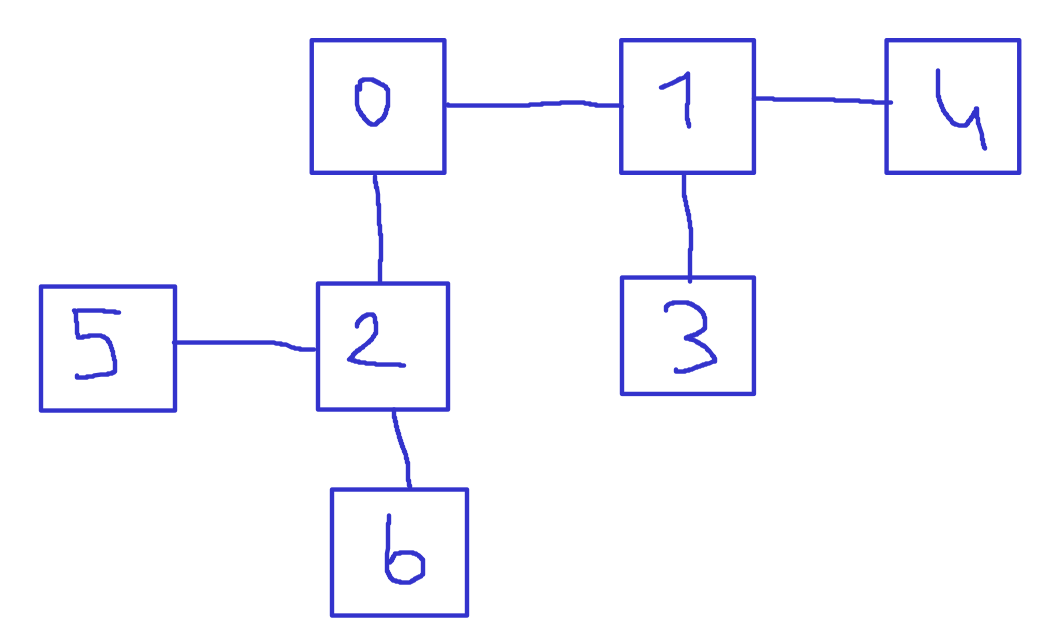
\includegraphics[width=0.5\textwidth]{images/bfs.png}
    \caption{}
\end{figure}

\begin{lstlisting}[language=Python]
from collections import deque

def breath_first_search(graph, start):
    visited = [False] * len(graph)
    queue = deque([start])
    visited[start] = True
    while queue:
        current_node = queue.popleft()
        print(current_node, end=" ")
        for neighbor in graph[current_node]:
            if not visited[neighbor]:
                queue.append(neighbor)
                visited[neighbor] = True


graph = {0: [1, 2], 1: [0, 3, 4], 2: [0, 5, 6],
         3: [1], 4: [1], 5: [2], 6: [2]}
breath_first_search(graph, start=1)
# 1 0 3 4 2 5 6 
\end{lstlisting}

\newpage

\subsection{Depth-First Search (DFS)}

Depth-First Search (DFS), bir graf ya da ağaç üzerindeki düğümleri derinlik öncelikli ziyaret eden bir arama algoritmasıdır. DFS, bir dalı tamamen keşfedene kadar derinlemesine iner, geri döner ve diğer dallara aynı işlemi uygular. Yani, her düğümün olabildiğince derinine inip keşfetmek temel stratejisidir. DFS, önce bir düğümden olabildiğince derine iner, bir yol tıkanırsa (yeni düğüm kalmazsa) geri dönerek diğer yolları keşfeder. Eğer graf sonluysa, DFS mutlaka bir çözüm bulur. Ancak, döngüler içeren sonsuz graflarda çözüm bulamayabilir. DFS en kısa yolu bulmayı garanti etmez, bu nedenle optimal değildir. Graf, $V$ düğüm ve $E$ kenardan oluşuyorsa, zaman karmaşıklığı $O(V + E)$'dir. Yani her düğüm bir kez ziyaret edilir ve her kenar bir kez işlenir.

\subsubsection{Python Kodu}

\begin{figure}[h]
    \centering
    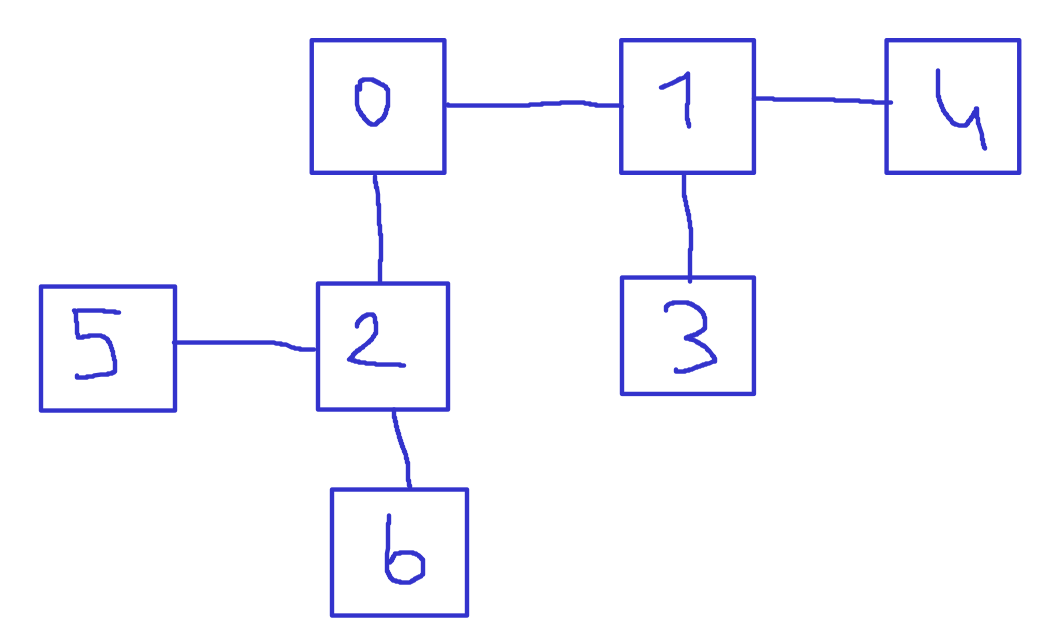
\includegraphics[width=0.5\textwidth]{images/dfs.png}
    \caption{}
\end{figure}

\begin{lstlisting}[language=Python]
def depth_first_search(graph, start):
    visited = [False] * len(graph)
    stack = [start]
    while stack:
        current_node = stack.pop()
        if not visited[current_node]:
            visited[current_node] = True
            print(current_node, end=" ")
            for neighbor in reversed(graph[current_node]):
                stack.append(neighbor)

graph = {0: [1, 2], 1: [0, 3, 4], 2: [0, 5, 6],
         3: [1], 4: [1], 5: [2], 6: [2]}
depth_first_search(graph, start=1)
# 1 0 2 5 6 3 4 
\end{lstlisting}

\newpage

\subsection{Uniform Cost Search (UCS)}

Uniform Cost Search (UCS), bir BFS türüdür, ancak farkı, kenar ağırlıklarını dikkate alarak en düşük maliyetli yolu bulmasıdır. UCS, her zaman en düşük maliyetli düğümü genişleterek hedefe ulaşmaya çalışır. UCS, her adımda en düşük maliyetli düğümü genişletir. Her kenarın ağırlığı (maliyeti) varsa, BFS'den farklı olarak bu ağırlıkları hesaba katar. Eğer çözüm varsa, UCS onu mutlaka bulur. UCS, en düşük maliyetli çözümü bulur, yani optimaldir. Düğüm genişletme işlemi her zaman maliyeti en düşük düğümle yapılır, böylece en kısa yol garantilenir. UCS'in zaman karmaşıklığı, genişletilen düğümlerin sayısına bağlıdır. En kötü durumda, her düğüm genişletildiğinde maliyet kontrol edilir, bu da $O((V + E) \text{log}V)$'dir, burada $V$ düğüm sayısı ve $E$ kenar sayısıdır.

\subsubsection{Python Kodu}

\begin{figure}[h]
    \centering
    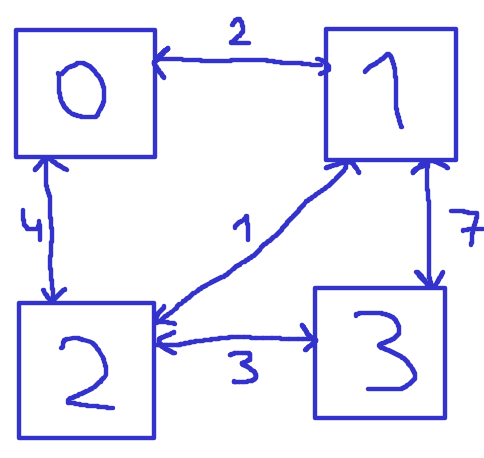
\includegraphics[width=0.5\textwidth]{images/ucs.png}
    \caption{}
\end{figure}

\begin{lstlisting}[language=Python]
import heapq

def uniform_cost_search(graph, start, goal):
    priority_queue = [(0, start)]
    visited = [False] * len(graph)
    cost_so_far = [float("inf")] * len(graph)
    cost_so_far[start] = 0
    while priority_queue:
        current_cost, current_node = heapq.heappop(priority_queue)
        if current_node == goal:
            return current_cost

        if visited[current_node]:
            continue

        visited[current_node] = True
        for neighbor, cost in graph[current_node]:
            new_cost = current_cost + cost
            if new_cost < cost_so_far[neighbor]:
                cost_so_far[neighbor] = new_cost
                heapq.heappush(priority_queue, (new_cost, neighbor))

    return float("inf")

graph = {0: [(1, 2), (2, 4)], 1: [(0, 2), (2, 1), (3, 7)], 
         2: [(0, 4), (1, 1), (3, 3)], 3: [(1, 7), (2, 3)]}
uniform_cost_search(graph, start=0, goal=3) # 6
\end{lstlisting}

\newpage

\subsection{Depth-Limited Search (DLS)}

Depth-Limited Search (DLS), bir çeşit DFS algoritmasıdır, ancak önceden belirlenmiş bir derinlik sınırı ile çalışır. Bu sınır, algoritmanın maksimum kaç derinlik seviyesine kadar arama yapacağını belirler. Eğer sınır aşılırsa, arama daha fazla derine gitmeden geri döner. DLS, DFS'in sonsuz derinliğe sahip grafiklerde veya ağaçlarda sonsuz döngüye girmesini engellemek için kullanılır. Eğer derinlik sınırı hedef düğümün seviyesinden küçükse, DLS hedefi bulamayabilir, bu nedenle tam değildir. Ancak, doğru sınır seçildiğinde tam olabilir. DLS, maliyet fonksiyonunu dikkate almaz, bu yüzden optimal değildir. Zaman karmaşıklığı, en kötü durumda $O(b^L)$'dir. Burada $b$ bir düğümün sahip olabileceği maksimum çocuk sayıdır ve $L$ derinlik sınırıdır.

\subsubsection{Python Kodu}

\begin{figure}[h]
    \centering
    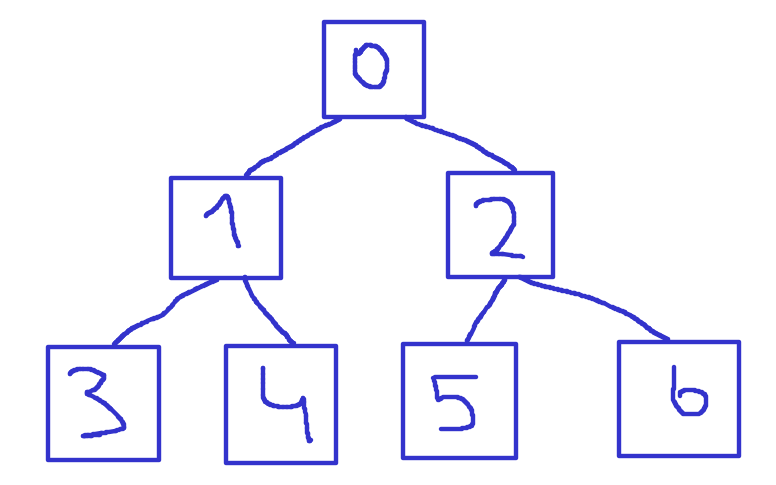
\includegraphics[width=0.5\textwidth]{images/dls.png}
    \caption{}
\end{figure}

\begin{lstlisting}[language=Python]
def reconstruct_path(stack, start, goal):
    path = [goal]
    while stack:
        node, _ = stack.pop()
        if node in path:
            break
        path.append(node)
    path.reverse()
    return path

def depth_limited_search(graph, start, goal, limit):
    stack = [(start, 0)]
    visited = set()

    while stack:
        node, depth = stack.pop()
        if node not in visited:
            visited.add(node)
            if node == goal:
                return reconstruct_path(stack, start, goal)
            if depth < limit:
                for neighbor in graph[node]:
                    stack.append((neighbor, depth + 1))
    return None

graph = {0: [1, 2], 1: [3, 4], 2: [5, 6], 
         3: [], 4: [], 5: [], 6: []}
depth_limited_search(graph, start=0, goal=6, limit=2)
# [1, 5, 6]
\end{lstlisting}

\newpage

\subsection{Iterative Deepening Depth-First Search (IDDFS)}

Iterative Deepening Depth-First Search (IDDFS), bir derinlik-sınırlı arama stratejisidir. Ancak bu stratejide, derinlik sınırı kademeli olarak artırılır. Yani, belirli bir derinlik sınırıyla başlar ve o sınırla bir DFS yapar. Eğer hedef bulunamazsa, sınır bir artırılır ve tekrar DFS yapılır. Bu işlem, hedef bulunana kadar devam eder. IDDFS, hem DFS hem de BFS yöntemlerinin avantajlarını birleştirir: DFS gibi az bellek kullanır. BFS gibi en kısa çözümü bulabilir (optimaldir) ve tamdır. IDDFS, sonlu bir ağaçta ya da grafikte hedef düğümün bulunduğu derinliğe kadar tüm seviyeleri sırasıyla araştırdığı için tamdır. IDDFS, en kısa çözüm yolunu bulur, bu yüzden BFS gibi optimaldir. Zaman karmaşıklığı, en kötü durumda $O(b^L)$'dir. Burada $b$ bir düğümün sahip olabileceği maksimum çocuk sayıdır ve $L$ derinlik sınırıdır.

\subsubsection{Python Kodu}

\begin{figure}[h]
    \centering
    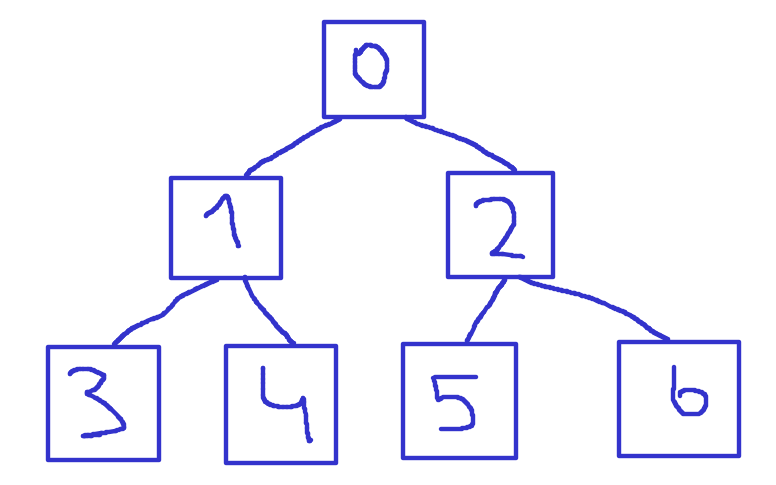
\includegraphics[width=0.5\textwidth]{images/iddfs.png}
    \caption{}
\end{figure}

\begin{lstlisting}[language=Python]
def iterative_deepening_dfs(graph, start, goal, limit):
    for depth in range(limit + 1):
        stack = [(start, 0)]
        visited = set()

        while stack:
            node, current_depth = stack.pop()
            if node not in visited:
                visited.add(node)
                if node == goal:
                    return depth
                if current_depth < depth:
                    for neighbor in graph[node]:
                        stack.append((neighbor, current_depth + 1))

    return None

graph = {0: [1, 2], 1: [3, 4], 2: [5, 6], 
         3: [], 4: [], 5: [], 6: []}
iterative_deepening_dfs(graph, start=0, goal=6, limit=3)
# 2
\end{lstlisting}

\newpage

\subsection{Bidirectional Search}

Bidirectional Search, hedef arama problemlerinde arama işlemini iki yönde aynı anda başlatan bir algoritmadır. Arama, hem başlangıç noktasından hedefe doğru ileri yönde yapılır, aynı zamanda hedeften başlangıç noktasına doğru geri yönde yapılır. Bidirectional Search, iki yönlü aramayı aynı anda çalıştırır. İleri yönde başlangıç düğümünden başlarken, geri yönde hedef düğümünden başlar. Her iki arama da genişlettikleri düğümleri birer veri yapısında tutar. Düğümlerden biri diğerinin genişlettiği düğümlerle kesiştiğinde, arama sona erer. Bu kesişim, çözümün bulunduğunu gösterir. Eğer bir çözüm varsa, bidirectional search kesinlikle bu çözümü bulur. Bu nedenle tamdır. İki yönlü arama, en kısa yolu bulur. Düğümler arasında aynı maliyete sahip yollar varsa optimal bir çözüme ulaşır. Zaman karmaşıklığı $O(b^{\frac{d}{2}})$'dir. Burada $b$ dallanma faktörü, $d$ hedef düğümün derinliğidir.

\subsubsection{Python Kodu}

\begin{figure}[h]
    \centering
    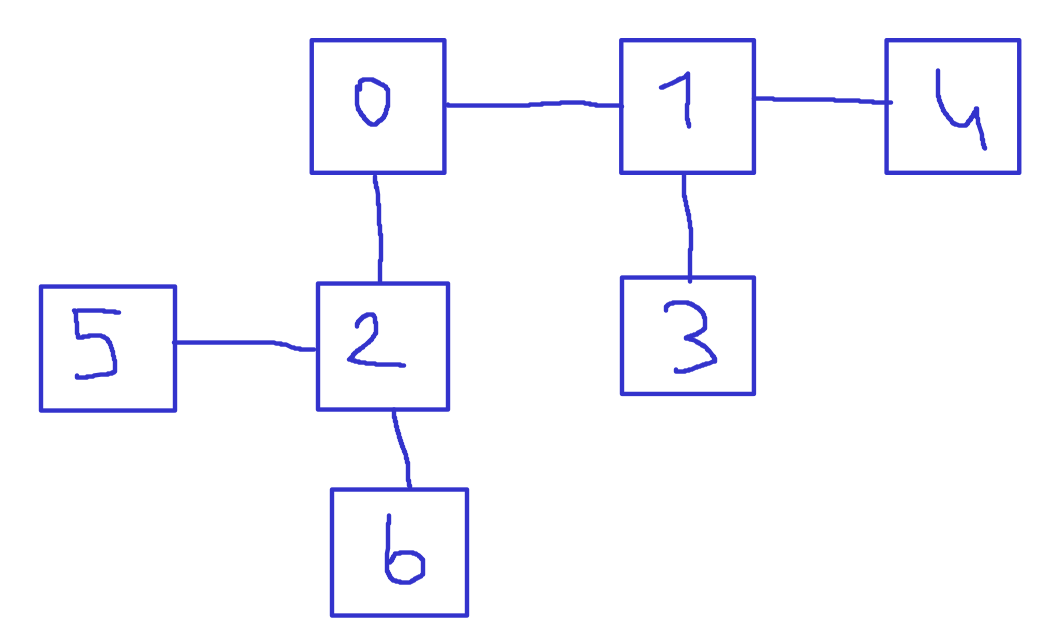
\includegraphics[width=0.5\textwidth]{images/bidirectional.png}
    \caption{}
\end{figure}

\begin{lstlisting}[language=Python]
from collections import deque

def bidirectional_search(graph, start, goal):
    start_queue = deque([start])
    goal_queue = deque([goal])
    start_visited = {start}
    goal_visited = {goal}

    while start_queue and goal_queue:
        current_node = start_queue.popleft()
        for neighbor in graph[current_node]:
            if neighbor in goal_visited:
                return True
            if neighbor not in start_visited:
                start_visited.add(neighbor)
                start_queue.append(neighbor)

        current_node = goal_queue.popleft()
        for neighbor in graph[current_node]:
            if neighbor in start_visited:
                return True
            if neighbor not in goal_visited:
                goal_visited.add(neighbor)
                goal_queue.append(neighbor)

    return False

graph = {0: [1, 2], 1: [0, 3, 4], 2: [0, 5, 6],
         3: [1], 4: [1], 5: [2], 6: [2]}
bidirectional_search(graph, start=0, goal=6)
# True
\end{lstlisting}

\newpage

\subsection{Best First Search}

Best First Search, her adımda en iyi görünen (en az maliyetli veya hedefe en yakın) düğümü genişletir. Bu seçim için bir heuristic (sezgisel) kullanılır. Sezgisel, düğümlerin hedefe ne kadar yakın olduğunu tahmin eden bir fonksiyondur ve algoritma her adımda bu tahmini en küçük olan düğümü genişletir. Sezgisel bir fonksiyonla düğümlerin hedefe yakınlığı tahmin edilerek seçim yapılır. Zaman karmaşıklığı $O(b^d)$'dir. Burada $b$ dallanma faktörü, $d$ hedef düğümün derinliğidir.

\subsubsection{Python Kodu}

\begin{figure}[h]
    \centering
    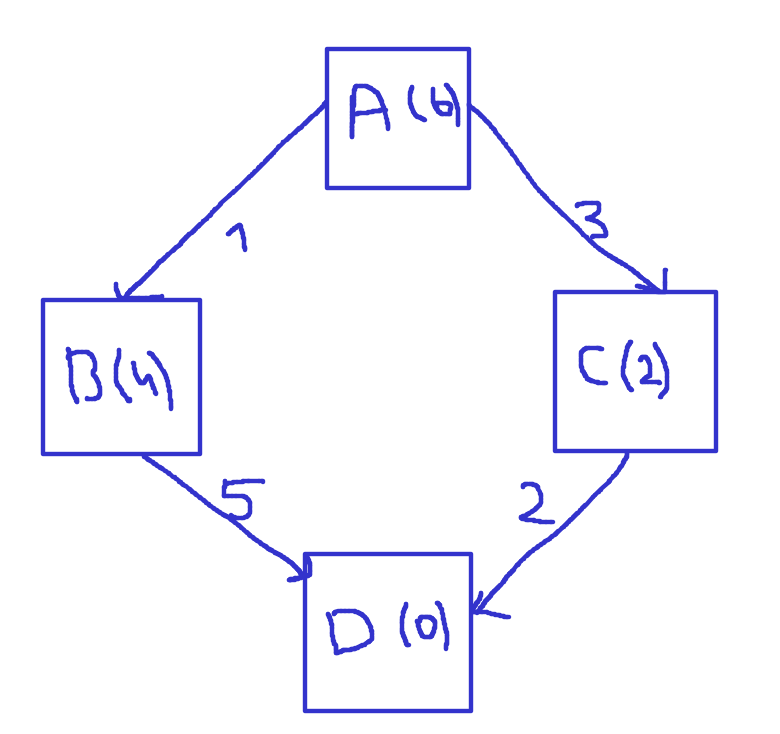
\includegraphics[width=0.5\textwidth]{images/best_first_search.png}
    \caption{}
\end{figure}

\begin{lstlisting}[language=Python]
import heapq

class Node:
    def __init__(self, name, heuristic):
        self.name = name
        self.heuristic = heuristic
        self.neighbors = []

    def add_neighbor(self, neighbor, cost):
        self.neighbors.append((neighbor, cost))

    def __lt__(self, other):
        return self.heuristic < other.heuristic

def best_first_search(start, goal):
    open_list = []
    heapq.heappush(open_list, start)
    visited = set()
    while open_list:
        current_node = heapq.heappop(open_list)
        if current_node.name == goal.name:
            return True
        
        visited.add(current_node)
        for neighbor, cost in current_node.neighbors:
            if neighbor not in visited:
                heapq.heappush(open_list, neighbor)
    
    return False

A = Node("A", 6)
B = Node("B", 4)
C = Node("C", 2)
D = Node("D", 0)
A.add_neighbor(B, 1)
A.add_neighbor(C, 3)
B.add_neighbor(D, 5)
C.add_neighbor(D, 2)
best_first_search(start=A, goal=D)
# True
\end{lstlisting}

\newpage

\subsection{A* Search}
A* Search, graf tabanlı problemlerde en kısa yolu bulmak için kullanılan güçlü bir informed search (bilgilendirilmiş arama) algoritmasıdır. Bu algoritma, hem en kısa yolu bulmayı hem de arama sürecini hızlandırmayı amaçlar. A* Search, iki temel bileşen kullanarak düğümlerin genişletilmesini yönetir:

\begin{itemize}
    \item $g(n)$: Başlangıç düğümünden $n$ düğümüne kadar olan maliyet (gerçek maliyet).
    \item $h(n)$: $n$ düğümünden hedefe olan tahmini maliyet (heuristic).
\end{itemize}

A* Search, her adımda düğümleri $f(n) = g(n) + h(n)$ maliyetine göre genişletir. Bu, algoritmanın her adımda hedefe en kısa yoldan gitmesini sağlar. A* Search, uygun bir heuristic kullanıldığında her zaman hedefi bulur, yani tamdır. A* algoritması, eğer heuristic tutarlı (consistent) ya da aşağılayıcı (admissible) ise en kısa yolu bulur. Aşağılayıcı heuristic, hiçbir zaman gerçek maliyeti aşmaz. Zaman karmaşıklığı, en kötü durumda $O(b^d)$'dir. Burada $b$ dallanma faktörü, $d$ hedef düğümün derinliğidir.

\subsubsection{Python Kodu}

\begin{figure}[h]
    \centering
    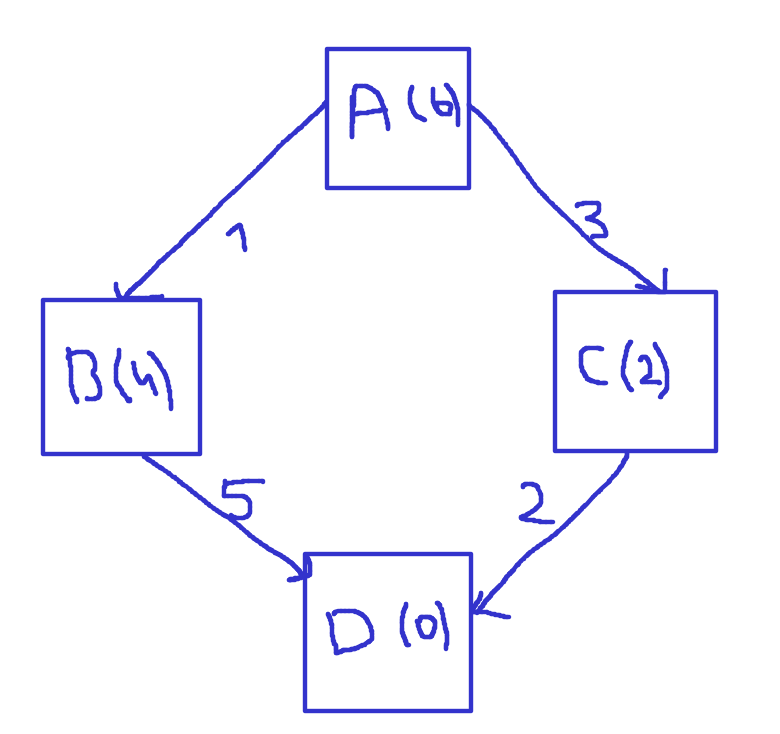
\includegraphics[width=0.5\textwidth]{images/a_start_search.png}
    \caption{}
\end{figure}

\begin{lstlisting}[language=Python]
class Node:
    def __init__(self, name, heuristic):
        self.name = name
        self.heuristic = heuristic
        self.neighbors = []

    def add_neighbor(self, neighbor, cost):
        self.neighbors.append((neighbor, cost))

    def __lt__(self, other):
        return self.heuristic < other.heuristic

def a_star_search(start, goal):
    g_values = {start: 0}
    open_list = [(start, start.heuristic)]
    visited = set()
    while open_list:
        current_node, _ = min(open_list, key=lambda x: x[1])
        open_list.remove((current_node, _))
        if current_node.name == goal.name:
            return True

        visited.add(current_node)
        for neighbor, cost in current_node.neighbors:
            if neighbor in visited:
                continue 

            new_g = g_values[current_node] + cost
            if neighbor not in g_values or new_g < g_values[neighbor]:
                g_values[neighbor] = new_g
                f_value = new_g + neighbor.heuristic
                open_list.append((neighbor, f_value))

    return False

A = Node("A", 6)
B = Node("B", 4)
C = Node("C", 2)
D = Node("D", 0)
A.add_neighbor(B, 1)
A.add_neighbor(C, 3)
B.add_neighbor(D, 5)
C.add_neighbor(D, 2)
a_star_search(start=A, goal=D)
# True
\end{lstlisting}

\newpage

\subsection{Dijsktra's Algorithm}

Dijkstra'nın algoritması, bir kaynaktan bir hedefe veya bir kaynaktan diğer tüm düğümlere en kısa yolları bulan bir greedy (açgözlü) algoritmadır. Yönlü ve pozitif ağırlıklı grafiklerde kullanılır. Temel amacı, bir başlangıç düğümünden diğer düğümlere en kısa yolu bulmaktır. Algoritma sadece pozitif ağırlıklı kenarları olan grafiklerde çalışır. Negatif ağırlıklar için kullanılmaz (Bellman-Ford algoritması negatif ağırlıklar için daha uygundur). Her adımda, en kısa yolu keşfetmek için açgözlü bir seçim yapılır. Yani, şu ana kadar bulunan en kısa mesafeli düğüm seçilir ve genişletilir.

\begin{enumerate}
    \item Kaynak düğümün başlangıç mesafesini sıfır yapılır ve diğer tüm düğümler için mesafeleri sonsuz olarak ayarlanır.
    \item Her düğüm için en kısa mesafe güncellenir ve en kısa mesafeye sahip düğümü seçilerek ilerlenir.
    \item Seçilen düğümden komşu düğümlere giden yolların maliyeti güncellenir.
    \item Tüm düğümler ziyaret edilene kadar bu işlemi tekrarlanır.
\end{enumerate}

\newpage

\subsection{Bellman-Ford Algorithm}

En kısa yolları bulmada kullanılır ve negatif ağırlıkların olduğu durumlarda tercih edilir. Bu algoritma, negatif ağırlıklı döngüleri de algılayabilir, bu da Dijkstra'nın algoritmasından önemli bir farktır. Ancak, Dijkstra algoritmasından daha yavaştır. ellman-Ford algoritması, negatif ağırlıklı kenarları olan grafikleri işleyebilir ve bu grafikleri doğru bir şekilde çalıştırabilir.  Grafikte negatif ağırlıklı döngüler (bir döngü boyunca toplam ağırlık negatif olan kenarlar) varsa, Bellman-Ford bunu tespit edebilir. Yönlendirilmiş veya yönlendirilmemiş grafiklerde çalışabilir.

\begin{enumerate}
    \item Başlangıç düğümünün mesafesi sıfır yapılır, diğer tüm düğümler için mesafeleri sonsuz olarak başlatılır.
    \item Tüm kenarlar $V - 1$ kez kontrol edilir. Her kontrol sırasında, hedef düğüme ulaşmanın daha kısa bir yolu varsa mesafe güncellenir.
    \item Eğer $V - 1$ iterasyondan sonra hala mesafeler güncelleniyorsa negatif döngü vardır.
\end{enumerate}

\newpage

\subsection{Floyd-Warshall Algorithm}

Floyd-Warshall algoritması, bir grafikteki tüm düğümler arasındaki en kısa yolları bulmak için kullanılan bir dinamik programlama algoritmasıdır. Bu algoritma, grafikteki her düğüm çiftinin arasındaki en kısa yolu bulur ve hem pozitif hem de negatif ağırlıklı kenarları destekler. Negatif ağırlıklı döngülerin olup olmadığını da tespit edebilir. Hem ağırlıklı hem de yönlendirilmiş grafiklerde çalışır.

\begin{enumerate}
    \item İlk başta, grafiğin uzaklık matrisi oluşturulur. Başlangıçta, her düğüm çiftinin arasındaki mesafe grafik üzerindeki kenar ağırlıkları ile başlatılır. Eğer düğümler arasında bir kenar yoksa mesafe sonsuz olarak başlatılır.
    \item Her düğüm, ara düğüm olarak kullanılarak, diğer düğüm çiftlerinin mesafeleri bu düğüm üzerinden geçip daha kısa hale gelip gelmediği kontrol edilir.
    \item Tüm düğümler için en kısa mesafeler hesaplandıktan sonra sonuç matrisi döndürülür.
\end{enumerate}

\newpage

\subsection{Kruskal's Algorithm}

Kruskal Algoritması, ağırlıklı ve bağlantılı bir grafikte Minimum Spanning Tree (MST) (minimum öbek ağaç) oluşturmak için kullanılan bir greedy algoritmadır. MST, bir grafikteki tüm düğümleri birbirine bağlayan minimum toplam ağırlıklı kenarlar kümesini temsil eder. Kruskal algoritması, ağacın minimum ağırlıklı kenarlarını seçerek, döngü oluşturmadan tüm düğümleri birbirine bağlayan bir alt grafik oluşturur. Algoritma, her adımda mevcut en düşük ağırlıklı kenarı seçerek ilerler. Her kenar eklendiğinde bir döngü oluşup oluşmadığı kontrol edilir. Döngü oluşursa kenar eklenmez. 

\begin{enumerate}
    \item Tüm kenarlar, ağırlıklarına göre artan şekilde sıralanır.
    \item Sırayla en küçük ağırlıklı kenarlar seçilir ve bu kenar eklendiğinde bir döngü oluşup oluşmadığı kontrol edilir.
    \item Döngü oluşumunu kontrol etmek için Union-Find veri yapısı kullanılır. Aynı kümeye ait olmayan iki düğüm birleştirilir.
    \item Tüm düğümler bağlantılı hale gelene veya seçilen kenar sayısı $V - 1$ olana kadar kenarlar eklenmeye devam edilir.
\end{enumerate}

\newpage

\subsection{Prim's Algorithm}

Prim’s Algoritması, ağırlıklı bir grafikte Minimum Spanning Tree (MST) (minimum öbek ağaç) oluşturmak için kullanılan bir greedy algoritmadır. Bu algoritma, belirli bir başlangıç düğümünden başlar ve her adımda, mevcut ağaca en yakın olan en düşük ağırlıklı kenarı seçerek ilerler. Bu sayede tüm düğümleri kapsayan bir ağ oluşturulur. Algoritma, belirli bir düğümden başlar ve her adımda ağaca en az ağırlıkla bağlanabilecek komşu düğümü seçer. Her adımda döngü oluşturulmadan yeni bir kenar eklenir. MST her adımda genişleyerek daha fazla düğüm kapsar. Her adımda en düşük ağırlıklı kenar seçilir.

\begin{enumerate}
    \item Rastgele bir düğüm seçilir.
    \item Her adımda mevcut ağaca en az ağırlıklı kenar eklenir.
    \item Yeni kenarın eklenmesi döngü oluşturmamalıdır.
    \item Tüm düğümler eklenene kadar işlem devam eder.
\end{enumerate}

\newpage

\subsection{Boruvka's Algorithm}

Boruvka'nın Algoritması, minimum öbek ağaç (Minimum Spanning Tree, MST) oluşturmak için kullanılan en eski algoritmalardan biridir. Bu algoritma, başlangıçta her düğümü kendi ağacı olarak kabul eder ve her adımda her ağaç için en düşük maliyetli kenarı ekleyerek büyüyen bir MST oluşturur. Borůvka'nın algoritması, küme tabanlı (component-based) bir yaklaşım kullanarak ilerler. Başlangıçta her düğüm bir küme oluşturur ve her adımda her küme, kendisine en düşük maliyetli kenarı ekleyerek başka bir kümeyle birleşir. Algoritma, her adımda birden fazla kenarı ekleyebildiği için paralel işlemeye uygundur. Her küme, kendisine en yakın düğümü bulur ve kenarı ekler. Bu süreç, tüm kümeler tek bir MST oluşturana kadar devam eder. Algoritma, her adımda mevcut kümeye en düşük maliyetli kenarı ekler.

\begin{enumerate}
    \item Her düğüm başlangıçta bağımsız bir küme olarak kabul edilir.
    \item Her adımda, her küme için en yakın düğümle olan en düşük maliyetli kenar seçilir.
    \item Bu kenarlar eklenerek kümeler birleşir.
    \item Tek bir küme (MST) oluşana kadar işlem devam eder.
\end{enumerate}

\newpage

\subsection{Kahn's Algorithm}

Kahn's Algorithm, yönlü bir grafiğin topolojik sıralamasını bulmak için kullanılan bir algoritmadır. Topolojik sıralama, bir DAG (Directed Acyclic Graph) üzerindeki düğümlerin sırasını bulur, bu sırada her kenar $(u, v)$ için $u$, $v$'den önce gelir. Yani, bir düğüme giden her yol önceki düğümden başlar. Bu algoritma, bir işin yapılma sırasını belirlemek veya bağımlılık sıralaması gereken durumlarda kullanılır. Yönlü, döngüsüz grafiğin düğümlerini, her düğümün yalnızca tüm bağımlılıkları çözüldükten sonra yerleştirilebileceği sıraya sokar. Algoritma, sadece döngüsüz yönlü grafiklerde uygulanabilir. Eğer grafik döngü içeriyorsa, topolojik sıralama yoktur. Her düğümün giriş derecesi (in-degree) hesaplanır, yani düğüme gelen kenarların sayısı. Giriş derecesi sıfır olan düğümler sıraya alınır.

\begin{enumerate}
    \item Tüm düğümlerin giriş dereceleri hesaplanır.
    \item Giriş derecesi sıfır olan düğümler bir sıraya eklenir.
    \item Bu düğümler sırayla işlenip grafikten çıkarılır. Grafikten çıkarılırken, bu düğümlerden giden kenarlar da kaldırılır ve bu kenarların hedef düğümlerinin giriş dereceleri azaltılır.
    \item Sıra boşalana ve tüm düğümler işlenene kadar devam edilir.
    \item Eğer işlenmeyen düğüm kalmımşsa, grafikte döngü vardır ve topolojik sıralam yapılmaz.
\end{enumerate}

\newpage

\subsection{Union-Find Algorithm}

Union-Find Algorithm (aynı zamanda Disjoint Set Union (DSU) veya Find-Union Algorithm olarak da bilinir), kümeler üzerinde etkili bir şekilde işlem yapmak için kullanılan bir veri yapısıdır. Bu algoritma, belirli kümelerde elemanların hangi kümeye ait olduğunu bulma (Find) ve iki kümenin birleşimini yapma (Union) işlemlerini hızlı bir şekilde gerçekleştirmek için kullanılır. Union-Find algoritması grafikte bağlantılı bileşenleri bulmak, Kruskal algoritması gibi minimum kovan ağacı (MST) algoritmalarında döngüleri tespit etmek ve çeşitli küme işlemlerini gerçekleştirmek için kullanılır.

\begin{enumerate}
    \item bir elemanın hangi kümeye ait olduğunu bulunur. Bu işlem, elemanın bağlı olduğu kök düğümü (temsilcisi) bulur. Tüm elemanlar bir kök düğüm tarafından temsil edilir.
    \item İki kümenin birleşimini gerçekleştirir. İki elemanın kök temsilcilerini bulur ve onları birleştirir.
    \item Find işlemi sırasında, her elemanı doğrudan kök düğümüne bağlamak için yol sıkıştırması yapılır. Bu, daha sonraki işlemleri hızlandırır.
    \item Union işlemi sırasında, daha küçük rütbeye sahip olan küme, daha büyük rütbeye sahip olan kümeye bağlanır. Bu, ağacın boyutunu küçük tutmak için kullanılır ve Find işlemini hızlandırır.
\end{enumerate}

\newpage

\subsection{Kosaraju's Algorithm}

Kosaraju's Algorithm, yönlü bir grafikte güçlü bağlı bileşenleri (Strongly Connected Components, SCC) bulmak için kullanılan etkili bir algoritmadır. Bir grafik içindeki bir bileşen, bileşen içindeki herhangi bir düğümden diğer herhangi bir düğüme ulaşılabilmesi durumunda "güçlü bağlı bileşen" olarak adlandırılır. Kosaraju'nun algoritması, iki derinlemesine arama (DFS) işlemiyle çalışır. 

\begin{enumerate}
    \item Grafikte tüm düğümler üzerinde DFS yaparak, düğümlerin bitiş zamanlarını hesaplar ve düğümleri bir yığın içine yerleştirir. Bu adımda grafiğin sadece düğümleri ve kenarları gezilir.
    \item Grafiğin transpozu (tersi) alınır. Bu adımda tüm kenarların yönü ters çevirilir.
    \item Yığından teker teker düğümleri alarak, ters grafikte DFS yapılır. Bu DFS işlemi sırasında her DFS çağrısı ile güçlü bağlı bileşen bulunur.
\end{enumerate}

\newpage

\subsection{Tarjan's Algorithm}

Tarjan's Algorithm, yönlü bir grafikte güçlü bağlı bileşenleri (Strongly Connected Components, SCC) bulmak için kullanılan bir başka etkili algoritmadır. Bu algoritma, DFS (Depth First Search) kullanarak tüm düğümleri ziyaret eder ve bir düğümün ait olduğu SCC'yi, o düğüm DFS'de ziyaret edilirken bulur. Tarjan’ın algoritması, düğümleri bir yığın kullanarak izler ve düğümün DFS’te keşfedilme zamanlarını ve geri dönülebilecek en düşük seviyeyi hesaplar. Algoritma, SCC'leri tespit etmek için yığın kullanır. Her düğüm, DFS sırasında geri dönebileceği en düşük bağlantı değerine sahiptir. Bu değer, düğümün hangi SCC'ye ait olduğunu belirlemek için kullanılır. Düşük bağlantı değeri ve keşif zamanı kullanılarak DFS sırasında geri çekilme yapılır.

\begin{enumerate}
    \item Algoritma, her düğümden bir DFS işlemi başlatarak tüm düğümleri ziyaret eder.
    \item Her düğüm için bir keşif zamanı atanır. Ayrıca her düğümün bağlı olduğu SCC'nin tespiti için düşük bağlantı değeri (low-link value) hesaplanır.
    \item Algoritma, DFS sırasında düğümleri bir yığında tutar. Eğer bir düğüm, kendi SCC'sinin kök düğümü ise, yığından bu SCC'yi çıkartarak güçlü bağlı bileşeni oluşturur.
\end{enumerate}

\newpage

\subsection{Ford-Fulkerson Algorithm}

Ford-Fulkerson Algoritması, bir akış ağındaki maksimum akışı bulmak için kullanılan bir algoritmadır. Bir kaynak düğümü (source) ile hedef düğüm (sink) arasında, kenar kapasitelerine saygı göstererek maksimum akışı bulmayı hedefler. Bu algoritma, artırılabilir yollar bularak bu yollar üzerinden akış değerlerini günceller ve sonucu elde eder. Algoritma, artan bir yol bulduğu sürece akışı artırmaya devam eder. Algoritma, her adımda orijinal grafiğin bir artık grafini oluşturur. Bu grafikte, mevcut kapasitelere göre akışlar hesaplanır.

\begin{enumerate}
    \item Tüm kenarlarda başlangıçta sıfır akış atanır.
    \item Kaynak düğümünden hedef düğüme giden ve artırılabilir kapasiteye sahip bir yol bulunur. Bu yol DFS veya BFS kullanılarak bulunabilir.
    \item Bu artırılabilir yol üzerindeki tüm kenarlar üzerinden maksimum artırılabilir kapasite kadar akış eklenir. Ayrıca, her artırma işlemiyle birlikte ters yöndeki akışlar da güncellenir.
    \item Artırılabilir bir yol bulunamadığında algoritma durur. Bulunan maksimum akış, bu noktada elde edilen toplam akış değeridir.
\end{enumerate}

\newpage

\subsection{Edmonds-Karp Algorithm}

Edmonds-Karp Algoritması, Ford-Fulkerson yönteminin bir genişletmesidir ve ağlarda maksimum akışı bulmak için kullanılır. Bu algoritma, artan yolları bulmak için BFS (Breadth-First Search) kullanır. BFS, her seferinde en kısa artan yolu bulmaya çalışarak algoritmanın çalışmasını garanti eder. Bu sayede, Ford-Fulkerson algoritmasının performansı iyileştirilir ve zaman karmaşıklığı daha belirgindir. 

\begin{enumerate}
    \item Kaynak düğümünden hedef düğüme sıfır akışla başlanır.
    \item BFS kullanarak kaynak düğümünden hedef düğüme giden artırılabilir bir yol bulunur.
    \item Bulunan yol üzerinden mümkün olan maksimum akış artırılır ve kenar kapasiteleri güncellenir. Ters yönlü akışlar da hesaba katılır.
    \item Artan bir yol bulunduğu sürece bu işlem tekrarlanır.
    \item Artan bir yol bulunamazsa, algoritma sona erer ve maksimum akış bulunmuş olur.
\end{enumerate}

\newpage

\subsection{Dinic's Algorithm}

Dinic's Algorithm, ağlarda maksimum akış bulmak için kullanılan bir algoritmadır ve Ford-Fulkerson metodunun bir uzantısıdır. Bu algoritma, BFS (Breadth-First Search) ve DFS (Depth-First Search) tekniklerini birleştirerek maksimum akışı daha hızlı bir şekilde bulur. Dinic’s algoritması, özellikle büyük ağlarda ve yüksek dereceli grafiklerde etkili bir şekilde çalışır. 

\begin{enumerate}
    \item Kaynak düğümünden başlayarak BFS kullanarak hedef düğüme ulaşabilecek artan yolları bulur ve katmanlı bir grafik oluşturur.
    \item Katmanlı grafikte DFS ile ilerleyerek artan yolları kullanır ve akışı artırır.
    \item Yeni bir katmanlı grafik oluşturup bu işlemi tekrarlayarak maksimum akışa ulaşılana kadar devam eder.
    \item BFS ile hedef düğüme ulaşamıyorsak, işlem tamamlanır ve maksimum akış bulunmuş olur.
\end{enumerate}

\newpage

\subsection{Push-Relabel Algorithm}

Push-Relabel Algoritması, maksimum akış problemini çözmek için kullanılan bir akış algoritmasıdır. Ağda maksimum akışı bulmak için yerel operasyonlar kullanır ve arttırma yollarını kullanmaz. Bu, Push-Relabel algoritmasını Ford-Fulkerson ve Dinic's gibi artan yol temelli algoritmalardan ayıran temel farktır. Fazla akışın olduğu bir düğümde, akış kenarlar üzerinden hedef düğümlere doğru "itilir" (push). Bir düğümün fazlası varsa, komşu düğümlere itebilir. Eğer bir düğümden itme yapılamıyorsa, o düğüm yeniden etiketlenir ve bir sonraki düğümün seviyesi artırılır. Kaynak düğümünden gelen akışlar, hedefine ulaşana kadar düğümler arasında dolaşır. Bir düğümde fazladan akış olursa, bu fazla akış diğer düğümlere gönderilir.

\begin{enumerate}
    \item Kaynak düğümden tüm komşu düğümlere maksimum kapasitede akış "itilir".
    \item Bir düğümde fazla akış varsa, akış komşu düğümlere doğru itilir. Eğer hedef düğüme giden bir yol varsa, bu yol üzerinden akış artırılır.
    \item Eğer akışın itilebileceği komşu düğüm yoksa, düğümün seviyesi artırılır.
    \item Bu işlemler tekrar edilerek tüm düğümler arasında maksimum akış hesaplanır.
\end{enumerate}

\newpage

\subsection{Greedy Coloring Algorithm}

Greedy Coloring Algoritması (Açgözlü Boyama Algoritması), bir grafın düğümlerini (nodelarını) boyarken, bitişik (komşu) düğümlerin aynı renkte olmamasını sağlamak için kullanılan basit ve sezgisel bir algoritmadır. Bu algoritmanın amacı, grafı minimum sayıda renk ile boyamaktır, ancak açgözlü bir strateji kullanıldığı için her zaman en az renk sayısını garanti etmez. Buna rağmen, pek çok pratik durumda iyi sonuçlar verebilir. Her düğüm sırasıyla ziyaret edilir ve o düğüm için mümkün olan en küçük renk atanır. Her düğüme renk atarken, sadece o anki komşu düğümler göz önünde bulundurulur. En kötü durumda, grafın düğüm derecesinden bir fazlası kadar renk kullanılabilir.

\begin{enumerate}
    \item Her düğüme renk atanmamış olarak başlanır.
    \item İlk düğümü alınır ve ona bir renk atanır.
    \item Her bir sonraki düğüm için, komşularının renkleri kontrol edilir ve kullanılmayan en küçük renkle o düğüm boyanır.
    \item Tüm düğümler boyanana kadar bu işlem tekrar edilir.
\end{enumerate}

\newpage

\subsection{Welsh-Powell Algorithm}

Welsh-Powell Algoritması, bir grafın düğümlerini renklendirme sorununu çözmek için kullanılan bir tür graph coloring (graf renklendirme) algoritmasıdır. Welsh-Powell algoritması, graf düğümlerini belirli bir sıralamaya göre renklendirir ve her bir düğüme, komşularıyla aynı renge sahip olmamasını sağlayacak şekilde en küçük uygun rengi atar. Düğümler sırayla en uygun renkle boyanır, yani mevcut düğüm için kullanılmayan en küçük renk atanır. Düğümler önce derecelerine göre (komşu sayısına göre) azalan bir sırayla sıralanır. En fazla komşusu olan düğüm önce boyanır.

\begin{enumerate}
    \item Grafın tüm düğümleri, derecelerine (komşu sayısı) göre azalan sırayla sıralanır.
    \item Her düğüm için, daha önce boyanmış komşuları ile aynı rengi almayan en küçük renk atanır.
    \item Tüm düğümler boyanana kadar işlem devam eder.
\end{enumerate}

\newpage
\section{Greedy Algorithm}

Greedy Algorithm (Açgözlü Algoritma), kararları o anki duruma göre en iyi görünen seçimi yaparak problemi çözmeye çalışan bir algoritma türüdür. Her adımda, o an için en iyi görünen seçeneği (local optimum) seçer ve bu süreci adım adım devam ettirir. Algoritmanın amacı, sonunda global optimuma ulaşmak olsa da, her zaman doğru çözümü garantileyemez. Her adımda o an için en iyi görünen seçimi yapar. Sonuç olarak, her adımda yerel optimum bulunur. Karar verme aşaması bir defaya mahsustur, yani bir kez verilen karar geri alınmaz (irrevocable). Örneğin;

\begin{itemize}
    \item \textbf{Coin Change Problem}: Belirli bir tutarı en az sayıda bozuk parayla ödeme.
    \item \textbf{Prim's Algorithm}: Minimum ağırlıklı yayılma ağacı (Minimum Spanning Tree) bulma.
    \item \textbf{Kruskal Algorithm}: Minimum ağırlıklı yayılma ağacı bulmak için kullanılan bir başka algoritma.
    \item \textbf{Huffman Coding}: Veri sıkıştırmada kullanılan en optimal bit dizisini üretme algoritması.
    \item \textbf{Dijkstra Algorithm}: Bir grafikte başlangıç düğümünden diğer düğümlere en kısa yolu bulma.
    \item \textbf{Activity Selection Problem}: Zaman çizelgesine en fazla etkinlik eklemek.
    \item \textbf{Fractional Knapsack Problem}: En fazla değer kazanmak için sırt çantasına kısmi nesneler koymak.
\end{itemize}

\newpage

\subsection{Activity Selection Problem}

Activity Selection Problem (Etkinlik Seçimi Problemi), verilen bir zaman diliminde, çakışmayan en fazla sayıda etkinliği seçmeyi amaçlayan bir optimizasyon problemidir. Her etkinlik belirli bir başlangıç ve bitiş zamanı ile tanımlanır ve amaç, bu etkinliklerin çakışmadan, yani bir etkinlik bir diğerinin başlangıç zamanını geçmeden seçilmesidir.

Bu problem, greedy algoritma yaklaşımı ile çözülür. Bu yaklaşımda en kısa bitiş zamanına sahip etkinliği ilk olarak seçmek, ardından seçilen etkinliğin bitiş zamanından sonra başlayan etkinlikleri seçmek gerekir. Bu, her adımda yerel optimumu (en erken biten etkinlik) seçmeyi amaçlar.

\begin{enumerate}
    \item Etkinlikler bitiş zamanlarına göre sıralanır.
    \item İlk etkinlik seçilir (çünkü o en erken biten etkinliktir).
    \item Sonraki etkinliklerden, ilk etkinlikten sonra başlayabilen ve çakışmayan bir etkinlik seçilir.
    \item Bu adım, tüm etkinlikler incelenene kadar tekrarlanır.
\end{enumerate}

\begin{lstlisting}[language=Python]
def activity_selection(activities):
    n = len(activities)
    activities.sort(key=lambda x: x[1])
    selected_activities = [activities[0]]
    last_end_time = activities[0][1]

    for i in range(1, n):
        if activities[i][0] >= last_end_time:
            selected_activities.append(activities[i])
            last_end_time = activities[i][1]

    for activity in selected_activities:
        print(f"Start: {activity[0]}, End: {activity[1]}")
\end{lstlisting}

\newpage

\subsection{Coin Change Problem}

Coin Change Problem (Bozuk Para Problemi), belirli bir para miktarını (tutarı) ödemek için en az sayıda bozuk parayı kullanmayı amaçlayan bir optimizasyon problemidir. Bu problemde, elimizde belirli bozuk para türleri (değerleri) vardır ve hedef, bu bozuk paraları kullanarak belirli bir tutarı oluşturmak için gereken en küçük bozuk para sayısını bulmaktır.

Coin Change Problem genellikle dinamik programlama (Dynamic Programming - DP) yöntemi ile çözülür. Bu yöntem, alt problemlerin çözümünü kullanarak daha büyük problemleri çözer. Bu problemde amaç, her alt toplam için minimum bozuk para sayısını bulmaktır.

\begin{enumerate}
    \item 0 tutarını oluşturmak için 0 bozuk para gerekir.
    \item DP tablosu, her bir tutar için en az kaç bozuk para kullanılması gerektiğini gösterir.
    \item DP tablosu, her bozuk parayı kullanarak mevcut tutarları en küçük bozuk para sayısı ile doldurur.
    \item Verilen tutar için en az bozuk para sayısı, DP tablosunun son elemanında bulunur.
\end{enumerate}

\begin{lstlisting}[language=Python]
def coin_change(coins, amount):
    dp = [float('inf')] * (amount + 1)
    dp[0] = 0
    for coin in coins:
        for i in range(coin, amount + 1):
            dp[i] = min(dp[i], dp[i - coin] + 1)
    
    if dp[amount] == float('inf'):
        return -1
        
    return dp[amount]
\end{lstlisting}

\newpage

\subsection{Fractional Knapsack Problem}

Fractional Knapsack Problem (Kesirli Sırt Çantası Problemi), sırt çantasına eşyalar yerleştirirken, her bir eşyanın bir kısmını alabilmeye izin verildiği bir optimizasyon problemidir. Bu problemde, her eşya bir ağırlık ve değerle tanımlanır ve sırt çantasının kapasitesi belirli bir değere sahiptir. Amaç, sırt çantasını en yüksek değeri elde edecek şekilde doldurmaktır, ancak eşyaların tamamını almak yerine, eşyaların bir kısmını da alabilirsiniz.

Fractional Knapsack, Greedy (Açgözlü) algoritması kullanılarak çözülür. Bu algoritma, her eşyanın değerinin ağırlığına oranını (yani, "değer/ağırlık" oranını) hesaplar ve bu orana göre eşyaları azalan sırayla sıralar. Ardından, eşyaları bu sıralama ile sırt çantasına ekler, ancak çantanın kapasitesi dolana kadar.

\begin{enumerate}
    \item Her eşya için değer/ağırlık oranı hesaplanır.
    \item En yüksek değere sahip olan eşya ilk olarak seçilir.
    \item Çantanın kapasitesini aşmamak için eşyaların tamamı veya bir kısmı çantaya eklenir.
    \item Sırt çantasına konan eşyaların toplam değeri hesaplanır.
\end{enumerate}

\begin{lstlisting}[language=Python]
class Item:
    def __init__(self, value, weight):
        self.value = value
        self.weight = weight
        self.ratio = value / weight

def fractional_knapsack(capacity, items):
    items.sort(key=lambda x: x.ratio, reverse=True)
    total_value = 0.0

    for item in items:
        if capacity == 0:
            break

        if item.weight <= capacity:
            total_value += item.value
            capacity -= item.weight
        else:
            total_value += item.value * (capacity / item.weight)
            capacity = 0

    return total_value
\end{lstlisting}

\newpage
\section{Divide and Conquer Algorithm}

Divide and Conquer (Böl ve Yönet) Algoritmaları, büyük bir problemi daha küçük alt problemlere ayırarak çözme yöntemini benimseyen algoritmalardır. Bu yaklaşım, her bir alt problemi çözmek için aynı yöntemi kullanarak, nihayetinde tüm problemin çözümüne ulaşır. Bölme, problemi küçük parçalara ayırmayı, çözümleme, bu alt problemleri çözmeyi ve birleştirme, çözümleri birleştirerek nihai çözümü elde etmeyi içerir.

\begin{itemize}
    \item \textbf{Bölme (Divide)}: Problem, daha küçük alt problemlere bölünür. Bu adım, problemi daha yönetilebilir hale getirir.
    \item \textbf{Çözümleme (Conquer)}: Alt problemler çözülür. Eğer alt problemler yeterince küçükse doğrudan çözülür, ya da yine aynı yaklaşım uygulanarak alt problemlere bölünür.
    \item \textbf{Birleştirme (Combine)}: Alt problemlerin çözümleri birleştirilerek, orijinal problemin çözümü elde edilir.
\end{itemize}

\newpage

\subsection{Number Factor}

Number Factor (Sayı Çarpanı), bir sayıyı tam bölen pozitif tam sayılardan her birine denir. Bir sayıyı bölen tüm sayılar, o sayının çarpanlarıdır. Bir sayının çarpanlarını bulmak, o sayıyı daha küçük parçalara ayırma işlemidir. Bir sayının çarpanlarını bulmak için o sayıyı 1'den kendisine kadar olan sayılarla böleriz ve bölen sayılar, çarpanlar olarak kabul edilir.

\begin{itemize}
    \item \textbf{Normal Yöntem}: Sayıyı 1'den başlayarak, kendisine kadar olan tüm sayılarla böleriz. Her bölen, sayının bir çarpanı olacaktır.
    \item \textbf{Verimli Yöntem}: Daha hızlı bir yaklaşımda, sadece sayının kareköküne kadar olan sayılarla bölme yapılır. Çünkü her çarpanın eşleşen bir başka çarpanı vardır.
\end{itemize}

\newpage

\subsection{House Robber}

House Robber (Ev Hırsızı) problemi, klasik bir dinamik programlama problemidir. Bu problem, belirli bir sayıdaki evlerden, her evin içinde bir miktar değer (ya da para) bulunduğu ve ardışık evlerin soyulamayacağı bir senaryoda, en yüksek değeri (parayı) çalabilen bir hırsızın nasıl hareket etmesi gerektiğini sorar.

Bir hırsız, bir dizi evin her birinde belirli bir miktarda para olduğunu öğrenir. Ancak, hırsız iki ardışık evi aynı anda soyamaz. Bu nedenle, hırsız bir ev soyarsa, bir sonraki evi soymak zorunda değildir. Amaç, en fazla parayı çalmaktır. Kurallar:

\begin{itemize}
    \item Hırsız ardışık evleri soyamaz.
    \item Hırsız sadece bir seferde bir ev soyar.
    \item Hırsızın hedefi, soymadığı evlerden en yüksek toplam parayı çalmaktır.
\end{itemize}

Bu problem dinamik programlama (DP) kullanarak çözülür. DP yaklaşımında, her evin soyulup soyulmayacağını değerlendiririz ve önceki evlerin sonuçlarını kullanarak çözümü iteratif olarak inşa ederiz. Her evin soygun kararını verirken, önceki evlerin çalınan paralarına bakarız. Eğer $i$. ev soygunu yapılırsa, $(i-1)$'inci evin soygununu yapamayız. $dp[i] = i$'inci eve kadar olan evlerde, en fazla parayı çalma miktarı. Eğer $i$'inci ev soyulursa, $(i-2)$'inci evin sonucu ile $i$'inci evin parasını ekleriz. Eğer $i$'inci ev soyulmazsa, $(i-1)$'inci evin sonucunu alırız.

\begin{lstlisting}[language=Python]
def house_robber(nums):
    if not nums:
        return 0

    if len(nums) == 1:
        return nums[0]

    dp = [0] * len(nums)
    dp[0] = nums[0]
    dp[1] = max(nums[0], nums[1])

    for i in range(2, len(nums)):
        dp[i] = max(dp[i - 1], nums[i] + dp[i - 2])

    return dp[-1]

nums = [2, 7, 9, 3, 1]
house_robber(nums) # 12
\end{lstlisting}

\newpage

\subsection{Convert One String to Another}

"Convert one string to another" (bir stringi diğerine dönüştürme) problemi, bir diziyi (string) başka bir diziye dönüştürmek için gereken işlemleri belirlemeyi amaçlar. Bu, genellikle iki dizi arasındaki edit distance (düzenleme mesafesi) veya Levenshtein mesafesi olarak bilinen bir problemle ilişkilidir. Levenshtein mesafesi, iki dizi arasındaki en küçük düzenleme adımlarını ölçen bir algoritmadır. Bu adımlar, ekleme (insertion), silme (deletion) veya değiştirme (substitution) işlemlerinden birini içerir.

\begin{itemize}
    \item \textbf{Ekleme (Insertion)}: Bir karakteri diziye eklemek.
    \item \textbf{Silme (Deletion)}: Bir karakteri diziden çıkarmak.
    \item \textbf{Değiştirme (Substitution)}: Bir karakteri başka bir karakterle değiştirmek.
\end{itemize}

Çözüm, iki stringin her bir karakteri arasında karşılaştırma yapılacak bir matris oluşturulur. Matrisin her hücresine, ilgili karakterlerin dönüştürülmesi için gereken minimum işlemi yerleştiririz (ekleme, silme, değiştirme). Matrisin en sağ alt hücresindeki değer, iki string arasındaki minimum dönüşüm adımlarını gösterir.

\begin{lstlisting}[language=Python]
def levenshtein_distance(str1, str2):
    n1 = len(str1) + 1
    n2 = len(str2) + 1

    matrix = [[0] * n2 for _ in range(n1)]

    for i in range(n1):
        matrix[i][0] = i

    for j in range(n2):
        matrix[0][j] = j

    for i in range(1, n1):
        for j in range(1, n2):
            if str1[i - 1] == str2[j - 1]:
                cost = 0

            else:
                cost = 1

            matrix[i][j] = min(
                matrix[i - 1][j] + 1,
                matrix[i][j - 1] + 1,
                matrix[i - 1][j - 1] + cost
            )

    return matrix[-1][-1]
\end{lstlisting}

\newpage

\subsection{Zero-One Knapsack Problem}

Bu problem, belirli bir kapasiteye sahip bir sırt çantasına (veya başka bir depolama alanına) çeşitli nesneler (veya eşya) yerleştirme problemini tanımlar. Her nesnenin bir değeri ve ağırlığı vardır ve sırt çantasının kapasitesi sınırlıdır. Amaç; kapasiteyi aşmadan, sırt çantasına yerleştirilebilecek nesnelerin toplam değerini en üst seviyeye çıkarmaktır. Her nesne ya sırt çantasına konur (seçilir) ya da konmaz (seçilmez). Bu yüzden bu problem "0-1" sırt çantası problemi olarak adlandırılır, çünkü her nesne yalnızca iki durumda olabilir: ya seçilir (1), ya da seçilmez (0).

\begin{lstlisting}[language=Python]
def zero_one_knapsack(weights, values, capacity):
    n = len(weights)
    dp = [[0] * (capacity + 1) for _ in range(n + 1)]

    for i in range(1, n + 1):
        for w in range(1, capacity + 1):
            if weights[i-1] <= w:
                dp[i][w] = max(dp[i-1][w], dp[i-1][w - weights[i-1]] + values[i-1])
            else:
                dp[i][w] = dp[i-1][w]
    
    return dp[n][capacity]
\end{lstlisting}

\newpage

\subsection{Longest Common Subsequence (LCS)}

Longest Common Subsequence (LCS), iki dizenin (veya stringin) en uzun ortak alt dizisini (subsequence) bulmaya yönelik bir problemdir. Buradaki "alt dizi" (subsequence), dizenin elemanlarını sırasıyla ama arada başka elemanlar da olabilen bir şekilde seçmeyi ifade eder. Yani, dizenin bazı elemanlarını atlayarak, sırasını koruyarak, diğer dizenin içinde yer alan bir dizi oluşturabilirsiniz.

\begin{lstlisting}[language=Python]
def lcs(X, Y):
    m = len(X)
    n = len(Y)
    
    dp = [[0] * (n + 1) for _ in range(m + 1)]
    
    for i in range(1, m + 1):
        for j in range(1, n + 1):
            if X[i - 1] == Y[j - 1]:
                dp[i][j] = dp[i - 1][j - 1] + 1
            else:
                dp[i][j] = max(dp[i - 1][j], dp[i][j - 1])
    
    return dp[m][n]
\end{lstlisting}

\newpage

\subsection{Longest Palindromic Subsequence (LPS)}

Longest Palindromic Subsequence (LPS), bir dizenin (string) en uzun palindromik alt dizisini bulmaya yönelik bir problemdir. Buradaki "palindromik alt dizi" (subsequence), karakterlerin tersten okunduğunda aynı olan bir dizedir. Verilen bir dize, içindeki karakterlerden sırasıyla (ama ardışık olmak zorunda olmayan) en uzun palindromik alt diziyi bulmamız istenir. Bu alt dizi, tersten okunduğunda da aynı olacak şekilde sıralanmalıdır.

\begin{lstlisting}[language=Python]
def longestPalindromicSubsequence(X):
    n = len(X)
    dp = [[0] * n for _ in range(n)]
    for i in range(n-1, -1, -1):
        for j in range(i, n):
            if X[i] == X[j] and i != j:
                dp[i][j] = dp[i+1][j-1] + 2
            elif i == j:
                dp[i][j] = 1
            else:
                dp[i][j] = max(dp[i+1][j], dp[i][j-1])
    
    return dp[0][:n-1]
\end{lstlisting}

\newpage

\subsection{Minimum Cost to Reach the Last Cell}

Minimum Cost to Reach the Last Cell, bir ızgarada (grid) veya matris üzerinde, başlangıç hücresinden son hücreye kadar gitmek için gereken minimum maliyeti bulmaya yönelik bir problemdir. Bu problem genellikle, her hücreye gitmek için bir maliyetin olduğu, ancak sadece sağa ve aşağıya hareket edebileceğiniz bir ızgara için çözülür. Verilen bir m x n ızgarasında (matris), her hücre bir maliyet değerine sahiptir. Başlangıç noktası genellikle sol üst köşe (0, 0) hücresidir ve hedef noktası sağ alt köşe (m-1, n-1) hücresidir. Bu problemde, sol üst köşeden sağ alt köşeye kadar giderken, her adımda sağa veya aşağıya doğru hareket edebileceğiniz ve her hücrenin bir maliyeti olduğu varsayılır. Amaç, başlangıç hücresinden hedef hücresine ulaşırken toplam maliyetin minimum olmasıdır.

\begin{lstlisting}[language=Python]
def minCostToReachEnd(grid):
    row, col = len(grid), len(grid[0])
    
    dp = [[0] * col for _ in range(row)]
    
    dp[0][0] = grid[0][0]
    
    for j in range(1, col):
        dp[0][j] = dp[0][j-1] + grid[0][j]
    
    for i in range(1, row):
        dp[i][0] = dp[i-1][0] + grid[i][0]
    
    for i in range(1, row):
        for j in range(1, col):
            dp[i][j] = min(dp[i-1][j], dp[i][j-1]) + grid[i][j]
    
    return dp[row-1][col-1]
\end{lstlisting}

\newpage
\section{Dynamic Programming}

Dynamic Programming (DP), bir problemi daha küçük alt problemlere ayırarak çözme yöntemidir. Bu yöntem, bir problemi çözmek için aynı alt problemleri tekrar tekrar çözmek yerine, daha önce çözülen alt problemlerin sonuçlarını saklayarak tekrar hesaplama gereksinimini ortadan kaldırır. DP, genellikle optimizasyon problemlerinde kullanılır ve daha verimli çözümler üretir. Problemin, daha küçük alt problemlere bölünebilmesi gerekir. Bu alt problemler bağımsız olabilir ya da birbiriyle ilişkili olabilir. Problemin çözümü, alt problemlerin çözümlerine dayanıyorsa bu özellik sağlanır. Yani, bir problemin optimal çözümü, alt problemlerin optimal çözümlerinin birleşiminden oluşur. DP, aynı alt problemleri birden fazla kez çözmek zorunda kalır. Bu nedenle, çözülen alt problemler kaydedilerek ilerlenir. Bu özellik, DP'nin verimli olmasını sağlar. DP genellikle iki farklı yaklaşım ile uygulanır:

\begin{itemize}
    \item \textbf{Memoization}: Alt problemlerin çözümleri kaydedilir ve tekrar kullanılır (top-down yaklaşımı).
    \item \textbf{Tabulation}: Tüm alt problemler bir tabloya yerleştirilir ve tablodan en küçükten büyüğe doğru çözüm yapılır (bottom-up yaklaşımı).
\end{itemize}

\newpage

\subsection{Longest Increasing Subsequence (LIS)}

Longest Increasing Subsequence (LIS), bir dizideki ardışık olmayan ancak sıralı en uzun artan alt diziyi bulma problemidir. Yani, verilen bir diziden, sırasını bozmadan, elemanları artan şekilde sıralayarak en uzun alt diziyi elde etmeyi amaçlar. Elemanlar ardışık olmak zorunda değildir, ancak sırasıyla artan olmalıdır.

\begin{lstlisting}[language=Python]
def longest_increasing_subsequence(arr):
    n = len(arr)
    dp = [1] * n 
    
    for i in range(1, n):
        for j in range(i):
            if arr[i] > arr[j]:
                dp[i] = max(dp[i], dp[j] + 1)
    
    return max(dp)
\end{lstlisting}

\newpage

\subsection{Rod Cutting Problem}

Rod Cutting Problem (Çubuk Kesme Problemi), verilen bir çubuğun belirli bir uzunlukta kesilmesiyle en yüksek geliri elde etme problemidir. Çubuğun çeşitli uzunluklara kesilmesi mümkündür ve her uzunluk için bir fiyat belirlenmiştir. Amaç, çubuğu keserek, kesilen parçaların fiyatlarının toplamını maksimize etmektir. Bir çubuğun uzunluğu ve bu uzunluklara karşılık gelen fiyatlar verilmiştir. Çubuk, farklı uzunluklarda kesilebilir ve her bir parçanın bir fiyatı vardır. Çubuğun tamamını tek bir parça halinde satmak yerine, onu daha küçük parçalara kesmek ve bu parçalardan daha fazla gelir elde etmek mümkündür. Kesimlerin sırası önemli değildir. Önemli olan, verilen fiyatlar ile maksimum toplam geliri elde etmektir.

\begin{lstlisting}[language=Python]
def rod_cutting(prices, n):
    dp = [0] * (n + 1)
    for i in range(1, n + 1):
        max_val = -float('inf')
        for j in range(1, i + 1):
            max_val = max(max_val, prices[j - 1] + dp[i - j])
        dp[i] = max_val
    
    return dp[n]
\end{lstlisting}

\newpage

\subsection{Subset Sum Problem}

Subset Sum Problem (Alt Küme Toplamı Problemi), verilen bir sayı kümesinden bazı elemanları seçerek, seçilen elemanların toplamının belirli bir hedef değeri (sum) verip vermediğini bulma problemidir. Yani, bir dizi sayıyı seçip, bu sayılardan toplamı verilen bir hedef değere eşit olan bir alt küme oluşturulup oluşturulamayacağını belirlemeye çalışırız.

\begin{lstlisting}[language=Python]
def subset_sum(arr, target_sum):
    n = len(arr)
    dp = [[False] * (target_sum + 1) for _ in range(n + 1)]
    for i in range(n + 1):
        dp[i][0] = True
    
    for i in range(1, n + 1):
        for j in range(1, target_sum + 1):
            if arr[i - 1] <= j:
                dp[i][j] = dp[i - 1][j] or dp[i - 1][j - arr[i - 1]]
            else:
                dp[i][j] = dp[i - 1][j]
    
    return dp[n][target_sum]
\end{lstlisting}

\newpage
\section{Backtracking}

Backtracking, çözümü doğrulanan bir çözüm uzayında arama yapan ve çözüm bulana kadar çözümleri test eden bir algoritma yöntemidir. Bu yaklaşım genellikle kombinatoryal problemleri çözmek için kullanılır ve çözüm yolu bulunduktan sonra geri adım atılarak başka bir çözüm yolu aranır. Backtracking, genellikle bir karar ağacı üzerinden çözüm arar. Her bir düğümde, bir adım ilerleyerek çözüm yolu oluşturulur. Algoritma, belirli bir çözüm adımını seçer, ardından o adımın geçerli olup olmadığını kontrol eder. Geçerli değilse, geri adım atarak başka bir seçenek dener. Çoğu zaman çözüm arama süreci, çözüme ulaşana kadar adım adım ilerler, ancak geri adım atılması gerektiğinde gereksiz dallardan kaçınır. Ancak, kötü yapılandırılmış problemlerde yüksek zaman karmaşıklığına sahip olabilir. Çözüm yolu, genellikle çözüme ulaşan bir yol bulunana kadar keşfedilir. Eğer bir çözüm yolu geçerli değilse, başka bir yol araştırılır.  Geçersiz yolların (dead-end) ve sonsuz döngülerin ortadan kaldırılması amacıyla, önceki adımlar tekrar edilmez.

\subsection{Backtracking vs Brute Force}

Brute Force, her olasılığı tek tek deneyerek çözüm arama yöntemidir. Bir problemi çözmek için, mümkün olan tüm çözüm kombinasyonları üzerinde çalışılır. Brute Force, tüm çözüm alanını kontrol eder ve her kombinasyonu dener. Zaman karmaşıklığı çok yüksektir çünkü tüm olasılıkları denemek gerekebilir. Her durumda tüm seçenekler denendiği için, gereksiz hesaplamalar yapılır ve bazı geçersiz yollar da denenir. Küçük problemlerde uygun olabilir, ancak büyük problemlerde zaman ve bellek açısından verimli değildir.

Backtracking, çözüm alanında adım adım ilerlerken, her adımda geçersiz bir yol (dead-end) bulunduğunda geri adım atarak alternatif yolları dener. Kısacası, yanlış yolda ilerlediği belirlenirse, bir önceki adımda geri dönüp başka bir yolu dener. Backtracking, çözüm sürecinde geçersiz yolları erken tespit eder ve bu yoldan dönerek başka yolları dener. Tüm olasılıkları denemek yerine, yalnızca geçerli olabilecek çözüm yolları üzerinde işlem yapar. Bu nedenle Brute Force'a göre daha verimlidir. Her adımda, çözümün geçerli olup olmadığını kontrol eder. Geçerli değilse, geri adım atar ve farklı bir çözüm arar.

\newpage

\subsection{N-Queens Problem}

N-Queens Problemi, klasik bir kombinatoryal optimizasyon problemidir. Bu problemde, N adet kraliçe (queen) bir satranç tahtasına yerleştirilecektir. Amaç, bu N kraliçeyi tahtaya yerleştirirken, hiçbirinin birbirini tehdit etmemesini sağlamaktır. Kraliçeler satrançta, yatayda, dikeyde ve çaprazda her yöne tehdit edebilirler. Bu nedenle, her bir kraliçe, yatayda ve dikeyde bir satırda ve bir sütunda yalnızca bir kez bulunabilir. Ayrıca, çaprazlarda da hiçbir kraliçe bir diğerini tehdit etmemelidir. Amaç, N adet kraliçeyi, birbirlerini tehdit etmeyecek şekilde $N \times N$ boyutlarındaki bir tahtaya yerleştirmektir.

\begin{enumerate}
    \item İlk kraliçeyi ilk satıra yerleştir.
    \item Sonraki kraliçeyi, bir önceki kraliçenin yerini tehdit etmeyen bir hücreye yerleştir.
    \item Eğer geçerli bir çözüm yolu bulunmazsa, geri adım atarak önceki adımı değiştirmeye çalış.
    \item Bütün kraliçeler yerleştirildiğinde çözüm bulunmuş olur.
\end{enumerate}

\begin{lstlisting}[language=Python]
def n_queens(board, row):
    n = len(board)
    if row == n:
        for i in range(n):
            row = ["Q" if board[i] == j else "." for j in range(n)]
            print(" ".join(row))
        return True

    for col in range(n):
        is_safe = True
        for i in range(row):
            if board[i] == col:
                is_safe = False
    
        for i, j in zip(range(row - 1, -1, -1), range(col - 1, -1, -1)):
            if board[i] == j:
                is_safe = False
    
        for i, j in zip(range(row - 1, -1, -1), range(col + 1, len(board))):
            if board[i] == j:
                is_safe = False

        if is_safe:
            board[row] = col
            if n_queens(board, row + 1):
                return True

            board[row] = -1

    return False

board = [-1] * 4
n_queens(board, 0)
# . Q . .
# . . . Q
# Q . . .
# . . Q .
# True
\end{lstlisting}

\newpage

\end{document}